\setcounter{dang}{0}
\section{Tích vô hướng của hai véc-tơ}
\subsection{Tóm tắt lý thuyết}
\subsubsection{Góc giữa hai véc-tơ}
Cho $\overrightarrow{a}, \overrightarrow{b} \neq \overrightarrow{0}$. Từ một điểm $O$ bất kì vẽ $\overrightarrow{OA} = \overrightarrow{a}, \overrightarrow{OB} = \overrightarrow{b}$.
Khi đó số đo của góc $\widehat{AOB}$ được gọi là số đo góc giữa hai véc-tơ $\overrightarrow{a}$ và $\overrightarrow{b}$ hay đơn giản là góc giữa hai véc-tơ $\overrightarrow{a}$, $\overrightarrow{b}$. Kí hiệu $\left(\overrightarrow{a}, \overrightarrow{b}\right) = \widehat{AOB}$.
\begin{note}
	\begin{itemize}
		\item []
		\item Quy ước rằng góc giữa hai véc-tơ $\overrightarrow{a}$ và $\overrightarrow{b}$ có thể nhận một giá trị tùy ý từ $O^\circ$ đến $180^\circ$.
		\item $\left(\overrightarrow{a}, \overrightarrow{b}\right) = 0^\circ \Leftrightarrow \overrightarrow{a}, \overrightarrow{b}$ cùng hướng.
		\item $\left(\overrightarrow{a}, \overrightarrow{b}\right) = 180^\circ \Leftrightarrow \overrightarrow{a}, \overrightarrow{b}$ ngược hướng.
		\item Nếu $\left(\overrightarrow{a},\overrightarrow{b}\right) = 90^\circ$ thì ta nói rằng $\overrightarrow{a}$ và $\overrightarrow{b}$ vuông góc với nhau, kí hiệu $\overrightarrow{a}\perp \overrightarrow{b}$ hoặc $\overrightarrow{b}\perp \overrightarrow{a}$.\\
		      Đặc biệt $\overrightarrow{0}$ được coi là vuông góc với mọi véc-tơ.
	\end{itemize}
\end{note}
\subsubsection{Tích vô hướng của hai véc-tơ}
\begin{dn}{}
	Tích vô hướng của hai véc-tơ $\overrightarrow{a}$ và $\overrightarrow{b}$	là một số, kí hiệu $\overrightarrow{a}\cdot \overrightarrow{b}$, được xác định bởi công thức sau
	$$\overrightarrow{a} \cdot \overrightarrow{b} = \left|\overrightarrow{a}\right|\cdot \left|\overrightarrow{b}\right|\cdot \cos \left(\overrightarrow{a}, \overrightarrow{b}\right).$$
\end{dn}

\begin{note}
	\begin{itemize}
		\item []
		\item Ta có $\overrightarrow{a} \perp \overrightarrow{b} \Leftrightarrow \overrightarrow{a} \cdot \overrightarrow{b} = 0$.
		\item $\overrightarrow{a}\cdot \overrightarrow{a}$ còn được viết là $\overrightarrow{a}^2$ được gọi là bình phương vô hướng của véc-tơ $\overrightarrow{a}$. Ta có $\overrightarrow{a}^2 = |\overrightarrow{a}|\cdot |\overrightarrow{a}|\cdot \cos 0^\circ = |\overrightarrow{a}|^2$.
	\end{itemize}
\end{note}
% \subsubsection{Biểu thức tọa độ của tích vô hướng}
% \begin{dn}{}
% 	Cho $\overrightarrow{a} = (a_1; a_2)$, $\overrightarrow{b} = (b_1; b_2)$. Khi đó tích vô hướng của hai véc-tơ $\overrightarrow{a}$ và $\overrightarrow{b}$ được tính theo công thức sau $\overrightarrow{a} \cdot \overrightarrow{b} = a_1b_1 + a_2b_2$.
% \end{dn}
% \begin{note}
% 	\begin{itemize}
% 		\item []
% 		\item Hai véc-tơ $\overrightarrow{a}$ và $\overrightarrow{b}$ vuông góc với nhau khi và chỉ khi $a_1b_1 + a_2b_2 = 0$.
% 		\item Bình phương vô hướng của $\overrightarrow{a}(a_1;a_2)$ là $\overrightarrow{a}^2 = a_1^2 + a_2^2$.
% 		\item Nếu $\overrightarrow{a}\neq \overrightarrow{0}$ và $\overrightarrow{b}\neq \overrightarrow{0}$ thì $\cos \left(\overrightarrow{a},\overrightarrow{b}\right)= \dfrac{\overrightarrow{a}\cdot \overrightarrow{b}}{|\overrightarrow{a}|\cdot \overrightarrow{b}} = \dfrac{a_1b_1 + a_2b_2}{\sqrt{a_1^2+a_2^2}\cdot \sqrt{b_1^2+b_2^2}}$. 
% 	\end{itemize}	
% \end{note}
\subsection{Các dạng toán}
%%%Phần thầy Đỗ Vũ Minh Thắng
\begin{dang}{Tính tích vô hướng của hai véc-tơ và xác định góc}
	Để tính tích vô hướng của hai véc-tơ ta có thể lựa chọn một trong các hướng sau đây:
	\begin{itemize}
		\item Đưa hai véc-tơ $ \overrightarrow{a} $ và $ \overrightarrow{b} $ về chung gốc để xác định chính xác góc giữa hai véc-tơ rồi áp dụng định nghĩa $\overrightarrow{a}\cdot \overrightarrow{b}=\big|\overrightarrow{a}\big|\cdot \big|\overrightarrow{b}\big|\cos\left(\overrightarrow{a},\overrightarrow{b}\right).$
		\item Sử dụng các tính chất và các hằng đẳng thức của tích vô hướng của hai véc-tơ.
		\item Sử dụng dạng tọa độ nếu $\overrightarrow{a}=(a_1;a_2)$, $\overrightarrow{b}=(b_1;b_2)$ thì \[ \overrightarrow{a}\cdot \overrightarrow{b}=a_1b_1+a_2b_2.\]
		\item Sử dụng công thức hình chiếu
		      \immini{
			      Cho hai véc-tơ $ \overrightarrow{OA} $, $ \overrightarrow{OB} $. Gọi $B'$ là hình chiếu của $B$ trên đường thẳng $OA$. Khi đó $ \overrightarrow{OA}\cdot \overrightarrow{OB}=\overrightarrow{OA}\cdot \overrightarrow{OB'} $.
		      }{
			      \begin{tikzpicture}[scale=1, font=\footnotesize, line join=round, line cap=round, >=stealth]
				      \tkzInit[xmin=-0.2,ymin=-0.5,xmax=5,ymax=1.5]\tkzClip
				      \tkzDefPoints{0/0/B',2/0/O,0/1/B,4.5/0/A}
				      \draw[->](O)--(A);
				      \draw[->](O)--(B);
				      \draw[->](O)--(B');
				      \tkzMarkRightAngles(B,B',O)
				      \tkzDrawSegments[dashed](B,B')
				      \tkzDrawPoints(O)
				      \tkzLabelPoints[below](B',O,A)
				      \tkzLabelPoints[above](B)
			      \end{tikzpicture}
		      }
		      \textit{Chứng minh:} Thật vậy, ta có  $ \overrightarrow{OA}\cdot \overrightarrow{OB}=\overrightarrow{OA}\cdot \left (\overrightarrow{OB'}+\overrightarrow{B'B}\right )=\overrightarrow{OA}\cdot \overrightarrow{OB'} $.
	\end{itemize}
	Để xác định góc giữa hai véc-tơ ta có thể lựa chọn một trong các hướng sau đây:
	\begin{itemize}
		\item Đưa hai véc-tơ $ \overrightarrow{a} $ và $ \overrightarrow{b} $ về chung gốc rồi xác định góc theo định nghĩa.
		\item Sử dụng các tính chất và các hằng đẳng thức để tính tích vô hướng của hai véc-tơ rồi sau đó áp dụng công thức $ \cos \left (\overrightarrow{a};\overrightarrow{b}\right )=\dfrac{\overrightarrow{a}\cdot \overrightarrow{b}}{\big|\overrightarrow{a}\big|\cdot \big|\overrightarrow{b}\big|} $
		      % \item Sử dụng công thức tính theo tọa độ. Nếu $\overrightarrow{a}=(a_1;a_2)$, $\overrightarrow{b}=(b_1;b_2)$ thì $$\cos \left (\overrightarrow{a};\overrightarrow{b}\right )=\dfrac{a_1a_2+b_1b_2}{\sqrt{a_1^2+b_1^2}\cdot \sqrt{a_2^2+b_2^2}}.$$
	\end{itemize}
	Cần lưu ý một số kết quả đặc biệt sau:
	\begin{itemize}
		\item $\left (\overrightarrow{a},\overrightarrow{b}\right )=\left (\overrightarrow{b},\overrightarrow{a}\right )$.
		\item Nếu $ \left(\overrightarrow{a},\overrightarrow{b} \right) =\alpha $ thì $ \left(\overrightarrow{a},-\overrightarrow{b} \right) =180^\circ -\alpha $.
		\item Nếu $\overrightarrow{a}$ và $\overrightarrow{b}$ cùng hướng thì $\left (\overrightarrow{a},\overrightarrow{b}\right )=0^{\circ}$.
		\item Nếu $\overrightarrow{a}$ và $\overrightarrow{b}$ ngược hướng thì $\left (\overrightarrow{a},\overrightarrow{b}\right )=180^{\circ}$.
	\end{itemize}
\end{dang}
\viduminhhoa
%=================BẮT ĐẦU VÍ DỤ CHO DẠNG 1=================================
\begin{vd}
	Cho tam giác $ ABC $ vuông tại $ A $ và có $ \widehat{B}=50^\circ $. Hãy tính các góc $ \left( \overrightarrow{BA},\overrightarrow{BC} \right) $; $ \left( \overrightarrow{AB},\overrightarrow{BC} \right) $; $ \left( \overrightarrow{CA},\overrightarrow{CB} \right) $; $ \left( \overrightarrow{AC},\overrightarrow{BC} \right) $; $ \left( \overrightarrow{AC},\overrightarrow{CB} \right) $; $ \left( \overrightarrow{AC},\overrightarrow{BA} \right) $.
	\loigiai{
		Vẽ điểm $ D $ sao cho $ ABDC $ là hình chữ nhật và vẽ điểm $ E $ sao cho $ B $ là trung điểm của $ AE $.
		\immini{
			\begin{itemize}
				\item $ \left( \overrightarrow{BA},\overrightarrow{BC} \right)=\widehat{ABC}=50^\circ $.
				\item $ \left( \overrightarrow{AB},\overrightarrow{BC} \right)=\left( \overrightarrow{BE},\overrightarrow{BC} \right)=\widehat{CBE}=130^\circ $.
				\item $ \left( \overrightarrow{CA},\overrightarrow{CB} \right)=\widehat{ACB}=40^\circ $.
				\item $ \left( \overrightarrow{AC},\overrightarrow{BC} \right)=\left( \overrightarrow{BD},\overrightarrow{BC} \right)=\widehat{DBC}=40^\circ $.
				\item $ \left( \overrightarrow{AC},\overrightarrow{CB} \right)=\left( \overrightarrow{AC},-\overrightarrow{BC} \right)=180^\circ -40^\circ=140^\circ $
				\item $ \left( \overrightarrow{AC},\overrightarrow{BA} \right)=\left( \overrightarrow{BD},\overrightarrow{BA} \right)=\widehat{ABD}=90^\circ $
			\end{itemize}
		}{
			\begin{tikzpicture}[scale=1, font=\footnotesize, line join=round, line cap=round, >=stealth]
				\tkzInit[xmin=-0.5,ymin=-0.5,xmax=5,ymax=3]\tkzClip
				\tkzDefPoints{0/0/A,2/0/B,0/1/C1}
				\tkzDefPointBy[rotation=center B angle -50](A)\tkzGetPoint{C'}
				\tkzInterLL(C',B)(A,C1)\tkzGetPoint{C}
				\tkzDefPointBy[translation = from A to B](B)
				\tkzGetPoint{E}
				\tkzDefPointBy[translation = from A to C](B)
				\tkzGetPoint{D}
				\tkzDrawSegments(A,B B,C C,A B,D B,E)
				\tkzMarkSegments[size=3,mark=s||,color=violet](A,C)
				\tkzMarkSegments[size=3,mark=s||,color=violet](D,B)
				\tkzMarkSegments[size=3,mark=s|,color=violet](A,B)
				\tkzMarkSegments[size=3,mark=s|,color=violet](E,B)
				\tkzMarkAngles[size=0.5,fill=black,opacity=1](C,B,A)
				\tkzLabelAngle[pos=0.7](C,B,A){{\scriptsize $50^\circ$}}%
				\tkzDrawPoints(A,D,B,C,E)
				\tkzLabelPoints[below left](A)
				\tkzLabelPoints[above](D,C)
				\tkzLabelPoints[below](B)
				\tkzLabelPoints[right](E)
			\end{tikzpicture}
		}
	}
\end{vd}

\begin{vd}
	Cho tam giác đều $ ABC $ có cạnh $ a $ và trọng tâm $ G $. Tính các tích vô hướng $ \overrightarrow{AB}\cdot \overrightarrow{AC} $; $ \overrightarrow{AC}\cdot \overrightarrow{CB} $; $ \overrightarrow{AG}\cdot \overrightarrow{AB} $; $ \overrightarrow{GB}\cdot \overrightarrow{GC} $; $ \overrightarrow{BG}\cdot \overrightarrow{GA} $; $ \overrightarrow{GA}\cdot \overrightarrow{BC} $.
	\loigiai{
		Ta có $ G $ là trọng tâm của tam giác đều $ ABC $ nên $ GA=GB=GC=\dfrac{2}{3}\cdot \dfrac{a\sqrt{3}}{2}=\dfrac{a\sqrt{3}}{3} $.
		\immini{
			\textbf{Cách 1: }Theo định nghĩa, ta có\\
			$ \overrightarrow{AB}\cdot \overrightarrow{AC}=a\cdot a\cdot \cos 60^\circ =\dfrac{1}{2}a^2 $;\\
			$ \overrightarrow{AC}\cdot \overrightarrow{CB}=a\cdot a\cdot \cos 120^\circ=-\dfrac{1}{2}a^2 $;\\
			$ \overrightarrow{AG}\cdot \overrightarrow{AB}=\dfrac{a\sqrt{3}}{3}\cdot a\cdot \cos 30^\circ=a^2\cdot \dfrac{\sqrt{3}}{2}\cdot \dfrac{\sqrt{3}}{2}=\dfrac{1}{2}a^2 $;\\
			$ \overrightarrow{GB}\cdot \overrightarrow{GC}=\dfrac{a\sqrt{3}}{3}\cdot \dfrac{a\sqrt{3}}{3}\cdot \cos 120^\circ =-\dfrac{a^2}{6} $;\\
			$ \overrightarrow{BG}\cdot \overrightarrow{GA}=\dfrac{a\sqrt{3}}{3}\cdot \dfrac{a\sqrt{3}}{3}\cdot \cos 60^\circ =\dfrac{a^2}{6} $;\\
			$ \overrightarrow{GA}\cdot \overrightarrow{BC}=0 $ do $ GA\perp BC $.\\
		}{
			\begin{tikzpicture}[scale=1, font=\footnotesize, line join=round, line cap=round, >=stealth]
				\tkzDefPoint(0,0){B}
				\tkzDefPoint(4.5,0){C}
				\tkzDefTriangle[equilateral](B,C)
				\tkzGetPoint{A}
				\tkzCentroid(A,B,C)
				\tkzGetPoint{G}
				\tkzDrawPolygon(A,B,C)
				\tkzDrawSegments(G,A G,B G,C)
				\tkzDrawPoints(A,B,C,G)
				\tkzLabelPoints[below right](C)
				\tkzLabelPoints[below](G)
				\tkzLabelPoints[below left](B)
				\tkzLabelPoints[above](A)
			\end{tikzpicture}
		}
		\noindent \textbf{Cách 2:} Sử dụng công thức hình chiếu.
		\immini{
			Gọi $ M, N $ và $ P $ lần lượt là trung điểm của $ BC $, $ CA $ và $ AB $.\\
			$ \overrightarrow{AB}\cdot \overrightarrow{AC}=\overrightarrow{AB}\cdot \overrightarrow{AP}=a\cdot \dfrac{1}{2}a =\dfrac{1}{2}a^2 $;\\
			$ \overrightarrow{AC}\cdot \overrightarrow{CB}=\overrightarrow{MC}\cdot \overrightarrow{CB}=\dfrac{1}{2}a\cdot (-a)=-\dfrac{1}{2}a^2 $;\\
			$ \overrightarrow{AG}\cdot \overrightarrow{AB}=\overrightarrow{AP}\cdot \overrightarrow{AB}=\dfrac{1}{2}a\cdot a=\dfrac{1}{2}a^2 $;\\
			$ \overrightarrow{GB}\cdot \overrightarrow{GC}=\overrightarrow{GB}\cdot \overrightarrow{GN}=-\dfrac{a\sqrt{3}}{3}\cdot \dfrac{a\sqrt{3}}{6} =-\dfrac{a^2}{6} $;\\
			$ \overrightarrow{BG}\cdot \overrightarrow{GA}=\overrightarrow{BG}\cdot \overrightarrow{GN}=\dfrac{a\sqrt{3}}{3}\cdot \dfrac{a\sqrt{3}}{6}=\dfrac{a^2}{6} $;\\
			$ \overrightarrow{GA}\cdot \overrightarrow{BC}=\overrightarrow{MM}\cdot \overrightarrow{BC}=0 $.
		}{
			\begin{tikzpicture}[scale=1, font=\footnotesize, line join=round, line cap=round, >=stealth]
				\tkzDefPoint(0,0){B}
				\tkzDefPoint(4.5,0){C}
				\tkzDefTriangle[equilateral](B,C)
				\tkzGetPoint{A}
				\tkzCentroid(A,B,C)
				\tkzGetPoint{G}
				\tkzDefMidPoint(C,B)
				\tkzGetPoint{M}
				\tkzDefMidPoint(A,C)
				\tkzGetPoint{N}
				\tkzDefMidPoint(A,B)
				\tkzGetPoint{P}
				\tkzDrawPolygon(A,B,C)
				\tkzDrawSegments(A,M B,N)
				\tkzDrawPoints(A,B,C,G,M,N,P)
				\tkzMarkRightAngles(A,M,C B,N,A)
				\tkzLabelPoints[below right](C,G)
				\tkzLabelPoints[below left](B)
				\tkzLabelPoints[above right](N)
				\tkzLabelPoints[below](M)
				\tkzLabelPoints[above](A)
				\tkzLabelPoints[above left](P)
			\end{tikzpicture}
		}

	}
\end{vd}
\allowdisplaybreaks
\begin{vd}
	Cho tam giác $ ABC $ vuông tại $ A $ có $ AB=a $, $ BC=2a $ và $ G $ là trọng tâm. Tính giá trị của các biểu thức sau:
	\begin{enumerate}
		\item $ \overrightarrow{AB}\cdot \overrightarrow{BC} + \overrightarrow{BC}\cdot \overrightarrow{CA} + \overrightarrow{CA}\cdot \overrightarrow{AB} $.
		\item $ \overrightarrow{GA}\cdot \overrightarrow{GB} + \overrightarrow{GB}\cdot \overrightarrow{GC} + \overrightarrow{GC}\cdot \overrightarrow{GA} $.
	\end{enumerate}
	\loigiai{
		\begin{enumerate}
			\item \textbf{Cách 1:}
			      \immini{
				      Vì tam giác $ ABC $ vuông tại $ A $ nên $ \overrightarrow{CA}\cdot \overrightarrow{AB}=0 $.
				      \begin{align*}
					      \overrightarrow{AB}\cdot \overrightarrow{BC} & =-\overrightarrow{BA}\cdot \overrightarrow{BC}                                                                                       \\
					                                                   & =-\big|\overrightarrow{BA} \big|\cdot \big|\overrightarrow{BC} \big|\cdot \cos \left(\overrightarrow{BA},\overrightarrow{BC} \right) \\
					                                                   & =2a^2\cos \widehat{ABC}=2a^2\cdot \dfrac{a}{2a}=-a^2.
				      \end{align*}
				      Theo định lý Py-ta-go ta có $ CA=\sqrt{(2a)^2-a^2}=a\sqrt{3} $.\\
				      $\begin{aligned}[t]
						      \overrightarrow{BC}\cdot \overrightarrow{CA} & =-\overrightarrow{CB}\cdot \overrightarrow{CA}=- \big|\overrightarrow{CB} \big|\cdot \big|\overrightarrow{CA}\big|\cdot \cos \left(\overrightarrow{CB},\overrightarrow{CA} \right) \\
						                                                   & =-2a\cdot a\sqrt{3}\cdot \cos \widehat{ACB}=-2a\cdot a\sqrt{3}\cdot \dfrac{a\sqrt{3}}{2a}=-3a^2.
					      \end{aligned}$\\
				      Vậy $ \overrightarrow{AB}\cdot \overrightarrow{BC} + \overrightarrow{BC}\cdot \overrightarrow{CA} + \overrightarrow{CA}\cdot \overrightarrow{AB}=-a^2-3a^2=-4a^2 $.
			      }{
				      \begin{tikzpicture}[scale=1, font=\footnotesize, line join=round, line cap=round, >=stealth]
					      \tkzDefPoints{0/0/A,2/0/B,0/3.46/C}
					      \tkzCentroid(A,B,C)
					      \tkzGetPoint{G}
					      \tkzDefMidPoint(C,B)
					      \tkzGetPoint{M}
					      \tkzDefMidPoint(A,C)
					      \tkzGetPoint{N}
					      \tkzDefMidPoint(A,B)
					      \tkzGetPoint{P}
					      \tkzDrawPolygon(A,B,C)
					      \tkzDrawSegments(M,A N,B P,C)
					      \tkzDrawPoints(A,B,C,G,M,N,P)
					      \tkzMarkRightAngle(C,A,B)
					      \tkzLabelPoints[below right](B)
					      \tkzLabelPoints[below](P)
					      \tkzLabelPoints[below left](A)
					      \tkzLabelPoints[above](C)
					      \tkzLabelPoints[left](N)
					      \tkzLabelPoints[above right](M)
					      \tkzLabelPoints[left](G)
				      \end{tikzpicture}
			      }
			      \textbf{Cách 2:}
			      Ta có $ \overrightarrow{AB}+\overrightarrow{BC}+\overrightarrow{CA}=\overrightarrow{0} $. Bình phương hai vế của đẳng thức, ta được
			      \[ AB^2+BC^2+CA^2+2\left(\overrightarrow{AB}\cdot \overrightarrow{BC} + \overrightarrow{BC}\cdot \overrightarrow{CA} + \overrightarrow{CA}\cdot \overrightarrow{AB} \right)=0.   \]
			      Do đó $$ \overrightarrow{AB}\cdot \overrightarrow{BC} + \overrightarrow{BC}\cdot \overrightarrow{CA} + \overrightarrow{CA}\cdot \overrightarrow{AB}=-\dfrac{1}{2}\left(AB^2+BC^2+CA^2 \right)=-\dfrac{1}{2}\left(a^2+4a^2+3a^2 \right) =-4a^2 .$$
			      \textbf{Cách 3:} Đặt hệ trục tọa độ $ Oxy $ vào tam giác $ ABC $ sao cho $ A\equiv O $, $ AB $ nằm trên tia $ Ox $ và $ AC $ nằm trên tia $ Oy $. Khi đó ta có $ A(0;0) $, $ B(a;0) $ và $ C(0;a\sqrt{3}) $.\\
			      Dễ dàng tính được $ \overrightarrow{AB}=(a;0) $, $ \overrightarrow{BC}=(-a;a\sqrt{3}) $ và $ \overrightarrow{CA}=(0;-a\sqrt{3}) $. Suy ra
			      \begin{eqnarray*}
				      & &\overrightarrow{AB}\cdot \overrightarrow{BC} + \overrightarrow{BC}\cdot \overrightarrow{CA} + \overrightarrow{CA}\cdot \overrightarrow{AB}\\
				      &=&[a\cdot (-a)+0\cdot a\sqrt{3}]+[-a\cdot 0+ a\sqrt{3}\cdot (-a\sqrt{3})]+ [0\cdot a+(-a\sqrt{3})\cdot 0]=-4a^2 .
			      \end{eqnarray*}
			      \textbf{Cách 4:} Sử dụng công thức hình chiếu.\\
			      $ \overrightarrow{AB}\cdot \overrightarrow{BC}=\overrightarrow{AB}\cdot \overrightarrow{BA}=-a^2 $.\\
			      $ \overrightarrow{BC}\cdot \overrightarrow{CA}=\overrightarrow{AC}\cdot \overrightarrow{CA}=-3a^2 $.\\
			      $ \overrightarrow{CA}\cdot \overrightarrow{AB}=0 $.\\
			      Vậy $ \overrightarrow{AB}\cdot \overrightarrow{BC} + \overrightarrow{BC}\cdot \overrightarrow{CA} + \overrightarrow{CA}\cdot \overrightarrow{AB}=-a^2-3a^2=-4a^2 $.
			\item \textbf{Cách 1:} Biến đổi tương tự cách 2 của câu a,\\
			      vì $ \overrightarrow{GA}+\overrightarrow{GB}+\overrightarrow{GC}=\overrightarrow{0} $ nên $ \overrightarrow{GA}\cdot \overrightarrow{GB} + \overrightarrow{GB}\cdot \overrightarrow{GC} + \overrightarrow{GC}\cdot \overrightarrow{GA}=-\dfrac{1}{2}\left(GA^2+GB^2+GC ^2 \right) $.\\
			      Gọi $ M, N $ và $ P $ lần lượt là trung điểm của $ BC $, $ CA $ và $ AB $.\\
			      Ta có $ GA^2=\left( \dfrac{2}{3}AM \right)^2=\left( \dfrac{2}{3}\cdot \dfrac{1}{2}BC \right)^2=\dfrac{4a^2}{9}  $.\\
			      Theo định lý Py-ta-go ta có:\\
			      $ GB^2=\dfrac{4}{9}BN^2=\dfrac{4}{9}\left( AB^2+AN^2 \right)=\dfrac{4}{9}\left (a^2+\dfrac{3a^2}{4}\right )=\dfrac{7a^2}{9}  $;\\
			      $ GC^2=\dfrac{4}{9}CP^2=\dfrac{4}{9}\left( AC^2+AP^2 \right)=\dfrac{4}{9}\left (3a^2+\dfrac{a^2}{4}\right )=\dfrac{13a^2}{9} $.\\
			      Suy ra $ \overrightarrow{GA}\cdot \overrightarrow{GB} + \overrightarrow{GB}\cdot \overrightarrow{GC} + \overrightarrow{GC}\cdot \overrightarrow{GA}=-\dfrac{1}{2}\left (\dfrac{4a^2}{9}+\dfrac{7a^2}{9}+\dfrac{13a^2}{9}\right )=-\dfrac{4a^2}{3} $.\\
			      \textbf{Cách 2:} Sử dụng hệ trục toa độ như cách 3 của câu a, lúc này ta cần tính thêm tọa độ của trọng tâm $ G $. Theo công thức tính tọa độ của trọng tâm tam giác, ta tính được $ G\left (\dfrac{a}{3};-\dfrac{a\sqrt{3}}{3}\right ) $.\\
			      Từ đó suy ra $ \overrightarrow{GA}=\left (-\dfrac{a}{3};\dfrac{a\sqrt{3}}{3}\right ) $, $ \overrightarrow{GB}=\left (\dfrac{2a}{3};\dfrac{a\sqrt{3}}{3}\right ) $ và $ \overrightarrow{GC}=\left (-\dfrac{a}{3};\dfrac{4a\sqrt{3}}{3}\right ) $.
			      \begin{flushleft}
				      Suy ra $ \overrightarrow{GA}\cdot \overrightarrow{GB} + \overrightarrow{GB}\cdot \overrightarrow{GC} + \overrightarrow{GC}\cdot \overrightarrow{GA}=\left (-\dfrac{a}{3}\cdot \dfrac{2a}{3}+\dfrac{a\sqrt{3}}{3}\cdot \dfrac{a\sqrt{3}}{3}\right )+\left [\dfrac{2a}{3}\cdot \left( -\dfrac{a}{3} \right) + \dfrac{a\sqrt{3}}{3}\cdot \dfrac{4a\sqrt{3}}{3}\right ]+ \left [\left( -\dfrac{a}{3} \right) \cdot \left(-\dfrac{a}{3} \right) +\dfrac{4a\sqrt{3}}{3}\cdot \dfrac{a\sqrt{3}}{3}\right ]=-\dfrac{4a^2}{3}. $
			      \end{flushleft}
		\end{enumerate}
	}
\end{vd}

\begin{vd}
	Cho hình vuông $ ABCD $ cạnh $ a $. $ M $ là trung điểm của $ AB $, $ G $ là trọng tâm tam giác $ ADM $. Tính giá trị của các biểu thức sau:
	\begin{enumerate}
		\item $ \left (\overrightarrow{AB}+\overrightarrow{AD}\right )\left (\overrightarrow{BD}+\overrightarrow{BC}\right ) $.
		\item $ \overrightarrow{CG}\left (\overrightarrow{CA}+\overrightarrow{DM}\right ) $.
	\end{enumerate}
	\loigiai{
		\begin{enumerate}
			\item \textbf{Cách 1:}
			      \immini{
				      Theo quy tắc hình bình hành ta có $ \overrightarrow{AB}+\overrightarrow{AD}=\overrightarrow{AC} $. Do đó
				      \[  \left (\overrightarrow{AB}+\overrightarrow{AD}\right )\left (\overrightarrow{BD}+\overrightarrow{BC}\right )=\overrightarrow{AC}\cdot \overrightarrow{BD}+\overrightarrow{AC}\cdot \overrightarrow{BC}=\overrightarrow{CA}\cdot \overrightarrow{CB}  \]
				      ($ \overrightarrow{AC}\cdot \overrightarrow{BD}=0 $ vì $ \overrightarrow{AC}\perp \overrightarrow{BD} $)\\
				      Theo định lý Py-ta-go ta có $ AC=\sqrt{a^2+a^2}=a\sqrt{2} $.\\
				      Góc giữa hai véc-tơ $ \overrightarrow{CA} $ và $ \overrightarrow{CB} $ là góc $ ACB=45^\circ $.
			      }{
				      \begin{tikzpicture}[scale=1, font=\footnotesize, line join=round, line cap=round, >=stealth]
					      \tkzDefPoints{0/0/D,3.5/0/C}
					      \tkzDefSquare(D,C)
					      \tkzGetPoints{B}{A}
					      \tkzCentroid(A,M,D)
					      \tkzGetPoint{G}
					      \tkzDefMidPoint(A,B)
					      \tkzGetPoint{M}
					      \tkzDrawPolygon(A,B,C,D)
					      \tkzDrawSegments(A,C B,D D,M)
					      \tkzDrawLines[->, add =0 and 0.2](D,A D,C)
					      \tkzDrawPoints(A,B,C,D,G,M)
					      \tkzLabelPoints[below right](C)
					      \tkzLabelPoints[above left](A)
					      \tkzLabelPoints[below left](D,G)
					      \tkzLabelPoints[above](M)
					      \tkzLabelPoints[above right](B)
				      \end{tikzpicture}
			      }
			      Vậy $ \left (\overrightarrow{AB}+\overrightarrow{AD}\right )\left (\overrightarrow{BD}+\overrightarrow{BC}\right )=\overrightarrow{CA}\cdot \overrightarrow{CB}=\big|\overrightarrow{CA} \big|\cdot \big|\overrightarrow{CB} \big|\cdot \cos \widehat{ACB} =a\cdot a\sqrt{2}\cos 45^\circ=a^2 $.\\
			      \textbf{Cách 2:} Đặt hệ trục tọa độ $ Oxy $ vào hình vuông $ ABCD $ sao cho $ O\equiv D $, $ DC $ nằm trên tia $ Ox $ và $ DA $ nằm trên tia $ Oy $. Khi đó ta có $ D(0;0) $, $ A(0;a) $, $ B(a;a) $, $ C(a;0) $. Dễ dàng tính được $ \overrightarrow{AB}=(a;0) $; $ \overrightarrow{AD}=(0;-a) $; $ \overrightarrow{BD}=(-a;-a) $; $ \overrightarrow{BC}=(0;-a) $. Suy ra $ \overrightarrow{AB}+\overrightarrow{AD}=(a;-a) $ và $ \overrightarrow{BD}+\overrightarrow{BC}=(-a;-2a) $.\\
			      Vậy $ \left (\overrightarrow{AB}+\overrightarrow{AD}\right )\left (\overrightarrow{BD}+\overrightarrow{BC}\right )=a\cdot (-a)+(-a)\cdot(-2a)=a^2 $.
			\item \textbf{Cách 1:}\\
			      \textit{\textbf{Nhận xét:}} \textit{Nếu ta nhân phân phối véc-tơ $ \overrightarrow{CG} $ vào với $ \overrightarrow{CA} $ và $ \overrightarrow{DM} $ thì ta sẽ nhận được những tích vô hướng mà khó tính được bằng định nghĩa. Tuy nhiên, hãy nhớ lại rằng một véc-tơ có thể được phân tích thành nhiều véc-tơ khác nhau, và nếu chúng ta chọn phân tích véc-tơ ra những thành phần đã biết trước có sự vuông góc với nhau thì khi nhân phân phối vào những thành phần vuông góc đó có tích vô hướng bằng $ 0 $ và bị triệt tiêu. Theo ý tưởng này, ta thử chọn chuyển hết các véc-tơ về hai véc-tơ $ \overrightarrow{CD} $ và $ \overrightarrow{CB} $}.\\
			      Vì $ G $ là trọng tâm của tam giác $ ADM $ nên theo quy tắc trọng tâm $$ \overrightarrow{CG}=\dfrac{1}{3}\left (\overrightarrow{CA}+\overrightarrow{CD}+\overrightarrow{CM}\right ).$$
			      Mặt khác $$ \overrightarrow{CA}=\overrightarrow{CD}+\overrightarrow{CB} $$ và $$ \overrightarrow{CM}=\dfrac{1}{2}\left( \overrightarrow{CA}+\overrightarrow{CB} \right)=\dfrac{1}{2}\left( \overrightarrow{CD}+\overrightarrow{CB}+\overrightarrow{CB} \right)=\dfrac{1}{2}\overrightarrow{CD}+\overrightarrow{CB} ,$$
			      suy ra $$ \overrightarrow{CG}=\dfrac{1}{3}\left (\overrightarrow{CA}+\overrightarrow{CD}+\overrightarrow{CM}\right )=\dfrac{1}{3}\left [\left( \overrightarrow{CD}+\overrightarrow{CB}\right) +\overrightarrow{CD}+\left( \dfrac{1}{2}\overrightarrow{CD}+\overrightarrow{CB}\right)\right ] =\dfrac{5}{6}\overrightarrow{CD}+\dfrac{2}{3}\overrightarrow{CB} .$$
			      Theo quy tắc trung điểm thì $$ \overrightarrow{DM}=\dfrac{1}{2}\left( \overrightarrow{DA}+\overrightarrow{DB} \right)=\dfrac{1}{2}\left( \overrightarrow{CB}+\overrightarrow{CB}-\overrightarrow{CD} \right)=\overrightarrow{CB}-\dfrac{1}{2}\overrightarrow{CD} .$$
			      Như vậy
			      \begin{align*}
				      \overrightarrow{CG}\left (\overrightarrow{CA}+\overrightarrow{DM}\right ) & =\left( \dfrac{5}{6}\overrightarrow{CD}+\dfrac{2}{3}\overrightarrow{CB} \right)\left [\left( \overrightarrow{CD}+\overrightarrow{CB} \right)+\left( \overrightarrow{CB}-\dfrac{1}{2}\overrightarrow{CD}  \right)  \right ] \\
				                                                                                & =\left( \dfrac{5}{6}\overrightarrow{CD}+\dfrac{2}{3}\overrightarrow{CB} \right)\left( \dfrac{1}{2}\overrightarrow{CD}+2\overrightarrow{CB} \right)                                                                         \\
				                                                                                & =\dfrac{5}{12}CD^2+6\overrightarrow{CD}\cdot \overrightarrow{CB}+ \dfrac{4}{3}CB^2=\dfrac{5}{12}a^2+\dfrac{4}{3}a^2=\dfrac{21a^2}{12}.
			      \end{align*}
			      \textbf{Cách 2:} Sử dụng hệ trục tọa độ giống như cách 2 ở câu a.\\
			      Vì $ M $ là trung điểm của $ AB $ và $ G $ là trọng tâm tam giác $ ADM $ nên sử dụng các công thức tọa độ tương ứng tính được $ M\left (\dfrac{a}{2};a\right ) $ và $ G\left ( \dfrac{a}{6}; \dfrac{2a}{3} \right ) $. Từ đó suy ra $ \overrightarrow{CG}=\left(-\dfrac{5a}{6}; \dfrac{2a}{3} \right)  $; $ \overrightarrow{CA}=(-a;a) $ và $ \overrightarrow{DM}=\left (\dfrac{a}{2};a\right ) $.\\
			      Vậy $ \overrightarrow{CG}\left (\overrightarrow{CA}+\overrightarrow{DM}\right )=\left [-\dfrac{5a}{6}\cdot \left (-a+\dfrac{a}{2}\right ) \right ]+\left [\dfrac{2a}{3}\cdot (a+a)\right ]=\dfrac{21a^2}{12} $.
		\end{enumerate}
	}
\end{vd}

% \begin{vd}
% 	Cho các véc-tơ $\overrightarrow{a}=-\overrightarrow{i}+\overrightarrow{j}, \overrightarrow{b}=\overrightarrow{i}+3\overrightarrow{j}$. Tìm góc giữa hai véc-tơ $\overrightarrow{a}$ và $\overrightarrow{b}$.
% 	\loigiai{
% 		Ta có $\cos (\overrightarrow{a},\overrightarrow{b})=\dfrac{\overrightarrow{a}\cdot \overrightarrow{b}}{\big|\overrightarrow{a}\big|\cdot \big|\overrightarrow{b}\big|}=\dfrac{-1\cdot 1+1\cdot 3}{\sqrt{(-1)^2+1^2}\cdot \sqrt{1^2+3^2}}=\dfrac{2}{2\sqrt{5}}=\dfrac{1}{\sqrt{5}}$.\\
% 		Do đó góc giữa hai véc-tơ $\overrightarrow{a}$ và $\overrightarrow{b}$ là góc $\alpha \in [0^\circ;180^\circ]$ sao cho $\cos \alpha =\dfrac{1}{\sqrt{5}}$ hay $ \alpha \approx 65^\circ 26' $.   
% 	}
% \end{vd}

% \begin{vd}
% 	Trong mặt phẳng với hệ tọa độ $Oxy$, cho điểm $A(1;3)$ và $B(3;-1)$. Tính góc giữa đường thẳng $OA$ và $AB$.
% 	\loigiai{
% 		Ta có $\overrightarrow{AO}=(-1;-3)$ và $\overrightarrow{AB}=(2;-4)$.\\
% 		Suy ra $\cos\left (\overrightarrow{AO},\overrightarrow{AB}\right )=\dfrac{\overrightarrow{AO}\cdot \overrightarrow{AB}}{AO\cdot AB}=\dfrac{-1\cdot 2+(-3)\cdot (-4)}{\sqrt{10}\cdot \sqrt{20}}=\dfrac{1}{\sqrt{2}}$.\\
% 		Góc giữa hai véc-tơ $\overrightarrow{AO}$ và $\overrightarrow{AB}$ bằng góc $\widehat{BAO}=45^\circ$. Do đó góc giữa đường thẳng $OA$ và đường thẳng $AB$ bằng $45^\circ$.
% 	}
% \end{vd}

\begin{vd}
	Cho hai véc-tơ $\overrightarrow{a}$ và $\overrightarrow{b}$ có $\big|\overrightarrow{a}\big|=7, \big|\overrightarrow{b}\big|=12$ và $\big|\overrightarrow{a}+\overrightarrow{b}\big|=13$. Tính cosin của góc giữa hai véc-tơ $\overrightarrow{a}$ và $\overrightarrow{a}+\overrightarrow{b}.$
	\loigiai{
		\immini{Dựng các điểm $ A $, $ B $, $ C $ sao cho $\overrightarrow{AB}=\overrightarrow{a}$, $\overrightarrow{BC}=\overrightarrow{b}$, khi đó $ \overrightarrow{AC}=\overrightarrow{a}+\overrightarrow{b} $.
			Ta có $\overrightarrow{a} \left(\overrightarrow{a}+\overrightarrow{b}\right)=\overrightarrow{AB}\cdot \overrightarrow{AC}.$\\
			Mặt khác, từ đẳng thức $ \overrightarrow{AB}-\overrightarrow{AC}=\overrightarrow{CB} $, ta bình phương hai vế và chuyển vế thu được
			\[\overrightarrow{AB}\cdot \overrightarrow{AC}=\dfrac{1}{2}\left(AB^2+AC^2-BC^2\right)=\dfrac{1}{2}\left(7^2+13^2-12^2\right)=37.\]}
		{\begin{tikzpicture}[scale=0.7]
				\tkzDefPoint(0,0){B}\tkzDefPoint(4,0){C}
				\tkzDefPoint(1,3){A}\tkzDrawPolygon(A,B,C)%vẽ đgiác
				\tkzLabelPoints[right](C)\tkzLabelPoints[left](B)\tkzLabelPoints[above](A)
				\tkzLabelSegment[pos=.5,left](A,B){ $\overrightarrow{a}$}
				\tkzLabelSegment[pos=.5,below](B,C){ $\overrightarrow{b}$}
				\tkzLabelSegment[pos=.5,above right](A,C){ $\overrightarrow{a}+\overrightarrow{b}$}
			\end{tikzpicture}}

		Vậy $\cos \left (\overrightarrow{a},(\overrightarrow{a}+\overrightarrow{b})\right )=\cos\left(\overrightarrow{AB},\overrightarrow{AC}\right)=\dfrac{\overrightarrow{AB}\cdot \overrightarrow{AC}}{\big|\overrightarrow{AB}\big|\cdot \big|\overrightarrow{AC}\big|}=\dfrac{37}{7\cdot 13}=\dfrac{37}{91}.$
	}
\end{vd}

\baitaptl

% \begin{bt}
% 	Trong mặt phẳng tọa độ $ Oxy $, tính góc giữa hai véc-tơ $ \overrightarrow{a} $ và $ \overrightarrow{b} $ trong mỗi trường hợp sau:
% 	\begin{multicols}{2}
% 		\begin{enumerate}
% 			\item $ \overrightarrow{a}=(4;3) $, $ \overrightarrow{b}=(1;7) $;%\dapso{$ 45^\circ $}
% 			\item $ \overrightarrow{a}=(2;5) $, $ \overrightarrow{b}=(3;-7) $;%\dapso{$ 135^\circ $}
% 			\item $ \overrightarrow{a}=(6;-8) $, $ \overrightarrow{b}=(12;9) $;%\dapso{$ 90^\circ $}
% 			\item $ \overrightarrow{a}=(2;-6) $, $ \overrightarrow{b}=(-3;9) $.%\dapso{$ 180^\circ $}
% 		\end{enumerate}
% 	\end{multicols}
% 	\loigiai{
% 		\begin{enumerate}
% 			\item $\cos (\overrightarrow{a},\overrightarrow{b})=\dfrac{\overrightarrow{a}\cdot \overrightarrow{b}}{\big|\overrightarrow{a}\big|\cdot \big|\overrightarrow{b}\big|}=\dfrac{4\cdot 1+3\cdot 7}{\sqrt{4^2+3^2}\cdot \sqrt{1^2+7^2}}=\dfrac{25}{5\sqrt{50}}=\dfrac{1}{\sqrt{2}}$.\\
% 			Suy ra góc giữa hai véc-tơ $ \overrightarrow{a} $ và $ \overrightarrow{b} $ là $ 45^\circ $.
% 			\item $\cos (\overrightarrow{a},\overrightarrow{b})=\dfrac{\overrightarrow{a}\cdot \overrightarrow{b}}{\big|\overrightarrow{a}\big|\cdot \big|\overrightarrow{b}\big|}=\dfrac{2\cdot 3+5\cdot (-7)}{\sqrt{2^2+5^2}\cdot \sqrt{3^2+(-7)^2}}=\dfrac{-29}{\sqrt{29}\cdot \sqrt{58}}=-\dfrac{1}{\sqrt{2}}$.\\
% 			Suy ra góc giữa hai véc-tơ $ \overrightarrow{a} $ và $ \overrightarrow{b} $ là $ 135^\circ $.
% 			\item $ \overrightarrow{a}\cdot \overrightarrow{b}=6\cdot 12+(-8)\cdot 9=0 $
% 			Suy ra góc giữa hai véc-tơ $ \overrightarrow{a} $ và $ \overrightarrow{b} $ là $ 90^\circ $.
% 			\item $\cos (\overrightarrow{a},\overrightarrow{b})=\dfrac{\overrightarrow{a}\cdot \overrightarrow{b}}{\big|\overrightarrow{a}\big|\cdot \big|\overrightarrow{b}\big|}=\dfrac{2\cdot (-3)+(-6)\cdot 9}{\sqrt{2^2+(-6)^2}\cdot \sqrt{(-3)^2+9^2}}=\dfrac{-60}{\sqrt{40}\cdot \sqrt{90}}=-1$.\\
% 			Suy ra góc giữa hai véc-tơ $ \overrightarrow{a} $ và $ \overrightarrow{b} $ là $ 180^\circ $.
% 		\end{enumerate}
% 	}
% \end{bt}

\begin{bt}
	Cho tam giác $ ABC $ vuông cân có $ AB=AC=a $ và $ AH $ là đường cao. Tính các tích vô hướng sau
	\begin{multicols}{3}
		\begin{enumerate}
			\item $ \overrightarrow{AB}\cdot \overrightarrow{AC} $;
			\item $ \overrightarrow{AH}\cdot \overrightarrow{BC} $;
			\item $ \overrightarrow{AC}\cdot \overrightarrow{CB} $ và $ \overrightarrow{AB}\cdot\overrightarrow{BC} $.
		\end{enumerate}
	\end{multicols}
	\loigiai{
		\immini{
			\begin{enumerate}
				\item $ \overrightarrow{AB}\cdot \overrightarrow{AC}=0 $ vì $ AB\perp AC $.
				\item $ \overrightarrow{AH}\cdot \overrightarrow{BC}=0 $ vì $ AH\perp BC $.
				\item $ \overrightarrow{AC}\cdot \overrightarrow{CB}=-\overrightarrow{CA}\cdot \overrightarrow{CB}=-CA\cdot CB\cdot \cos 45^\circ =-a\cdot a\sqrt{2}\cdot \dfrac{\sqrt{2}}{2}=-a^2$;\\
				      $ \overrightarrow{AB}\cdot\overrightarrow{BC}=-\overrightarrow{BA}\cdot \overrightarrow{BC}=-BA\cdot BC\cdot \cos 45^\circ -a\cdot a\sqrt{2}\cdot \dfrac{\sqrt{2}}{2}=-a^2$.
			\end{enumerate}
		}{
			\begin{tikzpicture}[scale=1.5, font=\footnotesize, line join=round, line cap=round, >=stealth]
				\tkzDefPoints{0/0/A,2/0/B,0/2/C}
				\tkzDefMidPoint(C,B)
				\tkzGetPoint{H}
				\tkzDrawPolygon(A,B,C)
				\tkzDrawSegments(H,A)
				\tkzMarkRightAngles[size=0.2](A,H,B C,A,B)
				\tkzDrawPoints(A,B,C,H)
				\tkzLabelPoints[below right](B)
				\tkzLabelPoints[below left](A)
				\tkzLabelPoints[above](C)
				\tkzLabelPoints[above right](H)
			\end{tikzpicture}
		}
	}
\end{bt}

\begin{bt}
	Cho tam giác $ ABC $ đều cạnh $ a $ và $ AM $ là trung tuyến của tam giác. Tính các tích vô hướng sau
	\begin{multicols}{2}
		\begin{enumerate}
			\item $ \overrightarrow{AC}\left (2\overrightarrow{AB}-3\overrightarrow{AC}\right ) $;%\dapso{$ -2a^2 $}
			\item $ \overrightarrow{AC}\left (\overrightarrow{AC}-\overrightarrow{AB}\right ) $;%\dapso{$ \dfrac{1}{2}a^2 $}
			\item $ \overrightarrow{AM}\cdot \overrightarrow{AB} $;%\dapso{$ \dfrac{3}{4}a^2 $}
			\item $ \left (\overrightarrow{CA}+\overrightarrow{BC}\right )\left (\overrightarrow{CA}+\overrightarrow{CB}\right ) $.%\dapso{$ 0 $}
		\end{enumerate}
	\end{multicols}
	\loigiai{
		\begin{center}
			\begin{tikzpicture}[scale=0.7, font=\footnotesize, line join=round, line cap=round, >=stealth]
				\tkzDefPoint(0,0){B}
				\tkzDefPoint(4.5,0){C}
				\tkzDefTriangle[equilateral](B,C)
				\tkzGetPoint{A}
				\tkzDefMidPoint(C,B)
				\tkzGetPoint{M}
				\tkzDrawSegments(M,A)
				\tkzDrawPolygon(A,B,C)
				\tkzDrawPoints(A,B,C,M)
				\tkzLabelPoints[below right](C)
				\tkzLabelPoints[below](M)
				\tkzLabelPoints[below left](B)
				\tkzLabelPoints[above](A)
			\end{tikzpicture}
		\end{center}
		\begin{enumerate}
			\item $ \overrightarrow{AC}\left (2\overrightarrow{AB}-3\overrightarrow{AC}\right )=2\overrightarrow{AC}\cdot \overrightarrow{AB}-3\overrightarrow{AC}\cdot \overrightarrow{AC}=2a\cdot a\cos 60^\circ -3a^2=-2a^2 $.
			\item $ \overrightarrow{AC}\left (\overrightarrow{AC}-\overrightarrow{AB}\right )=\overrightarrow{AC}\cdot \overrightarrow{AC}-\overrightarrow{AC}\cdot \overrightarrow{AB}=a^2-a\cdot a\cos 60^\circ =\dfrac{1}{2}a^2 $.
			\item $ \overrightarrow{AM}\cdot \overrightarrow{AB}=\dfrac{a\sqrt{3}}{2}\cdot a\cos 30^\circ= \dfrac{3}{4}a^2 $.
			\item $ \left (\overrightarrow{CA}+\overrightarrow{BC}\right )\left (\overrightarrow{CA}+\overrightarrow{CB}\right )=\overrightarrow{CA}^2+\overrightarrow{CA}\cdot \overrightarrow{CB}+\overrightarrow{BC}\cdot \overrightarrow{CA}+\overrightarrow{BC}\cdot \overrightarrow{CB}=\overrightarrow{CA}^2-\overrightarrow{BC}^2=a^2-a^2=0 $.
		\end{enumerate}
	}
\end{bt}

\begin{bt}
	Cho hình chữ nhật $ABCD$ có $AB=a\sqrt{2}, AD=2a$. Gọi $K$ là trung điểm của cạnh $AD$.
	\begin{enumerate}
		\item Phân tích $\overrightarrow{BK}, \overrightarrow{AC}$ theo $\overrightarrow{AB}$ và $\overrightarrow{AD}.$ 	%\dapso{$\overrightarrow{BK}-\overrightarrow{AB}+\dfrac{1}{2}\overrightarrow{AD}$; $\overrightarrow{AC}=\overrightarrow{AB}+\overrightarrow{AD}$}
		\item Tính tích vô hướng $\overrightarrow{BK}\cdot \overrightarrow{AC}.$ %\dapso{$\overrightarrow{BK}\cdot \overrightarrow{AC}=0$}
	\end{enumerate}
	\loigiai{
		\immini{
			\begin{enumerate}
				\item Gọi $M$ là trung điểm của cạnh $BC$.\\
				      Theo quy tắc hình bình hành, ta có\\ $\overrightarrow{BK}=\overrightarrow{BA}+\overrightarrow{BM}=-\overrightarrow{AB}+\dfrac{1}{2}\overrightarrow{AD}.$\\
				      Mặt khác $\overrightarrow{AC}=\overrightarrow{AB}+\overrightarrow{AD}$.
				\item $\overrightarrow{BK}\cdot \overrightarrow{AC}=\left(-\overrightarrow{AB}+\dfrac{1}{2}\overrightarrow{AD}\right)\left(\overrightarrow{AB}+\overrightarrow{AD}\right)$\\
				      $=-\overrightarrow{AB}\cdot \overrightarrow{AB}-\overrightarrow{AB}\cdot \overrightarrow{AD}+\dfrac{1}{2}\overrightarrow{AD}\cdot \overrightarrow{AB}+\dfrac{1}{2}\overrightarrow{AD}\cdot \overrightarrow{AD}$\\
				      $=-2a^2+0+0+\dfrac{1}{2}\left(2a\right)^2=0.$
			\end{enumerate}
		}
		{\begin{tikzpicture}[scale=2.5, font=\footnotesize, line join=round, line cap=round, >=stealth]
				\tkzDefPoints{0/0/A,1.4142/0/B,0/2/D,1.4142/2/C}
				\tkzDrawPolygon(A,B,C,D)
				\tkzDefMidPoint(B,C)
				\tkzGetPoint{M}
				\tkzDefMidPoint(A,D)
				\tkzGetPoint{K}
				\tkzDrawPoints(A,B,C,D,M,K)
				\tkzLabelPoints[right](B,C,M)
				\tkzLabelPoints[left](A,D,K)
				\tkzDrawSegments[](A,C B,K M,K)
			\end{tikzpicture}
		}
	}
\end{bt}

\begin{bt}
	%\label{tvh-BaiTapTinhTVHTheo3Canh}
	Cho tam giác $ABC$ có $AB=5$, $AC=8$, $BC=7$. Tính tích vô hướng $\overrightarrow{AC}\cdot\overrightarrow{AB}.$
	\loigiai{
		Ta có $BC^2=\overrightarrow{BC}^2=\left(\overrightarrow{AC}-\overrightarrow{AB}\right)^2=\overrightarrow{AC}^2+\overrightarrow{AB}^2-2\overrightarrow{AC}\cdot\overrightarrow{AB}$.\\
		Suy ra $\overrightarrow{AC}\cdot\overrightarrow{AB}=\dfrac{\overrightarrow{AC}^2+\overrightarrow{AB}^2-\overrightarrow{BC}^2}{2}=\dfrac{8^2+5^2-7^2}{2}=20.$
	}
\end{bt}

\begin{bt}
	Cho hai véc-tơ $ \overrightarrow{a} $ và $ \overrightarrow{b} $ có độ dài bằng $ 1 $ và thỏa mãn điều kiện $ \big | 2\overrightarrow{a}-3\overrightarrow{b} \big |=\sqrt{7} $. Tính $ \cos \left (\overrightarrow{a},\overrightarrow{b}\right ) $.%\dapso{$ -1 $}
	\loigiai{
		\[ \big | 2\overrightarrow{a}-3\overrightarrow{b} \big |=\sqrt{7}\Leftrightarrow \left (2\overrightarrow{a}-3\overrightarrow{b}\right )^2=7 \Leftrightarrow 4\big|\overrightarrow{a}\big|^2-6\overrightarrow{a}\cdot \overrightarrow{b}+9\big|\overrightarrow{b}\big|^2=7\Leftrightarrow \overrightarrow{a}\cdot \overrightarrow{b}=-1. \]
		Do đó $\cos \left (\overrightarrow{a},\overrightarrow{b}\right )=\dfrac{\overrightarrow{a}\cdot \overrightarrow{b}}{\big|\overrightarrow{a}\big|\cdot \big|\overrightarrow{b}\big|}=-1$.
	}
\end{bt}

\begin{bt}
	Cho tam giác $ ABC $ vuông tại $ A $ có $ BC=a\sqrt{3} $, $ M $ là trung điểm của $ BC $. Biết rằng $ \overrightarrow{AM}\cdot \overrightarrow{BC}=\dfrac{a^2}{2} $. Hãy tính $ AB$, $AC $.
	\loigiai{
		\immini{
			Theo định lý Py-ta-go ta có $ AB^2+AC^2=BC^2=3a^2 $. Mặt khác
			\begin{align*}
				\overrightarrow{AM}\cdot \overrightarrow{BC}=\dfrac{a^2}{2} & \Leftrightarrow \dfrac{1}{2}\left( \overrightarrow{AB}+\overrightarrow{AC} \right)\left(\overrightarrow{AC}-\overrightarrow{AB} \right)=\dfrac{a^2}{2} \\
				                                                            & \Leftrightarrow \dfrac{1}{2}\left(AC^2-AB^2 \right)=\dfrac{a^2}{2}\Leftrightarrow AC^2-AB^2 =a^2.
			\end{align*}
			Giải hệ phương trình $ \heva{&AC^2+AB^2=3a^2 \\&AC^2-AB^2 =a^2 } $ ta được $ AB=a $ và $ AC=2a $.
		}{
			\begin{tikzpicture}[scale=1.5, font=\footnotesize, line join=round, line cap=round, >=stealth]
				\tkzDefPoints{0/0/A,1/0/B,0/2/C}
				\tkzDefMidPoint(C,B)
				\tkzGetPoint{M}
				\tkzDrawPolygon(A,B,C)
				\tkzDrawSegments(M,A)
				\tkzDrawPoints(A,B,C,M)
				\tkzMarkRightAngle[size=0.1](C,A,B)
				\tkzLabelPoints[below right](B)
				\tkzLabelPoints[below left](A)
				\tkzLabelPoints[above](C)
				\tkzLabelPoints[above right](M)
			\end{tikzpicture}
		}
	}
\end{bt}
\begin{bt}
	Cho hai véc-tơ $ \overrightarrow{a} $ và $ \overrightarrow{b} $ có độ dài bằng $ 1 $ và góc tạo bởi hai véc-tơ đó bằng $ 60^\circ $. Xác định cosin góc giữa hai véc-tơ $ \overrightarrow{u} $ và $ \overrightarrow{v} $ với $ \overrightarrow{u}=\overrightarrow{a}+2\overrightarrow{b} $, $ \overrightarrow{v}=\overrightarrow{a}-\overrightarrow{b} $.%\dapso{$ -\dfrac{1}{2} $}
	\loigiai{
		Ta có \[ \overrightarrow{u}\cdot \overrightarrow{v}=\left (\overrightarrow{a}+2\overrightarrow{b}\right )\cdot \left (\overrightarrow{a}-\overrightarrow{b}\right )=\big|\overrightarrow{a}\big|^2+\overrightarrow{a}\cdot \overrightarrow{b}-2\big|\overrightarrow{b}\big|^2=1+1\cdot 1\cdot \cos 60^\circ -2=-\dfrac{1}{2}. \]
		Do đó $\cos \left (\overrightarrow{u},\overrightarrow{v}\right )=\dfrac{\overrightarrow{u}\cdot \overrightarrow{v}}{\big|\overrightarrow{u}\big|\cdot \big|\overrightarrow{v}\big|}=-\dfrac{1}{2}$.
	}
\end{bt}

\begin{bt}
	Cho hai véc-tơ $\overrightarrow{a}, \overrightarrow{b}$ thỏa mãn $ \big|\overrightarrow{a} \big|= \big|\overrightarrow{b} \big|=1$ và véc-tơ $\overrightarrow{x}=\overrightarrow{a}+2\overrightarrow{b}$ vuông góc với véc-tơ $\overrightarrow{y}=5\overrightarrow{a}-4\overrightarrow{b}$. Tính góc giữa hai véc-tơ $\overrightarrow{a}$ và $\overrightarrow{b}$.%\dapso{$ 60^\circ $}   
	\loigiai{
		Ta có \[\abovedisplayskip=0pt \overrightarrow{x}\cdot \overrightarrow{y}=0\Leftrightarrow \left (\overrightarrow{a}+2\overrightarrow{b}\right )\cdot \left (5\overrightarrow{a}-4\overrightarrow{b}\right )=0 \Leftrightarrow 5\big|\overrightarrow{a}\big|^2+6\overrightarrow{a}\cdot \overrightarrow{b}-8\big|\overrightarrow{b}\big|^2=0\Leftrightarrow \overrightarrow{a}\cdot \overrightarrow{b}=\dfrac{1}{2}.\belowdisplayskip=0pt \]
		Do đó $\cos \left (\overrightarrow{a},\overrightarrow{b}\right )=\dfrac{\overrightarrow{a}\cdot \overrightarrow{b}}{\big|\overrightarrow{a}\big|\cdot \big|\overrightarrow{b}\big|}=\dfrac{1}{2}$.\\
		Từ đó suy ra góc giữa hai véc-tơ $\overrightarrow{a}$ và $\overrightarrow{b}$ bằng $60^\circ$.
	}
\end{bt}

\begin{bt}
	Cho các véc-tơ $\overrightarrow{a}$ và $\overrightarrow{b}$ thỏa mãn $\big|\overrightarrow{a}\big|=2$, $\big|\overrightarrow{b}\big|=1$ và $\left (\overrightarrow{a},\overrightarrow{b}\right )=60^\circ$. Tính góc giữa véc-tơ $\overrightarrow{a}$ và véc-tơ $\overrightarrow{c}=\overrightarrow{a}-\overrightarrow{b}$.%\dapso{$ 30^\circ $}   
	\loigiai{
		Ta có $\overrightarrow{c}^2=\left (\overrightarrow{a}-\overrightarrow{b}\right )^2=\overrightarrow{a}^2+\overrightarrow{b}^2-2\overrightarrow{a}\cdot \overrightarrow{b}=3$ nên $\big|\overrightarrow{c}\big|=\sqrt{3}$.\\
		Lại có $\overrightarrow{a}\cdot \overrightarrow{c}=\overrightarrow{a}\left (\overrightarrow{a}-\overrightarrow{b}\right )=\overrightarrow{a}^2-\overrightarrow{a}\cdot \overrightarrow{b}=3$.\\
		Do đó $\cos (\overrightarrow{a},\overrightarrow{c})=\dfrac{\overrightarrow{a}\cdot \overrightarrow{c}}{\big|\overrightarrow{a}\big|\cdot \big|\overrightarrow{c}\big|}=\dfrac{\sqrt{3}}{2}$. Từ đó tính được góc giữa véc-tơ $\overrightarrow{a}$ và $\overrightarrow{c}$ là $30^\circ$.
	}
\end{bt}

\begin{bt}
	Cho hình chữ nhật $ ABCD $ có $ AB=2 $. $ M $ là điểm được xác định bởi $ \overrightarrow{AM}=3\overrightarrow{MB} $; $ G $ là trọng tâm tam giác $ ADM $. Tính $ \overrightarrow{MB}\cdot \overrightarrow{GC} $.
	\loigiai{
		\immini{
			Gọi $ N $ là trung điểm của $ DM $; $ G' $ và $ N' $ lần lượt là hình chiếu vuông góc của $ G $ và $ N $ lên $ AB $.\\
			Theo định lý Ta-lét ta có được các kết quả sau:\\
			$ AG'=\dfrac{2}{3}AN'=\dfrac{2}{3}\cdot \dfrac{1}{2}AM=\dfrac{1}{3}AM $.\\
			Mà điểm $ M $ được xác định bởi $ \overrightarrow{AM}=3\overrightarrow{MB} $ nên $ AM=\dfrac{3}{4}AB $. Do đó $ AG'=\dfrac{1}{4}AB=\dfrac{1}{2} $, suy ra $ G'B=\dfrac{3}{2} $.\\
			Vậy $ \overrightarrow{MB}\cdot \overrightarrow{GC}=\overrightarrow{MB}\cdot \overrightarrow{G'B}=\dfrac{1}{4}\cdot \dfrac{3}{2}=\dfrac{3}{8} $.
		}{
			\begin{tikzpicture}[scale=1, font=\footnotesize, line join=round, line cap=round, >=stealth]
				\tkzDefPoints{0/0/A,4/0/B}
				\tkzDefGoldRectangle(A,B) \tkzGetPoints{C}{D}
				\tkzDefPointBy[homothety = center A ratio 0.75](B)
				\tkzGetPoint{M}
				\tkzCentroid(A,M,D)
				\tkzGetPoint{G}
				\tkzDefMidPoint(D,M)
				\tkzGetPoint{N}
				\tkzDefPointBy[projection = onto B--A](G)
				\tkzGetPoint{G'}
				\tkzDefPointBy[projection = onto B--A](N)
				\tkzGetPoint{N'}
				\tkzDrawPolygon(A,B,C,D)
				\tkzDrawSegments(G,C D,M A,N)
				\tkzDrawSegments[dashed](G,G' N,N')
				\tkzMarkRightAngles(G,G',B)
				\tkzMarkRightAngles(N,N',B)
				\tkzDrawPoints(A,B,C,D,G,G',M,N,N')
				\tkzLabelPoints[below right](B)
				\tkzLabelPoints[above left](D,G)
				\tkzLabelPoints[below left](A)
				\tkzLabelPoints[below](M,G',N')
				\tkzLabelPoints[above right](C,N)
			\end{tikzpicture}
		}
	}
\end{bt}

\begin{bt}
	Cho hình chữ nhật $ ABCD $ có cạnh $ AB=a $, $ AD=b $. Tính theo $ a, b $ các tích vô hướng sau:
	\begin{enumerate}
		\item $ \overrightarrow{AB}\cdot \overrightarrow{AC} $; $ \overrightarrow{BD}\cdot \overrightarrow{AC} $; $ \left( \overrightarrow{AC}-\overrightarrow{AB} \right)\left( \overrightarrow{AC}+\overrightarrow{AD} \right) $;%\dapso{$ \overrightarrow{AB}\cdot \overrightarrow{AC}=a^2 $; $ \overrightarrow{BD}\cdot \overrightarrow{AC}=b^2-a^2 $; $ \left( \overrightarrow{AC}-\overrightarrow{AB} \right)\left( \overrightarrow{AC}+\overrightarrow{AD} \right)=2b^2 $.}
		\item $ \overrightarrow{MA}\cdot \overrightarrow{MC}+\overrightarrow{MB}\cdot \overrightarrow{MD} $ với điểm $ M $ thuộc đường tròn ngoại tiếp hình chữ nhật $ ABCD $. %\dapso{$ 0 $}
	\end{enumerate}
	\loigiai{
		\begin{enumerate}
			\item \immini{
				      $ \overrightarrow{AB}\cdot \overrightarrow{AC}=\overrightarrow{AB}\cdot \overrightarrow{AB}=a^2 $.\\
				      $\begin{aligned}[t]
						      \overrightarrow{BD}\cdot \overrightarrow{AC} & =\left( \overrightarrow{BC}+\overrightarrow{BA} \right)\left( \overrightarrow{AD}+\overrightarrow{AB} \right)                                                                              \\
						                                                   & =\overrightarrow{BC}\cdot \overrightarrow{AD}+\overrightarrow{BC}\cdot\overrightarrow{AB}+\overrightarrow{BA}\cdot\overrightarrow{AD}+\overrightarrow{BA}\cdot\overrightarrow{AB}          \\
						                                                   & =\overrightarrow{BC}\cdot \overrightarrow{AD}+\overrightarrow{BA}\cdot\overrightarrow{AB}=\overrightarrow{AD}\cdot\overrightarrow{AD}+\overrightarrow{BA}\cdot\overrightarrow{AB}=b^2-a^2.
					      \end{aligned}$\\
				      $\begin{aligned}[t]
						      \left( \overrightarrow{AC}-\overrightarrow{AB} \right)\left( \overrightarrow{AC}+\overrightarrow{AD} \right) & =\overrightarrow{BC}\left( \overrightarrow{AC}+\overrightarrow{AD} \right)=\overrightarrow{BC}\cdot \overrightarrow{AC}+\overrightarrow{BC}\cdot\overrightarrow{AD} \\
						                                                                                                                   & =\overrightarrow{BC}\cdot\overrightarrow{BC}+\overrightarrow{AD}\cdot\overrightarrow{AD}=2b^2.
					      \end{aligned}$

			      }{
				      \begin{tikzpicture}[scale=1, font=\footnotesize, line join=round, line cap=round, >=stealth]
					      \tkzDefPoints{0/0/A,3/0/B}
					      \tkzDefGoldRectangle(A,B) \tkzGetPoints{C}{D}
					      \tkzInterLL(D,B)(A,C)\tkzGetPoint{I}
					      \tkzDrawCircle(I,A)
					      \tkzDefPointBy[rotation = center I angle 100](B)
					      \tkzGetPoint{M}
					      \tkzDrawPolygon(A,B,C,D)
					      \tkzDrawSegments(M,A M,B M,C M,D M,I)
					      \tkzDrawPoints(A,B,C,D,M,I)
					      \tkzLabelPoints[below right](B)
					      \tkzLabelPoints[above left](D)
					      \tkzLabelPoints[below left](A)
					      \tkzLabelPoints[below](I)
					      \tkzLabelPoints[above right](C,M)
				      \end{tikzpicture}
			      }
			\item Gọi $ I $ là tâm hình chữ nhật $ ABCD $, suy ra $ I $ là trung điểm của $ AC $ và $ BD $.	Theo quy tắc trung điểm, ta có $ \overrightarrow{MA}+\overrightarrow{MC}=2\overrightarrow{MI} $ và $ \overrightarrow{MB}+\overrightarrow{MD}=2\overrightarrow{MI} $. Bình phương hai vế của hai đẳng thức này, ta được
			      \begin{align*}
				      MA^2+MC^2+2\overrightarrow{MA}\cdot\overrightarrow{MC}=4MI^2\Leftrightarrow 2\overrightarrow{MA}\cdot\overrightarrow{MC}=4MI^2-MA^2-MC^2 \\
				      MB^2+MD^2+2\overrightarrow{MB}\cdot\overrightarrow{MD}=4MI^2\Leftrightarrow 2\overrightarrow{MB}\cdot\overrightarrow{MD}=4MI^2-MB^2-MD^2.
			      \end{align*}
			      Cộng vế theo vế của hai đẳng thức trên, ta có
			      \[ 2\left(\overrightarrow{MA}\cdot \overrightarrow{MC}+\overrightarrow{MB}\cdot \overrightarrow{MD} \right)=8MI^2-\left (MA^2+MC^2+MB^2+MD^2\right ). \tag{*} \]
			      Vì điểm $ M $ nằm trên đường tròn ngoại tiếp hình chữ nhật $ ABCD $ có $ AC $ và $ BD $ là hai đường kính nên $ MA^2+MC^2=AC^2=4MI^2 $ và $ MB^2+MD^2=BD^2=4MI^2 $. Thay vào $ (*) $ ta được kết quả $ \overrightarrow{MA}\cdot \overrightarrow{MC}+\overrightarrow{MB}\cdot \overrightarrow{MD}=0 $.
		\end{enumerate}
	}
\end{bt}
\begin{dang}{Chứng minh đẳng thức tích vô hướng hay độ dài}

	\begin{itemize}
		\item Với các biểu thức về tích vô hướng ta sử dụng định nghĩa hoặc tính chất của tích vô hướng. Cần đặc biệt lưu ý phép phân tích véc-tơ để biến đổi (quy tắc ba điểm, quy tắc trung điểm, quy tắc hình bình hành,$\ldots$).
		\item Với các công thức về độ dài ta thường sử dụng $AB^2=\overrightarrow{AB}^2=\overrightarrow{AB}\cdot \overrightarrow{AB}$. Cần nắm vững tính chất của các hình cơ bản.
	\end{itemize}
\end{dang}
\viduminhhoa
\begin{vd}%[Ví dụ 3, Sách Cánh Diều trang 95]%[0H2B2-2]
	Cho đoạn thẳng $AB$ và $I$ là trung điểm của $AB$. Chứng minh rằng với mỗi điểm $O$ ta có
	\begin{enumerate}
		\item $\overrightarrow{OI}\cdot\overrightarrow{IA}+\overrightarrow{OI}\cdot\overrightarrow{IB}=0$.
		\item $\overrightarrow{OI}\cdot\overrightarrow{AB}=\dfrac{1}{2}\left(\overrightarrow{OB}^2-\overrightarrow{OA}^2\right)$
	\end{enumerate}
	\loigiai{
		\begin{enumerate}
			\item Vì $I$ là trung điểm $AB$ nên $\overrightarrow{IA}+\overrightarrow{IB}=\overrightarrow{0}$.\\
			      Vậy $\overrightarrow{OI}\cdot\overrightarrow{IA}+\overrightarrow{OI}\cdot\overrightarrow{IB}=\overrightarrow{OI}\cdot\left(\overrightarrow{IA}+\overrightarrow{IB}\right)=\overrightarrow{OI}\cdot\overrightarrow{0}=0$.
			\item Vì $I$ là trung điểm $AB$ nên $2\overrightarrow{OI}=\overrightarrow{OB}+\overrightarrow{OA}\Leftrightarrow\overrightarrow{OI}=\dfrac{1}{2}\left(\overrightarrow{OB}+\overrightarrow{OA}\right)$. Do đó
			      \begin{eqnarray*}
				      \overrightarrow{OI}\cdot\overrightarrow{AB}
				      & = & \dfrac{1}{2}\left(\overrightarrow{OB}+\overrightarrow{OA}\right)\cdot\left(\overrightarrow{OB}-\overrightarrow{OA}\right)\\
				      & = & \dfrac{1}{2}\left(\overrightarrow{OB}+\overrightarrow{OA}\right)\cdot\overrightarrow{OB}+\dfrac{1}{2}\left(\overrightarrow{OB}+\overrightarrow{OA}\right)\cdot\left(-\overrightarrow{OA}\right)\\
				      & = & \dfrac{1}{2}\overrightarrow{OB}\cdot\overrightarrow{OB}+\dfrac{1}{2}\overrightarrow{OA}\cdot\overrightarrow{OB}-\dfrac{1}{2}\overrightarrow{OB}\cdot\overrightarrow{OA}-\dfrac{1}{2}\overrightarrow{OA}\cdot\overrightarrow{OA}\\
				      & = & \dfrac{1}{2}\left(\overrightarrow{OB}^2-\overrightarrow{OA}^2\right).
			      \end{eqnarray*}
		\end{enumerate}
	}
\end{vd}
\begin{vd}%[VD4 Sách Kết Nối trang 69]%[0H2G2-2]
	Cho điểm $M$ thay đổi trên đường tròn tâm $O$ bán kính $R$ ngoại tiếp tam giác đều $ABC$ cho trước. Chứng minh $MA^2+MB^2+MC^2=6R^2$.
	\loigiai{
		\begin{itemize}
			\item \textbf{Cách 1} (\textit{Dùng tích vô hướng}).
			      Vì tam giác $ABC$ đều nên tâm $O$ của đường tròn ngoại tiếp đồng thời là trọng tâm của tam giác. Vậy $\overrightarrow{OA}+\overrightarrow{OB}+\overrightarrow{OC}=\overrightarrow{0}$. Ta có
			      \begin{eqnarray*}
				      MA^2+MB^2+MC^2
				      & = & \overrightarrow{MA}^2+\overrightarrow{MB}^2+\overrightarrow{MC}^2\\
				      & = & \left(\overrightarrow{MO}+\overrightarrow{OA}\right)^2+\left(\overrightarrow{MO}+\overrightarrow{OB}\right)^2+\left(\overrightarrow{MO}+\overrightarrow{OC}\right)^2\\
				      & = & 3MO^2+OA^2+OB^2+OC^2+2\overrightarrow{MO}\cdot\left(\overrightarrow{OA}+\overrightarrow{OB}+\overrightarrow{OC}\right)\\
				      & = & 6R^2.
			      \end{eqnarray*}
			\item \textbf{Cách 2} (\textit{Dùng tọa độ}). Xét hệ trục tọa độ có gốc trùng với tâm $O$ của đường tròn ngoại tiếp tam giác $ABC$. Gọi tọa độ của các điểm là $A\left(x_A,y_A\right)$, $B(x_B,y_B)$, $C(x_C,y_C)$, $M(x,y)$. Vì tam giác $ABC$ đều nên tâm đường tròn ngoại tiếp $O(0;0)$ đồng thời là trọng tâm của tam giác. Do đó $x_A+x_B+x_C=0$ và $y_A+y_B+y_C=0$.\\
			      Vì $OM^2=OA^2=R^2$ nên $x^2+y^2=x_A^2+y_A^2=R^2$.\\
			      Vậy
			      \begin{eqnarray*}
				      MA^2 & = & \left(x-x_A\right)^2+\left(y-y_A\right)^2\\
				      & = & 2R^2-2xx_A-2yy_A.
			      \end{eqnarray*}
			      Tương tự $MB^2=2R^2-2xx_B-2yy_B$ và $MC^2=2R^2-2xx_C-2yy_C$.\\
			      Do đó $MA^2+MB^2+MC^2=6R^2-2x\left(x_A+x_B+x_C\right)-2y\left(y_A+y_B+y_C\right)=6R^2$.
		\end{itemize}
	}
\end{vd}
\begin{vd}%[Lê Minh An]%[0H2K2-2]
	Cho hình chữ nhật $ABCD$ có tâm $O$, $M$ là điểm bất kì. Chứng minh
	\begin{enumerate}
		\item $MA^2+MC^2=MB^2+MD^2$\quad (1);
		\item $\overrightarrow{MA}\cdot\overrightarrow{MC}=\overrightarrow{MB}\cdot\overrightarrow{MD}$\quad (2).
	\end{enumerate}
	\loigiai{
		\textit{Nhận xét}: Ta có $ABCD$ là hình chữ nhật nên $O$ là trung điểm $AC$ và $BD$, do đó\\
		\immini
		{
			$\heva{& \overrightarrow{MA}+\overrightarrow{MC}=2\overrightarrow{MO} \\ & \overrightarrow{MB}+\overrightarrow{MD}=2\overrightarrow{MO}}\Rightarrow\heva{& MA^2+MB^2+2\overrightarrow{MA}\cdot\overrightarrow{MC}=4MO^2 \\ & MB^2+MD^2+2\overrightarrow{MB}\cdot\overrightarrow{MD}=4MO^2.}$
		}
		{
			\begin{tikzpicture}[scale=.7,font=\footnotesize, line join=round, line cap=round, >=stealth]
				\tkzDefPoints{0/0/A,3/0/B,3/-2/C,0/-2/D}
				\tkzInterLL(A,C)(B,D)    \tkzGetPoint{O}
				\draw (A)--(B)--(C)--(D)--(A)--(C)
				(B)--(D);
				\foreach \x/\g in {A/150,B/120,C/-10,D/190,O/90} \fill[black](\x) circle (1pt) ($(\x)+(\g:3mm)$) node{\x};
				%\clip (-0.5,-2.5) rectangle (3.5,0.5);
			\end{tikzpicture}
		}
		Từ đây ta có thể thấy hai mệnh đề $(1)$ và $(2)$ là hai mệnh đề tương đương, tức là chứng minh được một mệnh đề thì sẽ suy ra được mệnh đề còn lại.\\
		Tuy nhiên, ở đây hai mệnh đề vẫn được chứng minh một cách độc lập để bạn đọc có thêm nhiều cách nhìn nhận giải quyết vấn đề hơn.
		\begin{enumerate}
			\item Ta có $ABCD$ là hình chữ nhật nên $\overrightarrow{BA}\perp\overrightarrow{DA}\Rightarrow\overrightarrow{BA}\cdot\overrightarrow{DA}=0$. Do đó
			      \begin{eqnarray*}
				      MA^2+MC^2 & = & \left(\overrightarrow{MB}+\overrightarrow{BA}\right)^2+\left(\overrightarrow{MD}+\overrightarrow{DC}\right)^2\\
				      & = & \overrightarrow{MB}^2+\overrightarrow{MD}^2+\overrightarrow{BA}^2+\overrightarrow{DC}^2+2\overrightarrow{MB}\cdot
				      \overrightarrow{BA}+2\overrightarrow{MD}\cdot\overrightarrow{DC}\\
				      & = & MB^2+MD^2+2\overrightarrow{BA}^2+2\overrightarrow{BA}\left(\overrightarrow{MB}-\overrightarrow{MD}\right)\ (\text{vì}\ \overrightarrow{DC}=-\overrightarrow{BA}.)\\
				      & = & MB^2+MD^2+2\overrightarrow{BA}\left(\overrightarrow{BA}+\overrightarrow{DB}\right)\\
				      & = & MB^2+MD^2+2\overrightarrow{BA}\cdot\overrightarrow{DA}=MB^2+MD^2.
			      \end{eqnarray*}
			\item Ta có $O$ là trung điểm $AC$ nên $\overrightarrow{OA}+\overrightarrow{OC}=\overrightarrow{0}$. Do đó
			      \begin{eqnarray*}
				      \overrightarrow{MA}\cdot\overrightarrow{MC} & = & \left(\overrightarrow{MO}+\overrightarrow{OA}\right)\left(\overrightarrow{MO}+\overrightarrow{OC}\right)\\
				      & = & MO^2+\overrightarrow{MO}\left(\overrightarrow{OA}+\overrightarrow{OC}\right)-OA^2\\
				      & = & MO^2-OA^2.
			      \end{eqnarray*}
			      Tương tự ta cũng chứng minh được $\overrightarrow{MB}\cdot\overrightarrow{MD}=MO^2-OB^2$.\\
			      Mà $OA=OB$ nên ta có điều phải chứng minh.
		\end{enumerate}
		\textit{Nhận xét}: Ta có thể vận dụng cách chứng minh mệnh đề (1) để chứng minh mệnh đề (2) và ngược lại, bạn đọc có thể tự mình thử nghiệm để hiểu rõ hơn về các cách tiếp cận giải quyết các bài toán dạng này.
	}
\end{vd}
\baitaptl
\begin{bt}%[Sách Cánh Diều Bài 5 trang 98]%[0H2B2-2]
	Cho $\triangle ABC$, chứng minh
	$AB^2+\overrightarrow{AB}\cdot\overrightarrow{BC}+\overrightarrow{AB}\cdot\overrightarrow{CA}=0$.
	\loigiai{
		Ta có \begin{eqnarray*}
			VT & = & \overrightarrow{AB}^2+\overrightarrow{AB}\cdot\overrightarrow{BC}+\overrightarrow{AB}\cdot\overrightarrow{CA}\\
			& = & \overrightarrow{AB}\cdot\left(\overrightarrow{AB}+\overrightarrow{BC}+\overrightarrow{CA}\right)\\
			& = & \overrightarrow{AB}\cdot\overrightarrow{0}=0.
		\end{eqnarray*}
	}
\end{bt}

\begin{bt}%[Sách Cánh Diều Bài 6 trang 98]%[0H2B2-2]
	Cho $\triangle ABC$ nhọn, đường cao $AH$, Chứng minh rằng
	\begin{multicols}{2}
		\begin{enumerate}
			\item $\overrightarrow{AB}\cdot\overrightarrow{AH}=\overrightarrow{AC}\cdot\overrightarrow{AH}$;
			\item $\overrightarrow{AB}\cdot\overrightarrow{BC}=\overrightarrow{HB}\cdot\overrightarrow{BC}$.
		\end{enumerate}
	\end{multicols}
	\loigiai{
		Vì $AH\perp BC$ nên $\overrightarrow{AH}\cdot\overrightarrow{BC}=\overrightarrow{AH}\cdot\overrightarrow{HB}=\overrightarrow{AH}\cdot\overrightarrow{HC}=0$.
		\begin{enumerate}
			\item \immini
			      {
				      Ta có
				      \begin{itemize}
					      \item  $\overrightarrow{AB}\cdot\overrightarrow{AH}=\left(\overrightarrow{AH}+\overrightarrow{HB}\right)\cdot\overrightarrow{AH}=\overrightarrow{AH}\cdot\overrightarrow{AH}+\overrightarrow{HB}\cdot\overrightarrow{AH}=AH^2.$
					      \item $\overrightarrow{AC}\cdot\overrightarrow{AH}=\left(\overrightarrow{AH}+\overrightarrow{HC}\right)\cdot\overrightarrow{AH}=\overrightarrow{AH}\cdot\overrightarrow{AH}+\overrightarrow{HC}\cdot\overrightarrow{AH}=AH^2.$
				      \end{itemize}
				      Vậy $\overrightarrow{AB}\cdot\overrightarrow{AH}=\overrightarrow{AC}\cdot\overrightarrow{AH}$.
			      }
			      {
				      \begin{tikzpicture}[scale=.7,font=\footnotesize, line join=round, line cap=round, >=stealth]
					      \tkzDefPoints{0/0/B,5/0/C}
					      \coordinate (H) at ($(B)!.4!(C)$);
					      \coordinate (A) at ($(H)+(0,4)$);
					      \draw (A)--(B)--(C)--(A)--(H);
					      \foreach \x/\g in {A/90,B/190,C/-10,H/-90} \fill[black](\x) circle (1pt) ($(\x)+(\g:3mm)$) node{\x};
				      \end{tikzpicture}
			      }
			\item Ta có $\overrightarrow{AB}\cdot\overrightarrow{BC}=\left(\overrightarrow{AH}+\overrightarrow{HB}\right)\cdot\overrightarrow{BC}=\overrightarrow{AH}\cdot\overrightarrow{BC}+\overrightarrow{HB}\cdot\overrightarrow{BC}=\overrightarrow{HB}\cdot\overrightarrow{BC}$.
		\end{enumerate}
	}
\end{bt}

\begin{bt}%[Sách Kết Nối bài 4.25 trang 70]%[0H2K2-2]
	Chứng minh rằng với mọi tam giác $ABC$ ta có
	$S_{ABC}=\dfrac{1}{2}\sqrt{\overrightarrow{AB}^2\cdot\overrightarrow{AC}^2-\left(\overrightarrow{AB}\cdot\overrightarrow{AC}\right)^2}$.
	\loigiai{
		Ta có
		\begin{eqnarray*}
			\overrightarrow{AB}^2\cdot\overrightarrow{AC}^2-\left(\overrightarrow{AB}\cdot\overrightarrow{AC}\right)^2
			& = & AB^2\cdot AC^2-\left(AB^2\cdot AC^2\cdot\cos A\right)^2\\
			& = & AB^2\cdot AC^2\cdot\left(1-\cos^2 A\right)\\
			& = & AB^2\cdot AC^2\cdot \sin^2 A\\
			& = & \left(AB\cdot AC\cdot \sin A\right)^2\\
			& = & \left(2S_{ABC}\right)^2.
		\end{eqnarray*}
		Vậy ta có điều phải chứng minh.
	}
\end{bt}

\begin{bt}%[Sách Kết Nối bài 4.26 trang 70]%[0H2K2-2]
	Cho $\triangle ABC$ có trọng tâm $G$. Chứng minh rằng với mỗi điểm $M$ ta có
	$$MA^2+MB^2+MC^2=3MG^2+GA^2+GB^2+GC^2.$$
	\loigiai{
		Ta có $G$ là trọng tâm $\triangle ABC$ nên $\overrightarrow{GA}+\overrightarrow{GB}+\overrightarrow{GC}=\overrightarrow{0}$. Do đó
		\begin{eqnarray*}
			VT & = & \overrightarrow{MA}^2+\overrightarrow{MB}^2+\overrightarrow{MC}^2\\
			& = & \left(\overrightarrow{MG}+\overrightarrow{GA}\right)^2+\left(\overrightarrow{MG}+\overrightarrow{GB}\right)^2+\left(\overrightarrow{MG}+\overrightarrow{GC}\right)^2\\
			& = & 3MG^2+GA^2+GB^2+GC^2+2\overrightarrow{MG}\cdot\left(\overrightarrow{GA}+\overrightarrow{GB}+\overrightarrow{GC}\right)=VP.
		\end{eqnarray*}
	}
\end{bt}

\begin{bt}%[0H2K2-2]
	Cho hình chữ nhật $ABCD$ có tâm $O$, $M$ là điểm bất kì. Chứng minh
	$$MA^2+\overrightarrow{MB}\cdot\overrightarrow{MD}=2\overrightarrow{MA}\cdot\overrightarrow{MO}.$$
	\loigiai{
		Ta có $ABCD$ là hình chữ nhật nên $O$ là trung điểm $AC$, do đó $2\overrightarrow{MO}=\overrightarrow{MA}+\overrightarrow{MC}$.\\
		Suy ra $2\overrightarrow{MA}\cdot\overrightarrow{MO}=\overrightarrow{MA}\left(\overrightarrow{MA}+\overrightarrow{MC}\right)=MA^2+\overrightarrow{MA}\cdot\overrightarrow{MC}$.\\
		Mà theo Ví dụ 3 lại có $\overrightarrow{MA}\cdot\overrightarrow{MC}=\overrightarrow{MB}\cdot\overrightarrow{MD}$ nên ta có điều phải chứng minh.
	}
\end{bt}

\begin{bt}%[0H2K2-2]
	Cho hình chữ nhật $ABCD$ nội tiếp trong đường tròn tâm $O$, bán kính $R$. Chứng minh rằng với mọi $M$ thuộc đường tròn $(O)$ ta có
	$$\overrightarrow{MA}\cdot \overrightarrow{MC}+\left(\overrightarrow{MB}+\overrightarrow{MD}\right)\left(\overrightarrow{MA}+\overrightarrow{MB}+\overrightarrow{MC}+\overrightarrow{MD}\right)=8R^2.$$
	\loigiai{
		\immini[0.02]{
			\vspace*{-2em}
			Vì $ABCD$ là hình chữ nhật nên $O$ là trung điểm $AC$ và $BD$. Ta có
			\begin{eqnarray*}
				& & \overrightarrow{MA}+\overrightarrow{MB}+\overrightarrow{MC}+\overrightarrow{MD}\\
				&=& \overrightarrow{MO}+\overrightarrow{OA}+\overrightarrow{MO}+\overrightarrow{OB}+\overrightarrow{MO}+\overrightarrow{OC}+\overrightarrow{MO}+\overrightarrow{OD} \\
				&=& 4\overrightarrow{MO}+\left(\overrightarrow{OA}+\overrightarrow{OC}\right)+\left(\overrightarrow{OB}+\overrightarrow{OD}\right)=4\overrightarrow{MO}.
			\end{eqnarray*}
			Vì $AC$ là đường kính của $(O)$ nên $MA\perp MC$.\\
			Suy ra $\overrightarrow{MA}\cdot \overrightarrow{MC}=0$, dẫn tới
			\begin{eqnarray*}
				&& \left(\overrightarrow{MB}+\overrightarrow{MD}\right)\left(\overrightarrow{MA}+\overrightarrow{MB}+\overrightarrow{MC}+\overrightarrow{MD}\right) \\
				&=& 2\overrightarrow{MO}\cdot 4\overrightarrow{MO}=8MO^2=8R^2.
			\end{eqnarray*}
		}{
			\begin{tikzpicture}
				\tkzInit[xmin=-0.5, xmax=5.5, ymin=-2, ymax=4.5]
				\tkzClip
				\tkzDefPoints{0/0/A,5/0/B,5/2.5/C,0/2.5/D}
				\tkzDefMidPoint(A,C)\tkzGetPoint{O}
				\tkzDrawCircle(O,A)
				\tkzDefPointBy[rotation=center O angle 70](C)\tkzGetPoint{M}
				%\tkzDefPointBy[homothety=center B ratio 0.25](A)\tkzGetPoint{K}
				%\tkzInterLL(C,K)(B,D)\tkzGetPoint{H}
				\tkzMarkRightAngles(C,M,A)
				\tkzDrawPoints[fill=black](A,B,C,D,O,M)
				\tkzDrawSegments(A,B B,C C,D D,A A,C B,D M,A M,C)
				\tkzLabelPoints[above](M)
				\tkzLabelPoints[above right](C)
				\tkzLabelPoints[above left](D)
				\tkzLabelPoints[below](O)
				\tkzLabelPoints[below right](B)
				\tkzLabelPoints[below left](A)
			\end{tikzpicture}
		}
	}
\end{bt}

\begin{bt}%[0H2K2-2]
	Chứng minh rằng với mọi điểm $A$, $B$, $C$, $M$ ta luôn có
	$$\overrightarrow{MA}\cdot\overrightarrow{BC}+\overrightarrow{MB}\cdot\overrightarrow{CA}+\overrightarrow{MC}\cdot\overrightarrow{AB}=0.\ \text{(hệ thức Euler)}.$$
	\loigiai{
		Ta có
		\begin{eqnarray*}
			VT & = & \overrightarrow{MA}\cdot\overrightarrow{BC}+\left(\overrightarrow{MA}+\overrightarrow{AB}\right)\cdot\overrightarrow{CA}+\left(\overrightarrow{MA}+\overrightarrow{AC}\right)\cdot\overrightarrow{AB}\\
			& = & \overrightarrow{MA}\left(\overrightarrow{BC}+\overrightarrow{CA}+\overrightarrow{AB}\right)+\overrightarrow{AB}\cdot\overrightarrow{CA}+\overrightarrow{AC}\cdot\overrightarrow{AB}\\
			& = & \overrightarrow{MA}\cdot\overrightarrow{BB}+\overrightarrow{AB}\left(\overrightarrow{CA}+\overrightarrow{AC}\right)=0.
		\end{eqnarray*}
	}
\end{bt}

\begin{bt}%[0H2K2-2]
	Cho $\triangle ABC$ các đường trung tuyến $AD$, $BE$, $CF$. Chứng minh rằng
	$$\overrightarrow{AD}\cdot\overrightarrow{BC}+\overrightarrow{BE}\cdot\overrightarrow{CA}+\overrightarrow{CF}\cdot\overrightarrow{AB}=0.$$
	\loigiai{
		Ta có $AD$, $BE$, $CF$ là trung tuyến nên
		\begin{eqnarray*}
			VT & = & \dfrac{1}{2}\left(\overrightarrow{AB}+\overrightarrow{AC}\right)\overrightarrow{BC}+\dfrac{1}{2}\left(\overrightarrow{BA}+\overrightarrow{BC}\right)\overrightarrow{CA}+\dfrac{1}{2}\left(\overrightarrow{CA}+\overrightarrow{CB}\right)\overrightarrow{AB}\\
			& = & \dfrac{1}{2}\left(\overrightarrow{AB}\cdot\overrightarrow{BC}+\overrightarrow{AC}\cdot\overrightarrow{BC}+\overrightarrow{BA}\cdot\overrightarrow{CA}+\overrightarrow{BC}\cdot\overrightarrow{CA}+\overrightarrow{CA}\cdot\overrightarrow{AB}+\overrightarrow{CB}\cdot\overrightarrow{AB}\right)\\
			& = & \dfrac{1}{2}\left[\left(\overrightarrow{AB}\cdot\overrightarrow{BC}+\overrightarrow{CB}\cdot\overrightarrow{AB}\right)+\left(\overrightarrow{AC}\cdot\overrightarrow{BC}+\overrightarrow{BC}\cdot\overrightarrow{CA}\right)+\left(\overrightarrow{BA}\cdot\overrightarrow{CA}+\overrightarrow{CA}\cdot\overrightarrow{AB}\right)\right]\\
			& = & 0.
		\end{eqnarray*}
	}
\end{bt}

\begin{bt}%[0H2K2-2]
	Cho $\triangle ABC$ đường cao $AH$, trung tuyến $AI$. Chứng minh rằng
	$\left|AB^2-AC^2\right|=2BC\cdot HI$.
	\loigiai{
		Ta có $AH\perp BC$ nên $\overrightarrow{AH}\cdot\overrightarrow{BC}=0$. Do đó
		\begin{eqnarray*}
			AB^2-AC^2 & = & \left(\overrightarrow{AB}-\overrightarrow{AC}\right)\left(\overrightarrow{AB}+\overrightarrow{AC}\right)\\
			& = & \overrightarrow{CB}\cdot 2\overrightarrow{AI}\\
			& = & 2\overrightarrow{CB}\left(\overrightarrow{AH}+\overrightarrow{HI}\right)\\
			& = & 2\overrightarrow{CB}\cdot\overrightarrow{HI}
		\end{eqnarray*}
		Do $B$, $C$, $H$, $I$ thẳng hàng nên $\left|\cos\left(\overrightarrow{CB},\overrightarrow{HI}\right)\right|=1$.\\
		Vậy ta có điều phải chứng minh.
	}
\end{bt}

%%%%%%%%%%%Phân thầy Lê Nguyễn Viết Tường
\begin{dang}{Điều kiện vuông góc}
	% Ta có thể lựa chọn một trong các hướng sau đây
	% \begin{itemize}
	% \item Nếu đề bài không cho tọa độ, ta sử dụng tính chất tích vô hướng của hai véc-tơ. Đặc biệt
	\begin{eqnarray*}
		\overrightarrow{a}\perp\overrightarrow{b}\Leftrightarrow \overrightarrow{a}\cdot\overrightarrow{b}=0.
	\end{eqnarray*}
	% \item Nếu đề bài cho dạng tọa độ $\overrightarrow{a}=\left (a_1;a_2 \right )$, $\overrightarrow{b}=\left (b_1;b_2 \right )$ thì $$\overrightarrow{a}\cdot\overrightarrow{b}=0\Leftrightarrow a_1b_1+a_2b_2=0.$$
	% \end{itemize}
\end{dang}
\viduminhhoa
\begin{vd}%[Lê Nguyễn Viết Tường,BG10-2022]%[0H2B2-3]
	Cho hai véc-tơ $\overrightarrow{a}$ và $\overrightarrow{b}$ vuông góc với nhau và $\left |\overrightarrow{a} \right |=1$, $\left |\overrightarrow{b} \right |=\sqrt{2}$. Chứng minh hai véc-tơ $\left (2\overrightarrow{a}-\overrightarrow{b} \right )$ và $\left (\overrightarrow{a}+\overrightarrow{b} \right )$ vuông góc với nhau.
	\loigiai
	{
		Vì $\overrightarrow{a}\perp\overrightarrow{b}$ nên $\overrightarrow{a}\cdot\overrightarrow{b}=0$.\\
		Ta có
		\begin{eqnarray*}
			\left (2\overrightarrow{a}-\overrightarrow{b} \right )\cdot \left (\overrightarrow{a}+\overrightarrow{b} \right )&=&2\overrightarrow{a}^2+\overrightarrow{a}\cdot\overrightarrow{b}-\overrightarrow{b}^2\\&=&2\left |\overrightarrow{a} \right |^2+0+\left |\overrightarrow{b} \right |^2\\&=&2\cdot 1^2-\left (\sqrt{2} \right )^2=0.
		\end{eqnarray*}
		Vậy hai véc-tơ $\left (2\overrightarrow{a}-\overrightarrow{b} \right )$ và $\left (\overrightarrow{a}+\overrightarrow{b} \right )$ vuông góc với nhau.
	}
\end{vd}

% \begin{vd}%[Lê Nguyễn Viết Tường,BG10-2022]%[0H2B2-3]
% 	Cho tam giác $ABC$ có $A(2;4)$, $B(2;-2)$, $C(-4;1)$. Tìm tọa độ trực tâm $H$ của tam giác $ABC$.
% 	\loigiai
% 	{
% 		Ta có $\overrightarrow{BC}=(-6;3)$, $\overrightarrow{AB}=(0;-6)$.\\
% 		Giả sử tọa độ trực tâm $H$ của $\triangle ABC$ là $H(x;y)$, ta có
% 		\begin{eqnarray*}
% 			\heva{& AH\perp BC\\&CH\perp AB }\Leftrightarrow\heva{& \overrightarrow{AH}\cdot\overrightarrow{BC}=0\\&\overrightarrow{CH}\cdot\overrightarrow{AB}=0 }\Leftrightarrow\heva{& -6(x-2)+3(y-4)=0\\&0(x+4)-6(y-1)=0 }\Leftrightarrow\heva{& x=\dfrac{1}{2}\\&y=1}.
% 		\end{eqnarray*}
% 		Vậy trực tâm của tam giác $ABC$ là $H\left (\dfrac{1}{2};1 \right )$.
% 	}
% \end{vd}
\begin{bt}%[Lê Nguyễn Viết Tường,BG10-2022]%[0H2B2-3]
	Cho $\triangle ABC$ vuông tại $A$ có $AB=c$, $AC=b$. Tính $\overrightarrow{BA}\cdot \overrightarrow{BC}$ theo $b$ và $c$.
	\loigiai
	{
		$\triangle ABC$ vuông tại $A\Rightarrow \overrightarrow{AB}\cdot\overrightarrow{AC}=0$.\\
		Ta có $\overrightarrow{BA}\cdot \overrightarrow{BC}=\overrightarrow{BA}\cdot\left (\overrightarrow{BA}+\overrightarrow{AC} \right )=\overrightarrow{BA}^2+\overrightarrow{BA}\cdot\overrightarrow{AC}=AB^2=c^2$.
	}
\end{bt}

% \begin{bt}%[Lê Nguyễn Viết Tường,BG10-2022]%[0H2B2-3]
% 	Trong mặt phẳng tọa độ $Oxy$, cho hai véc-tơ $\overrightarrow{u}=\left (\dfrac{1}{2};-5 \right )$ và $\overrightarrow{v}=\left (k;-4 \right )$. Tìm $k$ để $\overrightarrow{u}$ vuông góc với $\overrightarrow{v}$.
% 	\loigiai
% 	{
% 		Ta có $\overrightarrow{u}\perp\overrightarrow{v}\Leftrightarrow\overrightarrow{u}\cdot\overrightarrow{v}=0\Leftrightarrow \dfrac{1}{2}k+(-5)(-4)=0\Leftrightarrow k=-40.$
% 	}
% \end{bt}

% \begin{bt}%[Lê Nguyễn Viết Tường,BG10-2022]%[0H2B2-3]
% 	Trong mặt phẳng tọa độ $Oxy$, cho ba véc-tơ $\overrightarrow{u}=(4;1)$, $\overrightarrow{v}=(1;4)$ và $\overrightarrow{a}=\overrightarrow{u}+m\cdot\overrightarrow{v}$ với $m\in\mathbb{R}$. Tìm $m$ để $\overrightarrow{a}$ vuông góc với trục hoành.
% 	\loigiai
% 	{
% 		Ta có $\overrightarrow{a}=\overrightarrow{u}+m\overrightarrow{v}=\left (4+m;1+4m \right )$.\\
% 		Trục hoành có véc-tơ đơn vị là $\overrightarrow{i}=(1;0)$.\\
% 		$\overrightarrow{a}$ vuông góc với trục hoành $\Leftrightarrow \overrightarrow{a}\cdot\overrightarrow{i}=0\Leftrightarrow 4+m=0\Leftrightarrow m=-4$.
% 	}
% \end{bt}

% \begin{bt}%[Lê Nguyễn Viết Tường,BG10-2022]%[0H2B2-3]
% 	Trong mặt phẳng tọa độ $Oxy$, cho hai điểm $A(-2;4)$ và $B(8;4)$. Tìm tọa độ điểm $C$ thuộc trục hoành sao cho tam giác $ABC$ vuông tại $C$.
% 	\loigiai
% 	{
% 		Ta có $C\in Ox\Rightarrow C(c;0)$ và $\heva{& \overrightarrow{CA}=(-2-c;4)\\&\overrightarrow{CB}=(8-c;4) .}$\\
% 		$\triangle ABC$ vuông tại $C$ nên $\overrightarrow{CA}\cdot\overrightarrow{CB}=0\Rightarrow (-2-c)(8-c)+4\cdot 4=0\Rightarrow\hoac{& c=6\\&c=0. }$\\
% 		Vậy $C(6;0)$ hoặc $C(0;0)$.
% 	}
% \end{bt}

\begin{bt}%[Lê Nguyễn Viết Tường,BG10-2022]%[0H2K2-3]
	Cho hai véc-tơ $\overrightarrow{a}$ và $\overrightarrow{b}$ thỏa mãn $\left |\overrightarrow{a} \right |=\left |\overrightarrow{b} \right |=1$ và hai véc-tơ $\overrightarrow{u}=\dfrac{2}{5}\overrightarrow{a}-3\overrightarrow{b}$ và $\overrightarrow{v}=\overrightarrow{a}+\overrightarrow{b}$ vuông góc với nhau. Xác định góc giữa hai véc-tơ $\overrightarrow{a}$ và $\overrightarrow{b}$.
	\loigiai
	{
	Ta có $\overrightarrow{u}\perp\overrightarrow{v}\Rightarrow\overrightarrow{u}\cdot\overrightarrow{v}=0\Rightarrow\left (\dfrac{2}{5}\overrightarrow{a}-3\overrightarrow{b} \right )\cdot\left (\overrightarrow{a}+\overrightarrow{b} \right )=0\Rightarrow \dfrac{2}{5}\overrightarrow{a}^2-\dfrac{13}{5}\overrightarrow{a}\overrightarrow{b}-3\overrightarrow{b}^2=0$ (1).\\
	Vì $\left |\overrightarrow{a} \right |=\left |\overrightarrow{b} \right |=1$ nên từ (1) ta suy ra $\overrightarrow{a}\overrightarrow{b}=-1$.\\
	Khi đó ta có $$\cos\left (\overrightarrow{a},\overrightarrow{b} \right )=\dfrac{\overrightarrow{a}\cdot\overrightarrow{b}}{\left |\overrightarrow{a} \right |\cdot\left |\overrightarrow{b} \right |}=-1\Rightarrow\left (\overrightarrow{a},\overrightarrow{b} \right )=180^{\circ}.$$
	}
\end{bt}

%%Phần thầy Nguyễn Tất thu
\begin{dang}{Tập hợp điểm và chứng minh bất đẳng thức}
	Ta sử dụng các kết quả cơ bản sau:\\
	\begin{enumerate}
		\item Cho $A$, $B$ là các điểm cố định, $M$ là điểm di động
		      \begin{itemize}
			      \item Nếu $\left| \overrightarrow{AM} \right|=k$ với $k$ là số thực dương cho trước thì tập hợp các điểm $M$ là đường tròn tâm $A$, bán kính $R=k$.
			      \item Nếu $\overrightarrow{MA}\cdot \overrightarrow{MB}=0$ thì tập hợp các điểm $M$ là đường tròn đường kính $AB$.
			      \item Nếu $\overrightarrow{MA}\cdot \overrightarrow{a}=0$ với $\overrightarrow{a}\neq \overrightarrow{0}$ cho trước thì tập hợp các điểm $M$ là đường thẳng đi qua $A$ và vuông góc với giá của vectơ $\overrightarrow{a}$.
		      \end{itemize}
		\item Các bất đẳng thức vectơ
		      \begin{itemize}
			      \item $\overrightarrow{a}^2\geq 0\ \forall \overrightarrow{a}$. Dấu "=" xảy ra khi $\overrightarrow{a}=\overrightarrow{0}$.
			      \item $\overrightarrow{a}\cdot \overrightarrow{b}\leq |\overrightarrow{a}|\cdot |\overrightarrow{b}|$. Dấu "=" xảy ra khi $\overrightarrow{a}=k\overrightarrow{b},\ k>0$.
		      \end{itemize}
	\end{enumerate}
\end{dang}
\begin{vd}%[Nguyễn Tất Thu, BG10-2022]%[0H2K2-4]
	Cho hai điểm $A$, $B$ cố định có độ dài bằng $a$, vectơ $\overrightarrow{a}$ khác $\overrightarrow{0}$.
	Tìm tập hợp điểm $M$ sao cho
	\begin{enumEX}{2}
		\item  $\overrightarrow{MA}\cdot \overrightarrow{MB}=\dfrac{3{{a}^{2}}}{4}$
		\item $\overrightarrow{MA}\cdot \overrightarrow{MB}=MA^2$
	\end{enumEX}
	\loigiai{
		\begin{enumerate}
			\item Gọi $I$ là trung điểm của $AB$ ta có
			      $$\begin{aligned} \overrightarrow{MA}\cdot \overrightarrow{MB}=\dfrac{3a^2}{4} & \Leftrightarrow \left( \overrightarrow{MI}+\overrightarrow{IA} \right)\left( \overrightarrow{MI}+\overrightarrow{IB} \right)=\dfrac{3a^2}{4} \\
                                                                             & \Leftrightarrow M{{I}^{2}}-IA^2=\dfrac{3a^2}{4}\ (\text{Do}\  \overrightarrow{IB}=-\overrightarrow{IA})                                      \\
                                                                             & \Leftrightarrow M{{I}^{2}}=\dfrac{a^2}{4}+\dfrac{3a^2}{4}
                \Leftrightarrow MI=a.
				      \end{aligned}$$
			      Vậy tập hợp điểm $M$ là đường tròn tâm $I$ bán kính $R=a$.
			\item Ta có  $$\begin{aligned} \overrightarrow{MA}\cdot \overrightarrow{MB}=MA^2 & \Leftrightarrow \overrightarrow{MA}\cdot \overrightarrow{MB}=\overrightarrow{MA}^2                \\
                                                                  & \Leftrightarrow \overrightarrow{MA}\cdot \left( \overrightarrow{MA}-\overrightarrow{MB} \right)=0 \\ &\Leftrightarrow \overrightarrow{MA}\cdot \overrightarrow{BA}=0
                \Leftrightarrow \overrightarrow{MA}\bot \overrightarrow{BA}.\end{aligned}$$
			      Vậy tập hợp điểm $M$ là đường thẳng vuông góc với đường thẳng $AB$ tại $A$.

		\end{enumerate}
	}
\end{vd}
\begin{vd}%[Nguyễn Tất Thu, BG10-2022]%[0H2G2-4]
	Cho tam giác $ABC$. Tìm tập hợp điểm $M$ sao cho $$\left( \overrightarrow{MA}+2\overrightarrow{MB}+3\overrightarrow{CB} \right)\overrightarrow{BC}=0.$$
	\loigiai{
		Gọi $I$ là điểm xác định bởi $$\overrightarrow{IA}+2\overrightarrow{IB}=\overrightarrow{0}.$$
		Khi đó $$\begin{aligned}
				                & \left( \overrightarrow{MA}+2\overrightarrow{MB}+3\overrightarrow{CB} \right)\overrightarrow{BC}=0                                                              \\
				\Leftrightarrow & \ \left[ \left( \overrightarrow{MI}+\overrightarrow{IA} \right)+2\left( \overrightarrow{MI}+\overrightarrow{IB} \right) \right]\cdot \overrightarrow{BC}=3BC^2 \\
				\Leftrightarrow & \ \overrightarrow{MI}\cdot \overrightarrow{BC}=BC^2
			\end{aligned}$$
		Gọi $M'$, $I'$ lần lượt là hình chiếu của $M$, $I$ lên đường thẳng $BC$. \\
		Theo công thức hình chiếu ta có $$\overrightarrow{MI}\cdot \overrightarrow{BC}=\overrightarrow{M'I'}\cdot \overrightarrow{BC}.$$ Do đó $$\overrightarrow{M'I'}\cdot \overrightarrow{BC}=BC^2.$$
		Vì $BC^2>0$ nên $\overrightarrow{M'I'},\ \overrightarrow{BC}$ cùng hướng suy ra
		$$\overrightarrow{M'I'}\cdot \overrightarrow{BC}=BC^2\Leftrightarrow M'I'\cdot BC=BC^2\Leftrightarrow M'I'=BC.$$
		Do $I$ cố định nên $I'$ cố định suy ra $M'$ cố định.\\
		Vậy tập hợp điểm $M$ là đường thẳng đi qua $M'$ và vuông góc với $BC$.
	}
\end{vd}
\begin{vd}%[Nguyễn Tất Thu, BG10-2022]%[0H2G2-4]
	Cho tam giác $ABC$. Chứng minh rằng
	\begin{enumEX}{2}
		\item $\cos A+\cos B+\cos C \leq \dfrac{3}{2}$.
		\item $\cos 2A+\cos 2B+\cos 2C \geq -\dfrac{3}{2}$.
	\end{enumEX}
	\loigiai{
		\begin{enumerate}
			\item Đặt $\vec{i}=\dfrac{1}{AB}\overrightarrow{AB},\ \vec{j}=\dfrac{1}{BC}\overrightarrow{BC},\ \vec{k}=\dfrac{1}{CA}\overrightarrow{CA}$. Khi đó $$|\vec{i}|=|\vec{j}|=|\vec{k}|=1$$ và $$(\vec{i},\vec{j})=180^\circ-B,\ (\vec{j},\vec{k})=180^\circ-C,\ (\vec{k},\vec{i})=180^\circ-A.$$ Ta có
			      $$\begin{aligned}
					      (\vec{i}+\vec{j}+\vec{k})^2\geq 0 & \Leftrightarrow \vec{i}^2+\vec{j}^2+\vec{k}^2+2\vec{i}\cdot \vec{j}+2\vec{j}\cdot \vec{k}+2\vec{k}\cdot \vec{i} \geq 0 \\ &\Leftrightarrow 1^2+1^2+1^2+2\cos (180^\circ-B)+2\cos (180^\circ-C)+2\cos (180^\circ-A)\geq 0 \\ &\Leftrightarrow 3-2\cos A-2\cos B-2\cos C\geq 0\\ &\Leftrightarrow \cos A+\cos B+\cos C\leq \dfrac{3}{2}.
				      \end{aligned}$$
			\item Gọi $(O,R)$ là tròn ngoại tiếp tam giác $ABC$. Ta có
			      $$\begin{aligned}
					      (\overrightarrow{OA}+\overrightarrow{OB}+\overrightarrow{OC})^2\geq 0 & \Leftrightarrow OA^2+OB^2+OC^2+2\overrightarrow{OA}\cdot \overrightarrow{OB}+\overrightarrow{OB}\cdot \overrightarrow{OC}+\overrightarrow{OC}\cdot \overrightarrow{OA} \geq 0 \\ &\Leftrightarrow 3R^2+2R^2(\cos 2A+\cos 2B+\cos 2C)\geq 0 \\&\Leftrightarrow \cos 2A+\cos 2B+\cos 2C \geq -\dfrac{3}{2}.
				      \end{aligned}$$
		\end{enumerate}
	}
\end{vd}

\baitaptl
\begin{bt}%[Nguyễn Tất Thu, BG10-2022]%[0H2K2-4]
	Cho đoạn thẳng $AB$ và số thực $k$. Tìm tập hợp điểm $M$ trong mỗi trường hợp sau
	\begin{enumEX}{3}
		\item  $2MA^2=\overrightarrow{MA}\cdot \overrightarrow{MB}$.
		\item  $MA^2+2MB^2=k$, $k>0$.
		\item  $\overrightarrow{AM}\cdot \overrightarrow{a}=k$.
	\end{enumEX}
	\loigiai{
		\begin{enumerate}
			\item Ta có  $$2MA^2=\overrightarrow{MA}\cdot \overrightarrow{MB} \Leftrightarrow \overrightarrow{MA}\left( 2\overrightarrow{MA}-\overrightarrow{MB} \right)=0. \eqno (*)$$
			      Gọi $I$ là điểm thoả mãn: $$2\overrightarrow{IA}-\overrightarrow{IB}=\overrightarrow{0}.$$ Khi đó $$2\overrightarrow{MA}-\overrightarrow{MB}=\overrightarrow{MI}.$$
			      Do đó: $$(*)\Leftrightarrow \overrightarrow{MA}.\overrightarrow{MI}=0\Leftrightarrow \overrightarrow{MA}\bot \overrightarrow{MI}.$$
			      Vậy tập hợp điểm $M$ là đường tròn đường kính $AI$.
			\item   Gọi $E$ là điểm thoả mãn $$\overrightarrow{EA}+2\overrightarrow{EB}=\overrightarrow{0}.$$ Ta có
			      $$\begin{aligned}
					                      & MA^2+2MB^2=k                                                                                                          \\
					      \Leftrightarrow & \ \left( \overrightarrow{ME}+\overrightarrow{EA} \right)^2+\left( \overrightarrow{ME}+\overrightarrow{EB} \right)^2=k \\
					      \Leftrightarrow & \ 3ME^2=k-EA^2-2EB^2. \ \ \  (*)
				      \end{aligned}$$
			      Mặt khác từ $$\overrightarrow{EA}+2\overrightarrow{EB}=\overrightarrow{0},$$ suy ra $$ EA=\dfrac{2}{3}AB;\,\,\,EB=\dfrac{1}{3}AB,$$
			      nên $$(*)\Leftrightarrow 3ME^2=k-\dfrac{2}{3}AB^2\Leftrightarrow ME^2=\dfrac{1}{3}\left( k-\dfrac{2}{3}AB^2 \right).$$
			      \begin{itemize}
				      \item Nếu $k<\dfrac{2}{3}AB^2$: Tập hợp điểm $M$ là rỗng.
				      \item Nếu $k=\dfrac{2}{3}AB^2$: Tập hợp điểm $M$ là một điểm $E$.
				      \item Nếu $k>\dfrac{2}{3}AB^2$: Tập hợp điểm $M$ là đường tròn tâm $E$, bán kính $R=\sqrt{\dfrac{1}{3}\left( k-\dfrac{2}{3}AB^2 \right)}$.
			      \end{itemize}
			\item   Gọi $\Delta $ là giá của vectơ $\overrightarrow{a}$ và $A'$, $M'$ lần lượt là hình chiếu của $A$, $M$ lên $\Delta $.
			      Theo công thức hình chiếu ta có $$\overrightarrow{AM}.\overrightarrow{a}=\overrightarrow{A'M'}\cdot \overrightarrow{a}.$$
			      Suy ra $$\overrightarrow{A'M'}\cdot \overrightarrow{a}=k\Leftrightarrow \overline{A'M'}\cdot \overline{a}=k\Leftrightarrow \overline{A'M'}=\dfrac{k}{\overline{a}},$$ trong đó $\overline{a}$ là độ dài đại số của vectơ $\overrightarrow{a}$.\\
			      Vì $A'$ là điểm cố định, $\dfrac{k}{\overline{a}}$ là hằng số không đổi nên $M'$ là điểm cố định.\\
			      Do đó tập hợp điểm $M$ là đường thẳng vuông góc với $\Delta $ tại $M'$.

		\end{enumerate}
	}
\end{bt}
\begin{bt}%[Nguyễn Tất Thu, BG10-2022]%[0H2K2-4]
	Cho tứ giác $ABCD$, $I$, $J$ lần lượt là trung điểm của $AB$ và $CD$. Tìm tập hợp điểm $M$ sao cho $\overrightarrow{MA}\cdot \overrightarrow{MB}+\overrightarrow{MC}\cdot \overrightarrow{MD}=\dfrac{1}{2}IJ^2$.
	\loigiai{ Ta có
		$$\overrightarrow{MA}\cdot \overrightarrow{MB}+\overrightarrow{MC}\cdot \overrightarrow{MD}=\dfrac{1}{2}IJ^2\Leftrightarrow \overrightarrow{MI}^2+\overrightarrow{MJ}^2-IA^2-JC^2=\dfrac{1}{2}IJ^2.$$
		Goi $K$ là trung điểm $IJ$ suy ra $$\overrightarrow{MI}^2+\overrightarrow{MJ}^2=2MK^2+2IK^2.$$
		Do đó $$MK^2=\dfrac{IA^2+JC^2}{2}.$$
		Suy ra tập hợp điểm $M$ là đường tròn tâm $K$ bán kính $R=\sqrt{\dfrac{IA^2+JC^2}{2}}.$
	}
\end{bt}
\begin{bt}%[Nguyễn Tất Thu, BG10-2022]%[0H2K2-4]
	Cho tam giác $ABC$, góc $A$ nhọn, trung tuyến $AI$. Tìm tập hợp những điểm $M$ di động trong góc $\widehat{BAC}$ sao cho $AB\cdot AH+AC\cdot AK=AI^2$, trong đó $H$ và $K$ theo thứ tự là hình chiếu vuông góc của $M$ lên $AB$ và $AC$.
	\loigiai{
		Sử dụng công thức hình chiếu ta có:
		$$\begin{aligned}
				                & AB\cdot AH+AC\cdot AK=AI^2\Leftrightarrow \overrightarrow{AI}^2=\overrightarrow{AB}\cdot \overrightarrow{AH}+\overrightarrow{AC}\cdot \overrightarrow{AK} \\
				\Leftrightarrow & \ \overrightarrow{AI}^2=\overrightarrow{AB}\cdot \overrightarrow{AM}+\overrightarrow{AC}\cdot \overrightarrow{AM}                                         \\ \Leftrightarrow &\  \overrightarrow{AI}^2=2\overrightarrow{AI}\cdot \overrightarrow{AM}.
			\end{aligned}$$
		Gọi $M_0$ là hình chiếu của $M$ lên $AI$ khi đó ta có
		$$AI^2=2AI\cdot AM_0\Leftrightarrow AM_0=\dfrac{AI}{2}$$ ($M_0$ nằm trên tia $AI$).\\
		Suy ra tập hợp điểm $M$ là đoạn trung trực của $AI$ nằm trong góc $\widehat{BAC}$.
	}
\end{bt}
\begin{bt}%[Nguyễn Tất Thu, BG10-2022]%[0H2K2-4]
	Cho tam giác $ABC$ và $k$ là số thực cho trước. Tìm tập hợp những điểm $M$ sao cho $$MA^2-MB^2=k.$$
	\loigiai{
		Gọi $I$ là trung điểm $AB$ ta có
		$$ MA^2-MB^2=k\Leftrightarrow 2\overrightarrow{MI}\cdot \overrightarrow{BA}=k\Leftrightarrow \overline{M'I}=\dfrac{k}{2\overline{BA}}.$$
		Với $M'$ là hình chiếu $M$ lên $AB$ suy ra $M'$ là điểm cố định.\\
		Vậy tập hợp điểm $M$ là đường thẳng đi qua $M'$ và vuông góc với $AB$.}
\end{bt}
\begin{bt}%[Nguyễn Tất Thu, BG10-2022]%[0H2G2-4]
	Cho hình vuông $ABCD$ cạnh $a$ và số thực $k$ cho trước.
	Tìm tập hợp điểm $M$ sao cho $$\overrightarrow{MA}\cdot \overrightarrow{MC}+\overrightarrow{MB}\cdot \overrightarrow{MD}=k.$$
	\loigiai{
		Gọi $I$ là tâm của hình vuông $ABCD$.
		Ta có $$\begin{aligned} \overrightarrow{MA}\cdot \overrightarrow{MC} & =\left( \overrightarrow{MI}+\overrightarrow{IA} \right)\left( \overrightarrow{MI}+\overrightarrow{IC} \right)                \\
                                                             & =MI^2+\overrightarrow{MI}\left( \overrightarrow{IC}+\overrightarrow{IA} \right)+\overrightarrow{IA}\cdot \overrightarrow{IC} \\
                                                             & =MI^2+\overrightarrow{IA}\cdot \overrightarrow{IC}.
			\end{aligned}$$
		Tương tự $$\overrightarrow{MB}\cdot \overrightarrow{MD}=MI^2+\overrightarrow{IB}\cdot \overrightarrow{ID},$$
		nên $$\begin{aligned} \overrightarrow{MA}\cdot \overrightarrow{MC}+\overrightarrow{MB}\cdot \overrightarrow{MD}=k & \Leftrightarrow 2MI^2+\overrightarrow{IB}\cdot \overrightarrow{ID}+\overrightarrow{IA}\cdot \overrightarrow{IC}=k
                \\
                                                                                                            & \Leftrightarrow 2MI^2-IB^2-IA^2=k\Leftrightarrow MI^2=\frac{k}{2}+IA^2                                            \\
                                                                                                            & \Leftrightarrow MI^2=\frac{k}{2}+a^2
                \\&\Leftrightarrow MI=\sqrt{\frac{k}{2}+IA^2}=\sqrt{\frac{k+a^2}{2}}.\end{aligned}$$
		\begin{itemize}
			\item Nếu $k<-a^2$ : Tập hợp điểm $M$ là tập rỗng.
			\item Nếu $k=-a^2$ thì $MI=0\Leftrightarrow M\equiv I$ suy ra tập hợp điểm $M$ là điểm $I$.
			\item Nếu $k>-a^2$ thì $MI=\sqrt{\frac{k+a^2}{2}}$. Suy ra tập hợp điểm $M$ là đường tròn tâm $I$ bán kính  $R=\sqrt{\frac{k+a^2}{2}}$.
		\end{itemize}
	}
\end{bt}
\begin{bt}%[Nguyễn Tất Thu, BG10-2022]%[0H2G2-4]
	Cho tam giác $ABC$ và các số thực $x,y,z$. Chứng minh rằng
	$$xy\cos A+yz\cos B+zx\cos C\le \dfrac{x^2+y^2+z^2}{2}.$$
	\loigiai{
		Đặt $\overrightarrow{i}=\dfrac{\overrightarrow{AB}}{AB},\text{ }\overrightarrow{j}=\dfrac{\overrightarrow{BC}}{BC},\text{ }\overrightarrow{k}=\dfrac{\overrightarrow{CA}}{CA}$. Suy ra $\left| \overrightarrow{i} \right|=\left| \overrightarrow{j} \right|=\left| \overrightarrow{k} \right|=1$ và $\overrightarrow{i}.\overrightarrow{j}=-\cos B,\overrightarrow{j}.\overrightarrow{k}=-\cos C,\overrightarrow{k}.\overrightarrow{i}=-\cos A$.\\
		Ta có $$\begin{aligned} \left( x\overrightarrow{k}+y\overrightarrow{i}+z\overrightarrow{j} \right)^2\ge 0 & \Leftrightarrow x^2+y^2+z^2+2xy\overrightarrow{i}.\overrightarrow{k}+2yz\overrightarrow{i}.\overrightarrow{j}+2zx\overrightarrow{j}.\overrightarrow{k}\ge 0 \\
                                                                                                  & \Leftrightarrow xy\cos A+yz\cos B+zx\cos C\le \dfrac{x^2+y^2+z^2}{2}\ \text{(đpcm)}.\end{aligned}$$
	}
\end{bt}


\subsubsection{Câu hỏi trắc nghiệm}
\Opensolutionfile{ansbook}[ans/ansbook-Nhom11-Dang1-TN]
\Opensolutionfile{ans}[ans/ans-Nhom11-Dang1-TN]
\begin{ex}
	Cho $\overrightarrow{a},\overrightarrow{b}$ khác $\overrightarrow{0}$. Kí hiệu $\left (\overrightarrow{a},\overrightarrow{b}\right )$ là góc giữa hai véc-tơ $\overrightarrow{a}$ và $\overrightarrow{b}$. Khẳng định nào sau đây là đúng?
	\choice
	{$\left (\overrightarrow{a},\overrightarrow{b}\right )=-\left (\overrightarrow{b},\overrightarrow{a}\right )$}
	{Nếu $\left (\overrightarrow{a},\overrightarrow{b}\right )=0^\circ$ thì $\overrightarrow{a},\overrightarrow{b}$ có giá trùng nhau}
	{$\left (\overrightarrow{a},-\overrightarrow{b}\right )=-\left (\overrightarrow{a},\overrightarrow{b}\right )$}
	{\True $\left (k\overrightarrow{a},\overrightarrow{b}\right )=\left (\overrightarrow{a},\overrightarrow{b}\right )$ với mọi $k\in\mathbb{R}^+$}
	\loigiai{
		Vì $k\overrightarrow{a}$ với mọi $k\in\mathbb{R}^+$ và $ \overrightarrow{a} $ cùng hướng nên $(k\overrightarrow{a},\overrightarrow{b})=(\overrightarrow{a},\overrightarrow{b})$ với mọi $k\in\mathbb{R}^+$.
	}
\end{ex}
\begin{ex}
	Cho tam giác $ABC$ vuông tại $A$ và có $\widehat{B}=60^\circ$. Góc giữa $\overrightarrow{CA}$ và $\overrightarrow{CB}$ bằng
	\choice
	{$60^\circ$}
	{\True $30^\circ$}
	{$90^\circ$}
	{$45^\circ$}
	\loigiai{
		Ta có $\left(\overrightarrow{CA};\overrightarrow{CB}\right)=\widehat{ACB}$.\\
		Do $\triangle ABC$ vuông tại $A$ và có $\widehat{B}=60^\circ$ nên $\widehat{C}=30^\circ$.
	}
\end{ex}
\begin{ex}%[0H2Y1-4]
	Cho tam giác $ABC$ vuông cân tại $A$, góc giữa $\overrightarrow{AB}$ và $\overrightarrow{BC}$ là
	\choice
	{$\left( \overrightarrow{AB}, \overrightarrow{BC}\right)=45^{\circ} $}
	{$\left( \overrightarrow{AB}, \overrightarrow{BC}\right)=60^{\circ} $}
	{$\left( \overrightarrow{AB}, \overrightarrow{BC}\right)=120^{\circ} $}
	{\True $\left( \overrightarrow{AB}, \overrightarrow{BC}\right)=135^{\circ} $}
	\loigiai{
	$\left( \overrightarrow{AB}, \overrightarrow{BC}\right)=\left( -\overrightarrow{BA}, \overrightarrow{BC}\right)=180^{\circ}-\widehat{ABC}=180^{\circ}-45^{\circ}=135^{\circ} $
	}
\end{ex}

% \begin{ex}%[0H2Y2-1]
% 	Cho hai véc-tơ $\overrightarrow{a}=\left( 3;2 \right),\overrightarrow{b}=\left( -2;4 \right)$. Hãy chọn khẳng định đúng.
% 	\choice
% 	{\True $\overrightarrow{a}\cdot \overrightarrow{b}=2$}
% 	{$\overrightarrow{a}\cdot \overrightarrow{b}=\left( -6;8 \right)$}
% 	{$\overrightarrow{a}\cdot \overrightarrow{b}=-14$}
% 	{$\overrightarrow{a}\cdot \overrightarrow{b}=-2$}
% 	\loigiai
% 	{$\overrightarrow{a}\cdot \overrightarrow{b}=3 \cdot (-2) + 2 \cdot 4 = 2$.
% 	}
% \end{ex}
% \begin{ex}%[0H2Y2-1]
% 	Trong mặt phẳng tọa độ $Oxy$, cho hai véc-tơ $\overrightarrow{a}=4\overrightarrow{i}+6\overrightarrow{j} $ và $\overrightarrow{b}=3\overrightarrow{i}-7\overrightarrow{j} $. Tính tích vô hướng $\overrightarrow{a} \cdot \overrightarrow{b} $. 
% 	\choice
% 	{\True $\overrightarrow{a} \cdot \overrightarrow{b}=-30$}
% 	{$\overrightarrow{a} \cdot \overrightarrow{b}=3$}
% 	{$\overrightarrow{a} \cdot \overrightarrow{b}=30$}
% 	{$\overrightarrow{a} \cdot \overrightarrow{b}=43$}
% 	\loigiai{
% 		Từ giả thiết suy ra $\overrightarrow{a}=\left(4;6\right)$ và $\overrightarrow{b}=\left(3;-7\right)$.\\
% 		Suy ra $\overrightarrow{a} \cdot \overrightarrow{b}=4\cdot 3+6\cdot \left(-7\right)=-30$.
% 	}
% \end{ex}

% \begin{ex}%[0H2Y2-1]
% 	Trong hệ tọa độ $Oxy$, cho $\overrightarrow{a} = (1;2)$, $\overrightarrow{b} = (4;3)$ và $\overrightarrow{c} = (2;3)$. Giá trị của biểu thức $\overrightarrow{a} \cdot \left( \overrightarrow{b} + \overrightarrow{c} \right)$ bằng bao nhiêu?
% 	\choice
% 	{\True $18$}
% 	{$0$}
% 	{$28$}
% 	{$2$}
% 	\loigiai
% 	{
% 		Ta có $\overrightarrow{a} = (1;2)$, $\overrightarrow{b} + \overrightarrow{c} = (6;6)$.\\
% 		Vậy $\overrightarrow{a} \cdot \left( \overrightarrow{b} + \overrightarrow{c} \right) = 1 \cdot 6 + 2 \cdot 6 = 18$.
% 	}
% \end{ex}
% \begin{ex}%[0H2Y2-1]
% 	Cho $A\left(1;2\right)$, $B\left(-1;1\right)$ và $C\left(5;-1\right)$. Tính $\overrightarrow{AB}\cdot \overrightarrow{AC}$.
% 	\choice
% 	{$7$}
% 	{$5$}
% 	{$-7$}
% 	{\True $-5$}
% 	\loigiai{
% 		$\overrightarrow{AB}=(-2;-1) $, $ \overrightarrow{AC}=(4;-3) $.\\
% 		$\overrightarrow{AB}\cdot \overrightarrow{AC}=\left(-2\right)\cdot 4+\left(-1\right)\cdot \left(-3\right)=-5$. 
% 	}
% \end{ex}
% \begin{ex}%[0H2Y2-1]
% 	Trong mặt phẳng tọa độ $Oxy$, cho hai điểm $A\left(3;-1\right)$ và $B\left(2;10\right)$. Tính tích vô hướng $\overrightarrow{AO}\cdot \overrightarrow{OB}$. 
% 	\choice
% 	{$\overrightarrow{AO}\cdot \overrightarrow{OB}=-4$}
% 	{$\overrightarrow{AO}\cdot \overrightarrow{OB}=0$}
% 	{\True $\overrightarrow{AO}\cdot \overrightarrow{OB}=4$}
% 	{$\overrightarrow{AO}\cdot \overrightarrow{OB}=16$}
% 	\loigiai{
% 		Ta có $\overrightarrow{AO}=\left(-3;1\right), \overrightarrow{OB}=\left(2;10\right)$. Suy ra $\overrightarrow{AO}\cdot \overrightarrow{OB}=-3\cdot 2+1\cdot 10=4$.
% 	}
% \end{ex}

\begin{ex}%[0H2Y2-1]
	Cho $\overrightarrow{a} $ và $\overrightarrow{b} $ là hai véc-tơ cùng hướng và đều khác $\overrightarrow{0} $. Mệnh đề nào sau đây đúng?
	\choice
	{\True $\overrightarrow{a} \cdot \overrightarrow{b}=\big| \overrightarrow{a}\big| \cdot \big| \overrightarrow{b}\big| $}
	{$\overrightarrow{a} \cdot \overrightarrow{b}=0$}
	{$\overrightarrow{a} \cdot \overrightarrow{b}=-1$}
	{$\overrightarrow{a} \cdot \overrightarrow{b}=-\big| \overrightarrow{a}\big| \cdot \big| \overrightarrow{b}\big| $}
	\loigiai{
		Ta có $\overrightarrow{a} \cdot \overrightarrow{b}=\big| \overrightarrow{a}\big| \cdot \big| \overrightarrow{b}\big| \cdot \cos\left(\overrightarrow{a},\overrightarrow{b}\right)$. \\
		Do $\overrightarrow{a} $ và $\overrightarrow{b} $ là hai véc-tơ cùng hướng nên $ \left(\overrightarrow{a},\overrightarrow{b}\right)=0^\circ $. \\
		Vậy $\overrightarrow{a} \cdot \overrightarrow{b}=\big| \overrightarrow{a}\big| \cdot \big| \overrightarrow{b}\big| $.
	}
\end{ex}

\begin{ex}%[0H2Y2-1]
	Cho tam giác đều $ABC$ cạnh bằng $a$ và $H$ là trung điểm $BC$. Tính $\overrightarrow{AH}\cdot \overrightarrow{CA}$.
	\choice
	{$\dfrac{3a^2}{4}$}
	{\True $\dfrac{-3a^2}{4}$}
	{$\dfrac{3a^2}{2}$}
	{$\dfrac{-3a^2}{2}$}
	\loigiai{
		Ta có $\overrightarrow{AH}\cdot \overrightarrow{CA}=AH\cdot CA\cdot \cos\left(\overrightarrow{AH},\overrightarrow{CA}\right)=\dfrac{a\sqrt{3}}{2}\cdot a\cdot \cos{150^\circ }=-\dfrac{3a^2}{4}$.
	}
\end{ex}

\begin{ex}%[0H2Y2-1]
	Cho tam giác $ABC$ cân tại $A$, $\widehat{A}=120^\circ $ và $AB=a$. Tính $\overrightarrow{BA}\cdot \overrightarrow{CA}$.
	\choice
	{$\dfrac{a^2}{2}$}
	{\True $-\dfrac{a^2}{2}$}
	{$\dfrac{a^2\sqrt{3}}{2}$}
	{$-\dfrac{a^2\sqrt{3}}{2}$}
	\loigiai{
		Ta có $\overrightarrow{BA}\cdot \overrightarrow{CA}=BA\cdot CA\cdot \cos{120^\circ }=-\dfrac{1}{2}{a^2}$.
	}
\end{ex}

\begin{ex}%[0H2Y2-1]
	Cho tam giác $ABC$ vuông tại $A$ có $\widehat B=60^\circ ,\ AB=a$. Tính $\overrightarrow{AC}\cdot \overrightarrow{CB}$.
	\choice
	{$3a^2$}
	{\True $-3a^2$}
	{$3a$}
	{$0$}
	\loigiai{
		$\overrightarrow{AC}\cdot \overrightarrow{CB}=AC\cdot BC\cdot \cos{150^\circ }=a\sqrt{3} \cdot 2a\cdot \left(-\dfrac{\sqrt{3}}{2}\right)=-3a^2$.
	}
\end{ex}

\begin{ex}%[0H2Y2-1]
	Cho hình vuông $ABCD$ cạnh $a$. Tính tích vô hướng của hai véc-tơ $\overrightarrow{AB}$ và $\overrightarrow{AC}$.
	\choice
	{$\overrightarrow{AB}\cdot\overrightarrow{AC}=a\sqrt{2}$}
	{$\overrightarrow{AB}\cdot\overrightarrow{AC}=2a$}
	{\True $\overrightarrow{AB}\cdot\overrightarrow{AC}=a^2$}
	{$\overrightarrow{AB}\cdot\overrightarrow{AC}=2a^2$}
	\loigiai{
		Ta có $\overrightarrow{AB}\cdot\overrightarrow{AC}=|\overrightarrow{AB}|\cdot|\overrightarrow{AC}|\cdot\cos(\overrightarrow{AB},\overrightarrow{AC})=a\cdot a\sqrt{2}\cos 45^\circ=a^2$.
	}
\end{ex}
% \begin{ex}%[0H2Y2-1]
% 	Trong mặt phẳng toạ độ $Oxy$, cho hai véc-tơ $\overrightarrow{a}=(a_1;a_2)$ và $\overrightarrow{b}=(b_1;b_2)$. Mệnh đề nào sau đây là đúng?
% 	\choice{$\cos \left(\overrightarrow{a},\overrightarrow{b}\right)=\dfrac{a_1a_2+b_1b_2}{\sqrt{a_1^2+b_1^2}\cdot \sqrt{a_2^2+b_2^2}}$}
% 	{\True $\cos \left(\overrightarrow{a},\overrightarrow{b}\right)=\dfrac{a_1b_1+a_2b_2}{\sqrt{a_1^2+a_2^2} \cdot \sqrt{b_1^2+b_2^2}}$}
% 	{$\cos \left(\overrightarrow{a},\overrightarrow{b}\right)= \dfrac{a_1b_2+a_2b_1}{\sqrt{a_1^2+b_2^2} \cdot \sqrt{a_2^2+b_1^2}}$}
% 	{$\cos \left(\overrightarrow{a},\overrightarrow{b}\right)= \dfrac{a_1a_2+b_1b_2}{\sqrt{a_1^2+b_2^2} \cdot \sqrt{a_2^2+b_1^2}}$}
% 	\loigiai{Công thức cơ bản.
% 	}
% \end{ex}
\begin{ex}%[0H2Y2-1]
	Cho hai véc-tơ $\overrightarrow{a} $ và $\overrightarrow{b} $ khác $\overrightarrow{0} $. Xác định góc $\alpha $ giữa hai véc-tơ $\overrightarrow{a} $ và $\overrightarrow{b} $ khi $\overrightarrow{a} \cdot \overrightarrow{b}=-\big| \overrightarrow{a}\big| \cdot \big| \overrightarrow{b}\big| $.
	\choice
	{\True $\alpha=180^\circ $}
	{$\alpha=0^\circ $}
	{$\alpha=90^\circ $}
	{$\alpha=45^\circ $}
	\loigiai{
		Ta có $\overrightarrow{a} \cdot \overrightarrow{b}=\big| \overrightarrow{a}\big| \cdot \big| \overrightarrow{b}\big| \cdot \cos\left(\overrightarrow{a},\overrightarrow{b}\right)$. \\
		Mà theo giả thiết $\overrightarrow{a} \cdot \overrightarrow{b}=-\big| \overrightarrow{a}\big| \cdot \big| \overrightarrow{b}\big| $ nên $ \cos\left(\overrightarrow{a},\overrightarrow{b}\right)=-1 $ hay $ \alpha=180^\circ $.
	}
\end{ex}

% \begin{ex}%[0H2Y2-1]
% 	Trong mặt phẳng tọa độ $Oxy$, cho hai véc-tơ $\overrightarrow{a}=\left(-2;-1\right)$ và $\overrightarrow{b}=\left(4;-3\right)$. Tính cosin của góc giữa hai véc-tơ $\overrightarrow{a}$ và $\overrightarrow{b}$. 
% 	\choice
% 	{\True $\cos\left(\overrightarrow{a},\overrightarrow{b}\right)=-\dfrac{\sqrt{5}}{5}$}
% 	{$\cos\left(\overrightarrow{a},\overrightarrow{b}\right)=\dfrac{2\sqrt{5}}{5}$}
% 	{$\cos\left(\overrightarrow{a},\overrightarrow{b}\right)=\dfrac{\sqrt{3}}{2}$}
% 	{$\cos\left(\overrightarrow{a},\overrightarrow{b}\right)=\dfrac{1}{2}$}
% 	\loigiai{
% 		Ta có $\cos\left(\overrightarrow{a},\overrightarrow{b}\right)=\dfrac{\overrightarrow{a} \cdot \overrightarrow{b}}{\big| \overrightarrow{a}\big| \cdot \big| \overrightarrow{b}\big| }=\dfrac{-2\cdot 4+\left(-1\right)\cdot \left(-3\right)}{\sqrt{4+1}\cdot \sqrt{16+9}}=-\dfrac{\sqrt{5}}{5}$.
% 	}
% \end{ex}
% \begin{ex}%[0H2Y2-1]
% 	Trong mặt phẳng tọa độ $Oxy$, cho $\overrightarrow{a}=(2;5)$ và $\overrightarrow{b}=(3;-7)$. Tính $\left(\overrightarrow{a},\overrightarrow{b}\right)$.
% 	\choice
% 	{$90^{\circ}$}
% 	{$120^{\circ}$}
% 	{\True $135^{\circ}$}
% 	{$45^{\circ}$}
% 	\loigiai{
% 		$$ \cos \left(\overrightarrow{a},\overrightarrow{b}\right)=\dfrac{\overrightarrow{a}\cdot\overrightarrow{b}}{\big| \overrightarrow{a}\big| \cdot \big| \overrightarrow{b}\big| }=\dfrac{2 \cdot 3 + 5 \cdot (-7)}{\sqrt{2^2+5^2}\cdot \sqrt{3^2+(-7)^2}}=-\dfrac{\sqrt{2}}{2}$$
% 		Suy ra: $\left(\overrightarrow{a},\overrightarrow{b}\right)=135^{\circ}$		
% 	}
% \end{ex}

\begin{ex}%[0H2B1-4]
	Cho tam giác $ABC$ vuông tại $A$ và có góc $\widehat{B} = 50^\circ$. Mệnh đề nào sau đây là mệnh đề đúng?
	\choice
	{\True Góc giữa hai véc-tơ $\overrightarrow{AC}$, $\overrightarrow{CB}$ bằng $140^\circ$}
	{Góc giữa hai véc-tơ $\overrightarrow{AB}$, $\overrightarrow{BC}$ bằng $50^\circ$}
	{Góc giữa hai véc-tơ $\overrightarrow{BC}$, $\overrightarrow{AC}$ bằng $90^\circ$}
	{Góc giữa hai véc-tơ $\overrightarrow{AB}$, $\overrightarrow{CB}$ bằng $130^\circ$}
	\loigiai
	{
		\begin{center}
			\begin{tikzpicture}[scale=0.7, font=\footnotesize, line join=round, line cap=round, >=stealth]
				\tkzDefPoints{0/0/B, 6/0/C}
				\tkzDefPointBy[rotation= center B angle 50](C) \tkzGetPoint{C'}
				\tkzDefPointBy[rotation= center C angle -40](B) \tkzGetPoint{B'}
				\tkzInterLL(C,B')(B,C')\tkzGetPoint{A}
				\tkzDefPointBy[translation= from A to B](B) \tkzGetPoint{D}
				\tkzDefPointBy[translation= from A to C](C) \tkzGetPoint{E}
				\tkzDrawPoints(B,C,A,D,E)
				\tkzDrawSegments(A,D A,E B,C)
				\tkzMarkSegments[mark=|](A,B B,D)
				\tkzMarkSegments[mark=||](A,C C,E)
				\tkzMarkRightAngles(B,A,C)
				\tkzMarkAngles[size=1cm](C,B,A)
				\tkzLabelPoints[below](D,E)
				\tkzLabelPoints[above](A)
				\tkzLabelPoints[left](B)
				\tkzLabelPoints[right](C)
				\tkzLabelAngle[pos=1.5](C,B,A){\footnotesize $50^\circ$}
			\end{tikzpicture}
		\end{center}
		Gọi $D$, $E$ lần lượt là các điểm thuộc đường thẳng $AB$, $AC$ sao cho $\overrightarrow{AB} = \overrightarrow{BD}$ và $\overrightarrow{AC} = \overrightarrow{CE}$.\\
		Vì tam giác $ABC$ vuông tại $A$ và có $\widehat{ABC} = 50^\circ$ nên $\widehat{ACB} = 40^\circ$.\\
		Khi đó\\
		$\left(\overrightarrow{AC},\overrightarrow{CB}\right) = \left(\overrightarrow{CE},\overrightarrow{CB}\right) = \widehat{BCE} = 180^\circ - 40^\circ = 140^\circ$.\\
		$\left(\overrightarrow{AB},\overrightarrow{BC}\right) = \left(\overrightarrow{BD},\overrightarrow{BC}\right) = \widehat{CBD} = 180^\circ - 50^\circ = 130^\circ$.\\
		$\left(\overrightarrow{BC},\overrightarrow{AC}\right) = \widehat{ACB} = 40^\circ$.\\
		$\left(\overrightarrow{AB},\overrightarrow{CB}\right) = \widehat{ABC} = 50^\circ$.
	}
\end{ex}

\begin{ex}%[0H2B1-4]
	Tam giác $ABC$ vuông ở $A$ và có $BC=2AC$. Tính $\cos\left(\overrightarrow{AC},\overrightarrow{CB}\right)$.
	\choice
	{$\cos\left(\overrightarrow{AC},\overrightarrow{CB}\right)=\dfrac{1}{2}$}
	{\True $\cos\left(\overrightarrow{AC},\overrightarrow{CB}\right)=-\dfrac{1}{2}$}
	{$\cos\left(\overrightarrow{AC},\overrightarrow{CB}\right)=\dfrac{\sqrt{3}}{2}$}
	{$\cos\left(\overrightarrow{AC},\overrightarrow{CB}\right)=-\dfrac{\sqrt{3}}{2}$}
	\loigiai{
		Xác định được $\left(\overrightarrow{AC},\overrightarrow{CB}\right)=180^\circ -\widehat{ACB}$.\\
		Ta có $ \cos \widehat{ACB}=\dfrac{AC}{BC}=\dfrac{1}{2} \Rightarrow \widehat{ACB}=60^\circ$.
		Vậy $\cos\left(\overrightarrow{AC},\overrightarrow{CB}\right)=\cos{120^\circ }=-\dfrac{1}{2}$.
	}
\end{ex}
\begin{ex}%[0H2B1-4]
	\immini{
		Cho tam giác $ABC$ như hình vẽ. Mệnh đề nào sau đây là đúng?
		\choice{$\left(\overrightarrow{BC},\overrightarrow{AB}\right)=40^\circ$}
		{$\left(\overrightarrow{BC},\overrightarrow{BA}\right)=140^\circ$}
		{$\left(\overrightarrow{AC},\overrightarrow{CB}\right)=80^\circ$}
		{\True $\left(\overrightarrow{AC},\overrightarrow{BA}\right)=120^\circ$}
	}
	{
		\begin{tikzpicture}[scale=0.7, font=\footnotesize, line join=round, line cap=round, >=stealth]
			\tkzDefPoints{0/0/A, 6/0/B}
			\tkzDefShiftPoint[A](60:3.916){C}
			\tkzDrawSegments(A,B B,C C,A)
			\tkzMarkAngle[size=0.4](B,A,C)
			\tkzMarkAngle[size=0.5](B,A,C)
			\tkzMarkAngle[size=0.6](A,C,B)
			\tkzLabelAngle[pos=1](B,A,C){$60^\circ$}
			\tkzLabelAngle[pos=1](A,C,B){$80^\circ$}
			\tkzDrawPoints(B,C,A)
			\tkzLabelPoint[left](A){$A$}
			\tkzLabelPoint[right](B){$B$}
			\tkzLabelPoint[above](C){$C$}
		\end{tikzpicture}
	}
	\loigiai{$\left(\overrightarrow{AC},\overrightarrow{BA}\right)=\left(\overrightarrow{AC},-\overrightarrow{AB}\right) =180^\circ-60^\circ=120^\circ$.}
\end{ex}

\begin{ex}%[0H2B1-4]
	Cho hình vuông ABCD, tính $ \cos\left(\overrightarrow{AB},\overrightarrow{CA}\right)$.
	\choice
	{$\dfrac{1}{2}$}
	{$-\dfrac{1}{2}$}
	{$\dfrac{\sqrt{2}}{2}$}
	{\True $-\dfrac{\sqrt{2}}{2}$}
	\loigiai{
		Vì $\left(\overrightarrow{AB},\overrightarrow{CA}\right)=180^\circ -\left(\overrightarrow{AB},\overrightarrow{AC}\right)=135^\circ $ nên $ \cos\left(\overrightarrow{AB},\overrightarrow{CA}\right)=-\dfrac{\sqrt{2}}{2}$.
	}
\end{ex}

\begin{ex}%[0H2B1-4]
	Cho tam giác đều $ABC$. Tính $P=\cos\left(\overrightarrow{AB},\overrightarrow{BC}\right)+\cos\left(\overrightarrow{BC},\overrightarrow{CA}\right)+\cos\left(\overrightarrow{CA},\overrightarrow{AB}\right)$.
	\choice
	{$P=\dfrac{3\sqrt{3}}{2}$}
	{$P=\dfrac{3}{2}$}
	{\True $P=-\dfrac{3}{2}$}
	{$P=-\dfrac{3\sqrt{3}}{2}$}
	\loigiai{Ta có $\left(\overrightarrow{AB},\overrightarrow{BC}\right)=\left(-\overrightarrow{BA},\overrightarrow{BC}\right)=180^\circ-\widehat{CBA}=120^\circ \Rightarrow \cos\left(\overrightarrow{AB},\overrightarrow{BC}\right)=-\dfrac{1}{2} $.\\
		Tương tự, ta cũng có $\cos\left(\overrightarrow{BC},\overrightarrow{CA}\right)=\cos\left(\overrightarrow{CA},\overrightarrow{AB}\right)=-\dfrac{1}{2}$.\\
		Vậy $\cos\left(\overrightarrow{AB},\overrightarrow{BC}\right)+\cos\left(\overrightarrow{BC},\overrightarrow{CA}\right)+\cos\left(\overrightarrow{CA},\overrightarrow{AB}\right)=-\dfrac{3}{2}$.
	}
\end{ex}

\begin{ex}%[0H2B2-1]
	Cho hình vuông $ABCD$ cạnh $a$. Tính $\left( \overrightarrow{AB}+\overrightarrow{AD}\right) \left( \overrightarrow{BC}+\overrightarrow{BD}\right)$.
	\choice
	{$-2a^2$}
	{\True $a^2$}
	{$2a^2$}
	{$-\dfrac{a^2}{\sqrt{2}}$}
	\loigiai{
		$ABCD$ là hình vuông cạnh $a$ nên $\overrightarrow{AB}+\overrightarrow{AD}=\overrightarrow{AC}$, $\overrightarrow{AC}\perp \overrightarrow{BD}$ và $AC=a\sqrt{2}$.\\
		Do đó
		\begin{eqnarray*}
			\left( \overrightarrow{AB}+\overrightarrow{AD}\right) \left( \overrightarrow{BC}+\overrightarrow{BD}\right)&=&\overrightarrow{AC} \left( \overrightarrow{BC}+\overrightarrow{BD}\right)\\
			&=&\overrightarrow{AC}\cdot\overrightarrow{BC}+\overrightarrow{AC}\cdot\overrightarrow{BD}=\overrightarrow{CA}\cdot\overrightarrow{CB}=AC\cdot BC\cdot\cos{45^{\circ}}=a^2.
		\end{eqnarray*}	}
\end{ex}

\begin{ex}%[0H2B2-1]
	Cho $\triangle ABC$ đều cạnh bằng $3$. Trên các cạnh $AB, AC$ lần lượt lấy các điểm $M,N$ sao cho $2AM=MB, NA=2NC$. Giá trị của tích vô hướng $\overrightarrow{BN}\cdot \overrightarrow{CM}$ là
	\choice
	{$\dfrac{7}{2}$}
	{\True $-\dfrac{7}{2}$}
	{$\dfrac{11}{2}$}
	{$-\dfrac{11}{2}$}
	\loigiai{
		\immini{
			\begin{eqnarray*}
				\overrightarrow{BN}\cdot \overrightarrow{CM}&=&\left( \overrightarrow{AN}-\overrightarrow{AB} \right) \cdot \left( \overrightarrow{AM}-\overrightarrow{AC} \right)\\
				&=&\overrightarrow{AN}\cdot \overrightarrow{AM}-\overrightarrow{AN}\cdot\overrightarrow{AC}-\overrightarrow{AB}\cdot\overrightarrow{AM}+\overrightarrow{AB}\cdot\overrightarrow{AC}\\
				&=&1\cdot 2 \cdot \cos 60^{\circ} -2 \cdot 3 \cos 0^{\circ} -3 \cdot 1 \cos 0^{\circ} +3 \cdot 3 \cos 60^{\circ}\\
				&=&-\dfrac{7}{2}.
			\end{eqnarray*}
		}{
			\begin{tikzpicture}[scale=0.8, font=\footnotesize, line join=round, line cap=round, >=stealth]
				\tkzDefPoints{0/0/B, 6/0/C, 3/3/A}
				\tkzDefPointBy[homothety=center A ratio 0.33 ](B) \tkzGetPoint{M}
				\tkzDefPointBy[homothety=center A ratio 0.66 ](C) \tkzGetPoint{N}
				\tkzDrawSegments(A,B B,C C,A C,M B,N)
				\tkzDrawPoints(B,C,A,M,N)
				\tkzLabelPoints[below](B,C)
				\tkzLabelPoints[above](A)
				\tkzLabelPoints[left](M)
				\tkzLabelPoints[right](N)
			\end{tikzpicture}
		}
	}
\end{ex}
\begin{ex}%[0H2B2-1]
	Cho tam giác $ABC$ vuông tại $A$ có $AB=a$, $BC=2a$. Tính $\overrightarrow{BC}\cdot \overrightarrow{CA}+\overrightarrow{BA}\cdot \overrightarrow{AC}$ theo $a$.
	\choice
	{$\overrightarrow{BC}\cdot \overrightarrow{CA}+\overrightarrow{BA}\cdot \overrightarrow{AC}=-a\sqrt{3}$}
	{\True $\overrightarrow{BC}\cdot \overrightarrow{CA}+\overrightarrow{BA}\cdot \overrightarrow{AC}=-3a^2$}
	{$\overrightarrow{BC}\cdot \overrightarrow{CA}+\overrightarrow{BA}\cdot \overrightarrow{AC}=a\sqrt{3}$}
	{$\overrightarrow{BC}\cdot \overrightarrow{CA}+\overrightarrow{BA}\cdot \overrightarrow{AC}=3a^2$}
	\loigiai{
		Tam giác $ABC$ vuông tại $A$ nên $CA^2=BC^2-AB^2=3a^2$.\\
		$\overrightarrow{BC}\cdot \overrightarrow{CA}+\overrightarrow{BA}\cdot \overrightarrow{AC}=\overrightarrow{AC}(\overrightarrow{BA}-\overrightarrow{BC})=\overrightarrow{AC}\cdot \overrightarrow{CA}=-3a^2$.
	}
\end{ex}
\begin{ex}%[0H2B2-1]
	Cho tam giác $ABC$ vuông tại $A$, có số đo góc $B$ là $60^\circ$ và $AB=a$. Kết quả nào sau đây là {\bf sai}?
	\choice
	{$\overrightarrow{AB}\cdot\overrightarrow{AC}=0$}
	{$\overrightarrow{CA}\cdot\overrightarrow{CB}=3a^2$}
	{$\overrightarrow{AB}\cdot\overrightarrow{BC}=-a^2$}
	{\True $\overrightarrow{AC}\cdot\overrightarrow{CB}=-3\sqrt2a^2$}
	\loigiai{
		\immini{Ta có $AB=a,BC=2a, AC=a\sqrt3$.
			\begin{itemize}
				\item Do $AB\perp AC$ nên $\overrightarrow{AB}\cdot\overrightarrow{AC}=0$.
				\item Ta có $\overrightarrow{CA}\cdot\overrightarrow{CB}=CA\cdot CB\cdot \cos30^\circ=3a^2$.
				\item Ta có $\overrightarrow{AB}\cdot\overrightarrow{BC}=-\overrightarrow{BA}\cdot\overrightarrow{BC}=-BA\cdot BC\cdot\cos60^\circ=-a^2$.
				\item Ta có $\overrightarrow{AC}\cdot\overrightarrow{CB}=-\overrightarrow{CA}\cdot\overrightarrow{CB}=-CA\cdot CB\cdot \cos30^\circ=-3a^2$.
			\end{itemize}
		}
		{
			\begin{tikzpicture}[scale=0.8, font=\footnotesize, line join=round, line cap=round, >=stealth]
				\tkzDefPoints{0/0/A, 3/0/B, 0/5.2/C, 2.1/0.2/D}
				\tkzDrawSegments(A,B B,C C,A)
				\tkzDrawPoints(B,C,A)
				\tkzLabelPoints[below](A,B)
				\tkzLabelPoints[above](C)
				\tkzMarkRightAngle(C,A,B)
				\tkzMarkAngle[size=0.9](C,B,A)
				\draw (D) node[right]{\tiny $60^\circ$};
			\end{tikzpicture}
		}
	}
\end{ex}

\begin{ex}%[0H2B2-1]
	Cho $M$ là trung điểm $AB$, tìm mệnh đề \textbf{sai}.
	\choice
	{$\overrightarrow{MA}\cdot \overrightarrow{AB}=-MA\cdot AB$}
	{$\overrightarrow{MA}\cdot \overrightarrow{MB}=-MA\cdot MB$}
	{$\overrightarrow{AM}\cdot \overrightarrow{AB}=AM\cdot AB$}
	{\True $\overrightarrow{MA}\cdot \overrightarrow{MB}=MA\cdot MB$}
	\loigiai{
		$\overrightarrow{MA},\overrightarrow{AB}$ ngược hướng suy ra $\overrightarrow{MA}\cdot \overrightarrow{AB}=MA\cdot AB\cdot \cos{180^\circ }=-MA\cdot AB$.\\
		$\overrightarrow{MA},\overrightarrow{MB}$ ngược hướng suy ra $\overrightarrow{MA}\cdot \overrightarrow{MB}=MA\cdot MB\cdot \cos{180^\circ }=-MA\cdot MB$.\\
		$\overrightarrow{AM},\overrightarrow{AB}$ cùng hướng suy ra $\overrightarrow{AM}\cdot \overrightarrow{AB}=AM\cdot AB\cdot \cos{0^\circ }=AM\cdot AB$.\\
		$\overrightarrow{MA},\overrightarrow{MB}$ ngược hướng suy ra $\overrightarrow{MA}\cdot \overrightarrow{MB}=MA\cdot MB\cdot \;\cos{180^\circ }=-MA\cdot MB$.
	}
\end{ex}

% \begin{ex}%[0H2B2-1]
% 	Cho tứ giác lồi $ABCD$ có $AD=6$. Đặt $\overrightarrow{v}=\overrightarrow{AB}-\overrightarrow{DC}-\overrightarrow{CB}$. Tính $\overrightarrow{v} \cdot \overrightarrow{AD}$.
% 	\choice
% 	{$18$}
% 	{$24$}
% 	{\True $36$}
% 	{$48$}
% 	\loigiai{
% 		$\overrightarrow{v}=\overrightarrow{AB}-\overrightarrow{DC}-\overrightarrow{CB}=\overrightarrow{AB}+\overrightarrow{CD}+\overrightarrow{BC}=\overrightarrow{AD}$ suy ra $\overrightarrow{v} \cdot \overrightarrow{AD}=A{D^2}=36$. 
% 	}
% \end{ex}
% \begin{ex}%[0H2B2-1]
% 	Cho tam giác $ABC$ có cạnh $BC=6$ và đường cao $AH$. $H$ ở trên cạnh $BC$ sao cho $BH=2HC$. Tính $\overrightarrow{AB}\cdot \overrightarrow{BC}$.
% 	\choice
% 	{\True $-24$}
% 	{$24$}
% 	{$18$}
% 	{$-18$}
% 	\loigiai{
% 		$\overrightarrow{AB}\cdot \overrightarrow{BC}=\left(\overrightarrow{AH}+\overrightarrow{HB}\right)\cdot \overrightarrow{BC}=\overrightarrow{AH}\cdot \overrightarrow{BC}+\overrightarrow{HB}\cdot \overrightarrow{BC}=\overrightarrow{HB}\cdot \overrightarrow{BC}=-24$. 
% 	}
% \end{ex}
% \begin{ex}%[0H2B2-1]
% 	Cho tam giác $ABC$ vuông tại $A$ có $AC=12$, $M$ là trung điểm $AC$. Tính $\overrightarrow{BM}\cdot \overrightarrow{CA}$.
% 	\choice
% 	{$144$}
% 	{$-144$} 
% 	{$72$}
% 	{\True $-72$}
% 	\loigiai{
% 		$\overrightarrow{BM}\cdot \overrightarrow{CA}=\left(\overrightarrow{BA}+\overrightarrow{AM}\right)\cdot \overrightarrow{CA}=\overrightarrow{BA}\cdot \overrightarrow{CA}+\overrightarrow{AM}\cdot \overrightarrow{CA}=\overrightarrow{AM}\cdot \overrightarrow{CA}=-72$.
% 	}
% \end{ex}
% \begin{ex}%[0H2B2-1]
% 	Cho tam giác $ABC$ có đường cao $BH$ ($H$ ở trên cạnh $AC$). Khẳng định nào sau đây đúng?
% 	\choice
% 	{$\overrightarrow{BA}\cdot \overrightarrow{CA}=BH\cdot HC$}
% 	{$\overrightarrow{BA}\cdot \overrightarrow{CA}=AH\cdot HC$}
% 	{\True $\overrightarrow{BA}\cdot \overrightarrow{CA}=AH\cdot AC$}
% 	{$\overrightarrow{BA}\cdot \overrightarrow{CA}=HC\cdot AC$}
% 	\loigiai{
% 		Ta có $\overrightarrow{BA}\cdot \overrightarrow{CA}=\left(\overrightarrow{BH}+\overrightarrow{HA}\right)\cdot \overrightarrow{CA}=\overrightarrow{BH}\cdot \overrightarrow{CA}+\overrightarrow{HA}\cdot \overrightarrow{CA}=\overrightarrow{HA}\cdot \overrightarrow{CA}=AH\cdot AC$.
% 	}
% \end{ex}
\begin{ex}%[0H2B2-1]
	Cho 2 véc-tơ $\overrightarrow{a} $ và $\overrightarrow{b} $ thỏa $\big| \overrightarrow{a}+\overrightarrow{b}\big| =2$ và có độ lớn bằng $ 1 $. Hãy tính $\left(3\overrightarrow{a}-4\overrightarrow{b}\right)\left(2\overrightarrow{a}+5\overrightarrow{b}\right)$.
	\choice
	{$7$}
	{$5$}
	{\True $-7$}
	{$-5$}
	\loigiai{
		$\big| \overrightarrow{a}\big| =\big| \overrightarrow{b}\big| =1$.\\
		$\big| \overrightarrow{a}+\overrightarrow{b}\big| =2\Leftrightarrow{\left(\overrightarrow{a}+\overrightarrow{b}\right)^2}=4\Leftrightarrow\overrightarrow{a} \cdot \overrightarrow{b}=1$.\\
		$\left(3\overrightarrow{a}-4\overrightarrow{b}\right)\left(2\overrightarrow{a}+5\overrightarrow{b}\right)=6\overrightarrow{a} ^2-20\overrightarrow{b} ^2+7\overrightarrow{a} \cdot \overrightarrow{b}=-7$.
	}
\end{ex}
\begin{ex}%[0H2B2-1]
	Cho hình thang vuông $ABCD$ có đường cao $AD=3a$. Tính $\overrightarrow{DA}\cdot \overrightarrow{BC}$.
	\choice
	{\True $-9a^2$}
	{$15a^2$}
	{$0$}
	{$9a^2$}
	\loigiai{
		$\overrightarrow{DA}\cdot \overrightarrow{BC}=\overrightarrow{DA}\cdot \left(\overrightarrow{BA}+\overrightarrow{AD}+\overrightarrow{DC}\right)=\overrightarrow{DA}\cdot \overrightarrow{AD}=-9a^2$.
	}
\end{ex}
% \begin{ex}%[0H2B2-1]
% 	Cho tam giác $ABC$ vuông tại $C$ có $AC=9$. Tính $\overrightarrow{AB}\cdot \overrightarrow{AC}$.
% 	\choice
% 	{$9$}
% 	{\True $81$}
% 	{$3$}
% 	{$5$}
% 	\loigiai{
% 		$\overrightarrow{AB}\cdot \overrightarrow{AC}=\left(\overrightarrow{AC}+\overrightarrow{CB}\right)\cdot \overrightarrow{AC}=\overrightarrow{AC}\cdot \overrightarrow{AC}+\overrightarrow{CB}\cdot \overrightarrow{AC}=\overrightarrow{AC}\cdot \overrightarrow{AC}=81$.
% 	}
% \end{ex}

% \begin{ex}%[0H2B2-1]
% 	Cho tam giác $ABC$ có $BC=a,\ CA=b,\ AB=c$. Tính $P=\left(\overrightarrow{AB}+\overrightarrow{AC}\right)\overrightarrow{BC}$. 
% 	\choice
% 	{\True $P=b^2-c^2$}
% 	{$P=\dfrac{c^2+b^2}{2}$}
% 	{$P=\dfrac{c^2+b^2+a^2}{3}$}
% 	{$P=\dfrac{c^2+b^2-a^2}{2}$}
% 	\loigiai{
% 		Ta có \\
% 		$\begin{aligned}
% 			P&=\left(\overrightarrow{AB}+\overrightarrow{AC}\right) \overrightarrow{BC}=\left(\overrightarrow{AB}+\overrightarrow{AC}\right) \left(\overrightarrow{BA}+\overrightarrow{AC}\right)\\
% 			&=\left(\overrightarrow{AC}+\overrightarrow{AB}\right) \left(\overrightarrow{AC}-\overrightarrow{AB}\right)=\overrightarrow{AC}^2-\overrightarrow{AB}^2=AC^2-A{B^2}=b^2-c^2.
% 		\end{aligned}$
% 	}
% \end{ex}
\begin{ex}%[0H2B2-1]
	Cho tam giác $ABC$ có $BC=a,\ CA=b,\ AB=c$. Gọi $M$ là trung điểm cạnh $BC$. Tính $\overrightarrow{AM}\cdot \overrightarrow{BC}$.
	\choice
	{\True $\overrightarrow{AM}\cdot \overrightarrow{BC}=\dfrac{b^2-c^2}{2}$}
	{$\overrightarrow{AM}\cdot \overrightarrow{BC}=\dfrac{c^2+b^2}{2}$}
	{$\overrightarrow{AM}\cdot \overrightarrow{BC}=\dfrac{c^2+b^2+a^2}{3}$}
	{$\overrightarrow{AM}\cdot \overrightarrow{BC}=\dfrac{c^2+b^2-a^2}{2}$}
	\loigiai{
		Vì $M$ là trung điểm của $BC$ suy ra $\overrightarrow{AB}+\overrightarrow{AC}=2\,\overrightarrow{AM}$. Khi đó\\
		$\begin{aligned}
				\overrightarrow{AM}\cdot \overrightarrow{BC} & =\dfrac{1}{2}\left(\overrightarrow{AB}+\overrightarrow{AC}\right) \overrightarrow{BC}=\dfrac{1}{2}\left(\overrightarrow{AB}+\overrightarrow{AC}\right) \left(\overrightarrow{BA}+\overrightarrow{AC}\right)                                          \\
				                                             & =\dfrac{1}{2}\left(\overrightarrow{AC}+\overrightarrow{AB}\right) \left(\overrightarrow{AC}-\overrightarrow{AB}\right)=\dfrac{1}{2}\left(\overrightarrow{AC}^2-\overrightarrow{AB}^2\right)=\dfrac{1}{2}\left(AC^2-A{B^2}\right)=\dfrac{b^2-c^2}{2}.
			\end{aligned}$
	}
\end{ex}

\begin{ex}%[0H2B2-1]
	Cho hình vuông $ABCD$ cạnh $a$. Tính $P=\left(\overrightarrow{AB}+\overrightarrow{AC}\right) \left(\overrightarrow{BC}+\overrightarrow{BD}+\overrightarrow{BA}\right)$.
	\choice
	{$P=2\sqrt{2} a$}
	{$P=2a^2$}
	{$P=a^2$}
	{\True $P=-2a^2$}
	\loigiai{
		Ta có $\left\{
			\begin{array}{l}
				BD=a\sqrt{2} \\
				\overrightarrow{BC}+\overrightarrow{BD}+\overrightarrow{BA}=\left(\overrightarrow{BC}+\overrightarrow{BA}\right)+\overrightarrow{BD}=\overrightarrow{BD}+\overrightarrow{BD}=2\overrightarrow{BD}.
			\end{array}\right.$\\
		Khi đó
		\begin{align*}
			P & =\left(\overrightarrow{AB}+\overrightarrow{AC}\right)\cdot 2\overrightarrow{BD}=2\overrightarrow{AB}\cdot \overrightarrow{BD}+2\overrightarrow{AC}\cdot \overrightarrow{BD}=-2\overrightarrow{BA}\cdot \overrightarrow{BD}+0 \\
			  & =-2\cdot BA\cdot BD\cos\left(\overrightarrow{BA},\overrightarrow{BD}\right)=-2\cdot a\cdot a\sqrt{2} \cdot \dfrac{\sqrt{2}}{2}=-2a^2.
		\end{align*}
	}
\end{ex}
\begin{ex}%[0H2B2-1]
	Cho hình vuông $ABCD$ cạnh $a$. Gọi $E$ là điểm đối xứng của $D$ qua $C$. Tính $\overrightarrow{AE}\cdot \overrightarrow{AB}$.
	\choice
	{\True $\overrightarrow{AE}\cdot \overrightarrow{AB}=2a^2$}
	{$\overrightarrow{AE}\cdot \overrightarrow{AB}=\sqrt{3}a^2$}
	{$\overrightarrow{AE}\cdot \overrightarrow{AB}=\sqrt{5}a^2$}
	{$\overrightarrow{AE}\cdot \overrightarrow{AB}=5a^2$}
	\loigiai{
		Ta có $C$ là trung điểm của $DE$ nên $DE=2a$. Khi đó
		\begin{align*}
			\overrightarrow{AE}\cdot \overrightarrow{AB} & =\left(\overrightarrow{AD}+\overrightarrow{DE}\right)\cdot \overrightarrow{AB}=\underbrace{\overrightarrow{AD}\cdot \overrightarrow{AB}}_0+\overrightarrow{DE}\cdot \overrightarrow{AB} \\
			                                             & =DE\cdot AB\cdot \cos\left(\overrightarrow{DE},\overrightarrow{AB}\right)=DE\cdot AB\cdot \cos{0^\circ }=2a^2.
		\end{align*}
	}
\end{ex}

% \begin{ex}%[0H2B2-1]
% 	Trong mặt phẳng tọa độ $Oxy$, cho hai véc-tơ $\overrightarrow{a}=\left(-2;3\right)$ và $\overrightarrow{b}=\left(4;1\right)$. Tìm véc-tơ $\overrightarrow{d} $ biết $\overrightarrow{a} \cdot \overrightarrow{d}=4$ và $\overrightarrow{b} \cdot \overrightarrow{d}=-2$. 
% 	\choice
% 	{$\overrightarrow{d}=\left(\dfrac{5}{7};\dfrac{6}{7}\right)$}
% 	{\True $\overrightarrow{d}=\left(-\dfrac{5}{7};\dfrac{6}{7}\right)$}
% 	{$\overrightarrow{d}=\left(\dfrac{5}{7};-\dfrac{6}{7}\right)$}
% 	{$\overrightarrow{d}=\left(-\dfrac{5}{7};-\dfrac{6}{7}\right)$}
% 	\loigiai{
% 		Gọi $\overrightarrow{d}=\left(x;y\right)$. Từ giả thiết, ta có hệ $\heva{
% 			-2x+3y&=4\\4x+y&=-2} \Leftrightarrow\left\{{
% 			\begin{array}{l}
% 				{x=-\dfrac{5}{7}}\\
% 				{y=\dfrac{6}{7}.}
% 		\end{array}}\right.$
% 	}
% \end{ex}

% \begin{ex}%[0H2B2-1]
% 	Trong mặt phẳng với hệ tọa độ $Oxy$, cho tam giác $ABC$ có $A(-1;-1)$, $B(3;1)$, $C(6;0)$. Tính $\cos \widehat{B}$.
% 	\choice
% 	{$\cos\widehat{B}=-\dfrac{\sqrt{3}}{2}$}
% 	{$\cos\widehat{B}=\dfrac{\sqrt{3}}{2}$}
% 	{$\cos\widehat{B}=\dfrac{\sqrt{2}}{2}$}
% 	{\True $\cos\widehat{B}=-\dfrac{\sqrt{2}}{2}$}
% 	\loigiai{
% 		$\overrightarrow{BA}=(-4;-2)$, $\overrightarrow{BC}=(3;1)$.\\
% 		$\cos\widehat{B}=\cos(\overrightarrow{BA},\overrightarrow{BC})=\dfrac{\overrightarrow{BA}\cdot\overrightarrow{BC}}{|\overrightarrow{BA}|\cdot|\overrightarrow{BC}|}=\dfrac{(-4)3+(-2)1}{\sqrt{(-4)^2+(-2)^2}\cdot\sqrt{3^2+1^2}}=-\dfrac{\sqrt{2}}{2}$.
% 	}
% \end{ex}

% \begin{ex}%[0H2B2-1]
% 	Trong mặt phẳng với hệ tọa độ $Oxy$, cho tam giác $ABC$ với $A(1;-1)$, $B(4;2)$ và $C(4;-2)$. Hỏi góc $\widehat{ABC}$ có số đo độ bằng bao nhiêu?
% 	\choice
% 	{$30^{\circ}$}
% 	{\True$45^{\circ}$}
% 	{$60^{\circ}$}
% 	{$90^{\circ}$}
% 	\loigiai{Ta có $\overrightarrow{BA}=(-3;-3)\Rightarrow BA=3\sqrt{2}$.\\
% 		$\overrightarrow{BC}=(0;-4)\Rightarrow BC=4$.\\
% 		$\cos\widehat{ABC}=\cos\left(\overrightarrow{BA},\overrightarrow{BC}\right)=\dfrac{\overrightarrow{BA}\cdot \overrightarrow{BC}}{BA\cdot BC}=\dfrac{12}{3\sqrt{2}\cdot 4}=\dfrac{1}{\sqrt{2}}\Rightarrow \widehat{ABC}=45^{\circ}$
% 	}
% \end{ex}

% \begin{ex}%[0H2B2-1]
% 	Cho $\overrightarrow{u}=(1;-2),\overrightarrow{v}=(-2;1)$. Khẳng định nào sau đây \textbf{sai}?
% 	\choice
% 	{$\overrightarrow{u}\cdot\overrightarrow{v}=-4$}
% 	{$|\overrightarrow{u}|=|\overrightarrow{v}|$}
% 	{$|\overrightarrow{u}|=\sqrt{5}$}
% 	{\True $\overrightarrow{u} \perp \overrightarrow{v}$}
% 	\loigiai{
% 		Ta có $\overrightarrow{u}\cdot\overrightarrow{v}=1\cdot(-2)+(-2)\cdot1\neq 0 \Rightarrow \overrightarrow{u} \not\perp \overrightarrow{v}$.
% 	}
% \end{ex}
\begin{ex}%[0H2B2-1]
	Biết $\overrightarrow{a} $, $\overrightarrow{b} $ $\ne\overrightarrow{0} $ và $\overrightarrow{a} \cdot \overrightarrow{b}=-\big| \overrightarrow{a}\big| \cdot \big| \overrightarrow{b}\big| $. Khẳng định nào sau đây đúng?
	\choice
	{$\overrightarrow{a} $ và $\overrightarrow{b} $ cùng hướng}
	{$\overrightarrow{a} $ và $\overrightarrow{b} $ nằm trên hai dường thẳng hợp với nhau một góc $80^\circ $}
	{\True $\overrightarrow{a} $ và $\overrightarrow{b} $ ngược hướng}
	{$\overrightarrow{a} $ và $\overrightarrow{b} $ nằm trên hai dường thẳng hợp với nhau một góc $60^\circ $}
	\loigiai{
		Ta có $$\overrightarrow{a} \cdot \overrightarrow{b}=-\big| \overrightarrow{a}\big| \cdot \big| \overrightarrow{b}\big| \Leftrightarrow\big| \overrightarrow{a}\big| \cdot \big| \overrightarrow{b}\big| \cos\left(\overrightarrow{a},\overrightarrow{b}\right)=-\big| \overrightarrow{a}\big| \cdot \big| \overrightarrow{b}\big| \Leftrightarrow\cos\left(\overrightarrow{a},\overrightarrow{b}\right)=-1$$ nên $\overrightarrow{a} $ và $\overrightarrow{b} $ ngược hướng.
	}
\end{ex}
% \begin{ex}%[0H2B2-1]
% 	Trong mặt phẳng với hệ tọa độ $Oxy$, cho tam giác $ABC$ với $A(2;1)$, $B(2;-3)$ và $C(3;2)$. Khẳng định nào sau đây là khẳng định \textbf{đúng}?
% 	\choice
% 	{Tam giác $ABC$ là tam giác nhọn}
% 	{Tam giác $ABC$ là tam giác đều}
% 	{\True Tam giác $ABC$ là tam giác tù}
% 	{Tam giác $ABC$ là tam giác vuông}
% 	\loigiai{Ta có $\overrightarrow{AB}=(0;-4)\Rightarrow AB=4$;\\
% 		$\overrightarrow{AC}=(1;1)\Rightarrow AC=\sqrt{2}$;\\
% 		$\overrightarrow{BC}=(1;5)\Rightarrow BC=\sqrt{26}$.\\
% 		Ta nhận thấy: $AB\ne AC\ne BC$ nên tam giác $ABC$ không phải là tam giác đều. \\
% 		Ta có $AB^2+AC^2=4^2+\left(\sqrt{2}\right)^2=18\ne 26=BC^2$ suy ra tam giác $ABC$ không phải là tam giác vuông.\\
% 		Cạnh dài nhất là $BC$ nên góc lớn nhất là góc $A$. Ta tính góc $ A $.\\
% 		$\cos\widehat{A}=\cos\left(\overrightarrow{AB},\overrightarrow{AC}\right)=\dfrac{\overrightarrow{AB}\cdot \overrightarrow{AC}}{\big| \overrightarrow{AB}\big| \cdot \big| \overrightarrow{AC}\big| }=\dfrac{0\cdot 1-4\cdot 1}{4\sqrt{2}}=-\dfrac{1}{\sqrt{2}}<0$ $\Rightarrow \widehat{A}$ tù.
% 	}
% \end{ex}

% \begin{ex}%[0H2B2-1]
% 	Trong mặt phẳng tọa độ $Oxy$, cho bốn điểm $A\left(-8;0\right),\ B\left(0;4\right),\ C\left(2;0\right)$ và $D\left(-3;-5\right)$. Khẳng định nào sau đây là đúng?
% 	\choice
% 	{Hai góc $\widehat{BAD}$ và $\widehat{BCD}$ phụ nhau}
% 	{Góc $\widehat{BCD}$ là góc nhọn}
% 	{$\cos\left(\overrightarrow{AB},\overrightarrow{AD}\right)=\cos\left(\overrightarrow{CB},\overrightarrow{CD}\right)$}
% 	{\True Hai góc $\widehat{BAD}$ và $\widehat{BCD}$ bù nhau}
% 	\loigiai{
% 		Ta có $\overrightarrow{AB}=\left(8;4\right), \overrightarrow{AD}=\left(5;-5\right), \overrightarrow{CB}=\left(-2;4\right), \overrightarrow{CD}=\left(-5;5\right)$.\\
% 		Suy ra $\left\{
% 		\begin{array}{l}
% 			\cos\left(\overrightarrow{AB},\overrightarrow{AD}\right)=\dfrac{8\cdot 5+4\cdot \left(-5\right)}{\sqrt{8^2+4^2}\cdot \sqrt{5^2+5^2}}=\dfrac{1}{\sqrt{10}}\\
% 			\cos\left(\overrightarrow{CB},\overrightarrow{CD}\right)=\dfrac{\left(-2\right)\cdot \left(-5\right)+4\cdot \left(-5\right)}{\sqrt{2^2+4^2}\cdot \sqrt{5^2+5^2}}=-\dfrac{1}{\sqrt{10}}.
% 		\end{array}\right.$
% 	}
% \end{ex}
\begin{ex}%[0H2K1-4]
	Cho tam giác $ABC$ vuông tại $A$, $AB=a$, $AC=a\sqrt{3} $. Gọi $M$ là trung điểm của $BC$. Tính cô-sin góc giữa hai véc-tơ $\overrightarrow {MA}$ và $\overrightarrow {BC}$.
	\choice
	{$\cos \left(\overrightarrow {MA},\overrightarrow {BC}\right)=\dfrac {1}{2}$}
	{\True $\cos \left(\overrightarrow {MA},\overrightarrow {BC}\right)=-\dfrac {1}{2}$}
	{$\cos \left(\overrightarrow {MA},\overrightarrow {BC}\right)=\dfrac {\sqrt{3}}{2}$}
	{$\cos \left(\overrightarrow {MA},\overrightarrow {BC}\right)=-\dfrac {\sqrt{3}}{2}$}
	\loigiai {Từ giả thiết suy ra $\widehat {B}=60^\circ $ và $\widehat {C}=30^\circ $.
		$\left(\overrightarrow {MA},\overrightarrow {BC}\right)=\left(\overrightarrow {MA},\overrightarrow {MC}\right)=\widehat {AMC}=120^\circ $\\
		$\Rightarrow \cos \left(\overrightarrow {MA},\overrightarrow {BC}\right)=\cos 120^\circ =-\dfrac {1}{2}$.}
\end{ex}
\begin{ex}%[0H2K1-4]
	Cho tam giác $ABC$. Tính tổng $\left(\overrightarrow{AB},\overrightarrow{BC}\right)+\left(\overrightarrow{BC},\overrightarrow{CA}\right)+\left(\overrightarrow{CA},\overrightarrow{AB}\right)$.
	\choice
	{$180^\circ$}
	{\True $360^\circ$}
	{$270^\circ$}
	{$120^\circ$}
	\loigiai{
		Ta có $\left\{
			\begin{array}{l}
				\left(\overrightarrow{AB},\overrightarrow{BC}\right)=180^\circ -\widehat{ABC} \\
				\left(\overrightarrow{BC},\overrightarrow{CA}\right)=180^\circ -\widehat{BCA} \\
				\left(\overrightarrow{CA},\overrightarrow{AB}\right)=180^\circ -\widehat{CAB}
			\end{array}\right.$\\
		Suy ra $\left(\overrightarrow{AB},\overrightarrow{BC}\right)+\left(\overrightarrow{BC},\overrightarrow{CA}\right)+\left(\overrightarrow{CA},\overrightarrow{AB}\right)=360^\circ $.
	}
\end{ex}
\begin{ex}%[0H2K1-4]
	Tam giác $ABC$ có góc $A$ bằng $100^\circ$ và có trực tâm $H$. Tính tổng $\left(\overrightarrow{HA},\overrightarrow{HB}\right)+\left(\overrightarrow{HB},\overrightarrow{HC}\right)+\left(\overrightarrow{HC},\overrightarrow{HA}\right)$.
	\choice
	{$360^\circ $}
	{$180^\circ $}
	{$80^\circ $}
	{\True $160^\circ $}
	\loigiai{
		Gọi $ BI $ và $ CF $ là hai đường cao của tam giác $ ABC $. Suy ra tứ giác $ HIAF $ nội tiếp, kéo theo $ \widehat{BHC}=80^\circ $.\\
		Ta có $\left\{
			\begin{array}{l}
				\left(\overrightarrow{HA},\overrightarrow{HB}\right)=\widehat{BHA} \\
				\left(\overrightarrow{HB},\overrightarrow{HC}\right)=\widehat{BHC} \\
				\left(\overrightarrow{HC},\overrightarrow{HA}\right)=\widehat{CHA}
			\end{array}\right.$\\
		$\left(\overrightarrow{HA},\overrightarrow{HB}\right)+\left(\overrightarrow{HB},\overrightarrow{HC}\right)+\left(\overrightarrow{HC},\overrightarrow{HA}\right)=2\widehat{BHC}=160^\circ $.
	}
\end{ex}
\begin{ex}%[0H2K1-4]
	Cho hình vuông $ABCD$ tâm $O$. Tính tổng $\left(\overrightarrow{AB},\overrightarrow{DC}\right)+\left(\overrightarrow{AD},\overrightarrow{CB}\right)+\left(\overrightarrow{CO},\overrightarrow{DC}\right)$.
	\choice
	{$45^\circ $}
	{$405^\circ $}
	{\True $315^\circ $}
	{$225^\circ $}
	\loigiai{
		Vì $\overrightarrow{AB},\overrightarrow{DC}$ cùng hướng nên $\left(\overrightarrow{AB},\overrightarrow{DC}\right)$ $=0^\circ $. \\
		Vì $\overrightarrow{AD},\overrightarrow{CB}$ ngược hướng nên $\left(\overrightarrow{AD},\overrightarrow{CB}\right)=180^\circ $. \\
		Vẽ $\overrightarrow{CE}=\overrightarrow{DC}$, khi đó $\left(\overrightarrow{CO},\overrightarrow{DC}\right)=\left(\overrightarrow{CO},\overrightarrow{CE}\right)=\widehat{OCE}=135^\circ $.\\
		Vậy $\left( \overrightarrow{AB},\overrightarrow{DC}\right)+\left(\overrightarrow{AD},\overrightarrow{CB}\right)+\left(\overrightarrow{CO},\overrightarrow{DC}\right)=0^\circ +180^\circ +135^\circ =315^\circ .$
	}
\end{ex}
\begin{ex}%[0H2K1-4]
	Cho tam giác $ABC$ cân tại $A$, góc $\hat{A}=20^\circ$. Gọi $BM$ là đường phân giác trong của góc $\widehat{ABC}$. Tính $\cos \left(\overrightarrow{BM},\overrightarrow{MC}\right)$.
	\choice{$\displaystyle \frac{1}{2}$}
	{$\displaystyle \frac{-\sqrt{2}}{2}$}
	{$\displaystyle \frac{\sqrt{2}}{2}$}
	{\True$\displaystyle \frac{-1}{2}$}
	\loigiai{
		\immini{Ta có $\widehat{BMC}=180^\circ-\left(\widehat{MBC}+\widehat{BCM}\right)=180^\circ-\left(40^\circ+80^\circ\right)=60^\circ$.\\
			$\left(\overrightarrow{BM},\overrightarrow{MC}\right)=180^\circ-60^\circ=120^\circ.\\
				\Rightarrow \cos \left(\overrightarrow{BM},\overrightarrow{MC}\right)=\displaystyle \frac{-1}{2}$.}{
			\begin{tikzpicture}[scale=0.7, font=\footnotesize, line join=round, line cap=round, >=stealth]
				\tkzInit[xmin=-1,xmax=3,ymin=-1,ymax=4]
				\tkzClip
				\tkzDefPoints{ 0/0/B, 1/3/A, 2/0/C, 1.6/1.2/M}
				\tkzDrawSegments(A,B B,C C,A B,M)
				\tkzDrawPoints(A,B,C,M)
				\tkzLabelPoints[above](A)
				\tkzLabelPoints[right](M)
				\tkzLabelPoints[below](B,C)
			\end{tikzpicture}}
	}
\end{ex}
\begin{ex}%[0H2K1-4]
	Cho hình thang vuông $ABCD$, vuông tại A và D, biết $AB=AD=a, CD=2a$. Tính $\cos \left(\overrightarrow{BD},\overrightarrow{CB}\right)$.
	\choice{$\displaystyle \frac{\sqrt{2}}{2}$}
	{$\displaystyle \frac{-1}{2}$}
	{\True$0$}
	{$\displaystyle \frac{-\sqrt{2}}{2}$}
	\loigiai{
		\immini{Gọi $E$ là trung điểm của đoạn thẳng $CD$. Khi đó, tam giác $BCE$ vuông cân tại $E$.\\
			$\Rightarrow \widehat{BCE}=45^\circ\Rightarrow \widehat{DBC}=90^\circ$.\\
			$\left(\overrightarrow{BD},\overrightarrow{CB}\right)=180^\circ-90^\circ=90^\circ \Rightarrow \cos \left(\overrightarrow{BD},\overrightarrow{CB}\right)=0$.}
		{
			\begin{tikzpicture}[scale=0.7, font=\footnotesize, line join=round, line cap=round, >=stealth]
				\tkzInit[xmin=-1,xmax=5,ymin=-1,ymax=3]
				\tkzClip
				\tkzDefPoints{ 0/0/D, 0/2/A, 2/2/B, 2/0/E, 4/0/C}
				\tkzDrawSegments(A,B B,C C,D D,A B,E B,D)
				\tkzMarkRightAngles(B,A,D A,D,C)
				\tkzDrawPoints(A,B,C,D,E)
				\tkzLabelPoints[above](A,B)
				\tkzLabelPoints[below](D,E,C)
			\end{tikzpicture}}
	}
\end{ex}

\begin{ex}%[0H2K1-4]
	Cho hình thoi $ABCD$ cạnh $a$, góc $\widehat {ABC}=120^\circ $. Gọi $G$ là trọng tâm của tam giác $BCD$ và $\alpha $ là góc giữa hai đường thẳng $DA$ và $BG$. Tính $\sin \alpha $.
	\choice
	{\True $\sin \alpha =\dfrac {1}{2} $}
	{$\sin \alpha =\dfrac {\sqrt{3}}{2} $}
	{$\sin \alpha =\dfrac {\sqrt{2}}{2} $}
	{$\sin \alpha =1 $}
	\loigiai
	{Vì $AD\parallel BC$ nên Ta có
		$\alpha =\widehat {\left(DA,BG\right)}=\widehat {\left(BC,BG\right)}=30^\circ \Rightarrow \sin \alpha =\sin 30^\circ =\frac{1}{2}.$}
\end{ex}

\begin{ex}%[0H2K2-1]
	Cho tam giác $ABC$ có các cạnh bằng $a$, $b$, $c$. Tính tích vô hướng $\overrightarrow{AB}\cdot \overrightarrow{AC}$ theo $a$, $b$, $c$.
	\choice
	{$\overrightarrow{AB}\cdot \overrightarrow{AC}=\dfrac{1}{2}(a^2+b^2-c^2)$}
	{$\overrightarrow{AB}\cdot \overrightarrow{AC}=\dfrac{1}{2}(a^2+c^2-b^2)$}
	{$\overrightarrow{AB}\cdot \overrightarrow{AC}=\dfrac{1}{2}(b^2+c^2+a^2)$}
	{\True $\overrightarrow{AB}\cdot \overrightarrow{AC}=\dfrac{1}{2}(b^2+c^2-a^2)$}
	\loigiai{
		Ta có $\overrightarrow{BC}^2=(\overrightarrow{AC}-\overrightarrow{AB})^2\Rightarrow BC^2=AC^2+AB^2-2\overrightarrow{AB}\cdot \overrightarrow{AC}$.
		Do đó $\overrightarrow{AB}\cdot \overrightarrow{AC}=\dfrac{1}{2}(b^2+c^2-a^2)$.
	}
\end{ex}

\begin{ex}%[0H2K2-1]
	Cho nửa đường tròn tâm $O$, có đường kính $AB=2R$. Gọi $M$, $N$ là hai điểm thuộc nửa đường tròn sao cho hai dây cung $AM$ và $BN$ cắt nhau tại $I$. Khẳng định nào sau đây là khẳng định đúng?
	\choice
	{\True $\overrightarrow{AI}\cdot \overrightarrow{AM}=\overrightarrow{AI}\cdot \overrightarrow{AB}$}
	{$\overrightarrow{AI}\cdot \overrightarrow{AM}=\overrightarrow{AN}\cdot \overrightarrow{AB}$}
	{$\overrightarrow{AI}\cdot \overrightarrow{AM}=\overrightarrow{AI}\cdot \overrightarrow{AN}$}
	{$\overrightarrow{AI}\cdot \overrightarrow{AM}=\overrightarrow{AI}\cdot \overrightarrow{BA}$}
	\loigiai{
		\immini{Ta có
			\begin{align*}
				\overrightarrow{AI}\cdot \overrightarrow{AM} & =\overrightarrow{AI}(\overrightarrow{AB}+\overrightarrow{BM})                              \\
				                                             & =\overrightarrow{AI}\cdot \overrightarrow{AB}+\overrightarrow{AI}\cdot \overrightarrow{BM} \\
				                                             & =\overrightarrow{AI}\cdot \overrightarrow{AB}.
			\end{align*}
		}{
			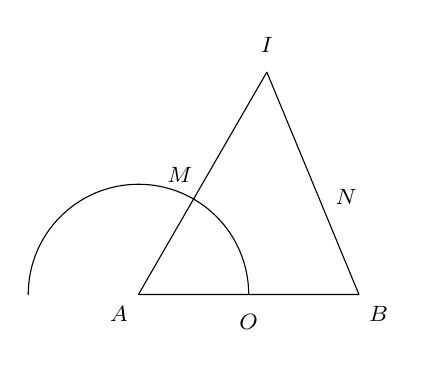
\begin{tikzpicture}[scale=0.7, font=\footnotesize, line join=round, line cap=round, >=stealth]
				\path
				(0,0) coordinate (O)
				(-2,0) coordinate (A)
				(2,0) coordinate (B)
				(120:2) coordinate (M)
				(45:2) coordinate (N)
				(intersection of A--M and B--N) coordinate (I)
				;
				\draw (I)--(A)--(B)--cycle (O)arc(0:180:2cm);
				\foreach \d/\g in {O/-90,A/-135,B/-45,M/120,N/45,I/90}
					{\draw (\d) node [shift=(\g:10pt)]{$\d$};}
			\end{tikzpicture}
		}}
\end{ex}
\begin{ex}%[0H2K2-1]
	Cho hai điểm $M, N$ nằm trên đường tròn đường kính $AB=2r$. Gọi $I$ là giao điểm của hai đường thẳng $AM$ và $BN$. Tính theo $r$ giá trị biểu thức $P=\overrightarrow{AM}\cdot \overrightarrow{AI}+\overrightarrow{BN}\cdot \overrightarrow{BI}$.
	\choice
	{\True $P=4r^2$}
	{$P=2r^2$}
	{$P=r^2$}
	{$P=\dfrac{r^2}{4} $}
	\loigiai{Vì $AI\perp BM$ và $BI\perp AN$ nên $\overrightarrow{AI}\cdot \overrightarrow{BM}=\overrightarrow{BI}\cdot \overrightarrow{AN}=0$.
		\immini{Do đó
			\begin{align*}
				P & =\overrightarrow{AM}\cdot \overrightarrow{AI}+\overrightarrow{BN}\cdot \overrightarrow{BI}                                                                      \\
				  & = \left(\overrightarrow{AB}+\overrightarrow{BM}\right)\cdot \overrightarrow{AI} + \left(\overrightarrow{BA}+\overrightarrow{AN}\right)\cdot \overrightarrow{BI} \\
				  & = \overrightarrow{AB}\cdot \overrightarrow{AI}-\overrightarrow{AB}\cdot \overrightarrow{BI}                                                                     \\
				  & = \overrightarrow{AB}\cdot \left(\overrightarrow{AI}+\overrightarrow{IB}\right)                                                                                 \\
				  & = \overrightarrow{AB}^2=AB^2=4r^2.
			\end{align*}}{
			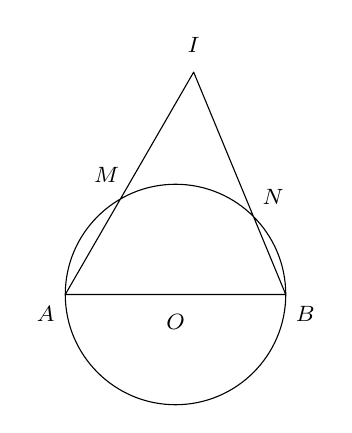
\begin{tikzpicture}[scale=0.7, font=\footnotesize, line join=round, line cap=round, >=stealth]
				\path
				(0,0) coordinate (O)
				(-2,0) coordinate (A)
				(2,0) coordinate (B)
				(120:2) coordinate (M)
				(45:2) coordinate (N)
				(intersection of A--M and B--N) coordinate (I)
				;
				\draw (I)--(A)--(B)--cycle (O)circle(2cm);
				\foreach \d/\g in {O/-90,A/-135,B/-45,M/120,N/45,I/90}
					{\draw (\d) node [shift=(\g:10pt)]{$\d$};}
			\end{tikzpicture}
		}
	}
\end{ex}

% \begin{ex}%[0H2K2-1]
% 	Trong mặt phẳng tọa độ $Oxy$, cho hai véc-tơ $\overrightarrow{a}=(x;x-1),\overrightarrow{b}=(x+2;x+1)$. Điều kiện của $x$ để $\overrightarrow{a}\cdot\overrightarrow{b}<3$ là
% 	\choice
% 	{$-2<x<3$}
% 	{\True $-2<x<1$}
% 	{$0<x<1$}
% 	{$-2<x$}
% 	\loigiai{
% 		Ta có $\overrightarrow{a}\cdot\overrightarrow{b}=x(x+2)+(x-1)(x+1)<3$\\
% 		$\Leftrightarrow x^2+2x+x^2-1-3<0\Leftrightarrow x^2+x-2<0\Leftrightarrow -2<x<1$.
% 	}
% \end{ex}
\begin{ex}%[0H2K2-1]
	Cho hình vuông $ABCD$ có cạnh là $a$. Giá trị của biểu thức $\left(\overrightarrow{BC}+\overrightarrow{BD}+\overrightarrow{BA}\right)\left(\overrightarrow{AC}-\overrightarrow{AB}\right)$ là
	\choice
	{$0$}
	{\True $2a^2$}
	{$-2a^2$}
	{$-2\sqrt{2}a^2$}
	\loigiai{
		$\left(\overrightarrow{BC}+\overrightarrow{BD}+\overrightarrow{BA}\right) \left(\overrightarrow{AC}-\overrightarrow{AB}\right)=2\overrightarrow{BD}\cdot\overrightarrow{BC}=2\big| \overrightarrow{BD}\big| \cdot \big| \overrightarrow{BC}\big| \cdot \cos\left(\overrightarrow{BD},\overrightarrow{BC}\right)=2\cdot  a\sqrt{2}\cdot  a\cdot \dfrac{\sqrt{2}}{2}=2a^2$.
	}
\end{ex}
\begin{ex}%[0H2K2-1]
	Cho hình vuông $ABCD$ cạnh bằng $2$. Điểm $M$ nằm trên đoạn thẳng $AC$ sao cho $AM=\dfrac{AC}{4}$. Gọi $N$ là trung điểm của đoạn thẳng $DC$. Tính $\overrightarrow{MB}\cdot \overrightarrow{MN}$.
	\choice
	{$\overrightarrow{MB}\cdot \overrightarrow{MN}=-4$}
	{\True $\overrightarrow{MB}\cdot \overrightarrow{MN}=0$}
	{$\overrightarrow{MB}\cdot \overrightarrow{MN}=4$}
	{$\overrightarrow{MB}\cdot \overrightarrow{MN}=16$}
	\loigiai{
		Vì giả thiết không cho góc nên ta thử phân tích các véc-tơ $\overrightarrow{MB},\ \overrightarrow{MN}$ theo các véc-tơ có giá vuông góc với nhau.
		\begin{align*}
			\overrightarrow{MB} & =\overrightarrow{AB}-\overrightarrow{AM}=\overrightarrow{AB}-\dfrac{1}{4}\overrightarrow{AC}=\overrightarrow{AB}-\dfrac{1}{4}\left(\overrightarrow{AB}+\overrightarrow{AD}\right)=\dfrac{3}{4}\overrightarrow{AB}-\dfrac{1}{4}\overrightarrow{AD}. \\
			\overrightarrow{MN} & =\overrightarrow{AN}-\overrightarrow{AM}=\overrightarrow{AD}+\overrightarrow{DN}-\dfrac{1}{4}\overrightarrow{AC}=\overrightarrow{AD}+\dfrac{1}{2}\overrightarrow{DC}-\dfrac{1}{4}\left(\overrightarrow{AB}+\overrightarrow{AD}\right)              \\
			                    & =\overrightarrow{AD}+\dfrac{1}{2}\overrightarrow{AB}-\dfrac{1}{4}\left(\overrightarrow{AB}+\overrightarrow{AD}\right)=\dfrac{3}{4}\overrightarrow{AD}+\dfrac{1}{4}\overrightarrow{AB}.
		\end{align*}
		Suy ra
		\begin{align*}
			\overrightarrow{MB}\cdot \overrightarrow{MN} & =\left(\dfrac{3}{4}\overrightarrow{AB}-\dfrac{1}{4}\overrightarrow{AD}\right)\left(\dfrac{3}{4}\overrightarrow{AD}+\dfrac{1}{4}\overrightarrow{AB}\right)=\dfrac{1}{16}\left(3\overrightarrow{AB}\cdot \overrightarrow{AD}+3\overrightarrow{AB}^2-3\overrightarrow{AD}^2-\overrightarrow{AD}\cdot \overrightarrow{AB}\right) \\
			                                             & =\dfrac{1}{16}\left(0+3a^2-3a^2-0\right)=0.
		\end{align*}
	}
\end{ex}
\begin{ex}%[0H2K2-1]
	Cho hình thoi $ABCD$ có $AC=8$. Tính $\overrightarrow{AB}\cdot \overrightarrow{AC}$.
	\choice
	{$\overrightarrow{AB}\cdot \overrightarrow{AC}=24$}
	{$\overrightarrow{AB}\cdot \overrightarrow{AC}=26$}
	{$\overrightarrow{AB}\cdot \overrightarrow{AC}=28$}
	{\True $\overrightarrow{AB}\cdot \overrightarrow{AC}=32$}
	\loigiai{
		Gọi $O=AC\cap BD$, giả thiết không cho góc, ta phân tích các véc-tơ $\overrightarrow{AB},\ \overrightarrow{AC}$ theo các véc-tơ có giá vuông góc với nhau.\\
		Ta có $\overrightarrow{AB}\cdot \overrightarrow{AC}=\left(\overrightarrow{AO}+\overrightarrow{OB}\right)\cdot \overrightarrow{AC}=\overrightarrow{AO}\cdot \overrightarrow{AC}+\overrightarrow{OB}\cdot \overrightarrow{AC}=\dfrac{1}{2}\overrightarrow{AC}\cdot \overrightarrow{AC}+0=\dfrac{1}{2}AC^2=32$.
	}
\end{ex}
\begin{ex}%[0H2K2-1]
	Cho hình chữ nhật $ABCD$ có $AB=a$ và $AD=a\sqrt{2} $. Gọi $K$ là trung điểm của cạnh $AD$. Tính $\overrightarrow{BK}\cdot \overrightarrow{AC}$.
	\choice
	{\True $\overrightarrow{BK}\cdot \overrightarrow{AC}=0$}
	{$\overrightarrow{BK}\cdot \overrightarrow{AC}=-a^2\sqrt{2} $}
	{$\overrightarrow{BK}\cdot \overrightarrow{AC}=a^2\sqrt{2} $}
	{$\overrightarrow{BK}\cdot \overrightarrow{AC}=2a^2$}
	\loigiai{
	Ta có $AC=BD=\sqrt{A{B^2}+A{D^2}}=\sqrt{2a^2+a^2}=a\sqrt{3} $.\\
	Lại có $\left\{
		\begin{array}{l}
			\overrightarrow{BK}=\overrightarrow{BA}+\overrightarrow{AK}=\overrightarrow{BA}+\dfrac{1}{2}\overrightarrow{AD} \\
			\overrightarrow{AC}=\overrightarrow{AB}+\overrightarrow{AD}.
		\end{array}\right.$\\
	$\overrightarrow{BK}\cdot \overrightarrow{AC}=\overrightarrow{BA}\cdot \overrightarrow{AB}+\overrightarrow{BA}\cdot \overrightarrow{AD}+\dfrac{1}{2}\overrightarrow{AD}\cdot \overrightarrow{AB}+\dfrac{1}{2}\overrightarrow{AD}\cdot \overrightarrow{AD}=-a^2+0+0+\dfrac{1}{2}{\left(a\sqrt{2}\right)^2}=0$.
	}
\end{ex}

% \begin{ex}%[0H2K2-1]
% 	Trong hệ trục tọa độ $Oxy$, cho $\overrightarrow{u}=(2;5)$ và $\overrightarrow{v}=(-3;1)$. Tìm số thực $m$ để $\overrightarrow{a}=m\overrightarrow{u}+\overrightarrow{v}$ tạo với $\overrightarrow{b}=(1;1)$ một góc $45^{\circ}$.
% 	\choice
% 	{\True $m=\dfrac{3}{2}$}
% 	{$m=-1$}
% 	{$m=-\dfrac{1}{5}$}
% 	{$m=2$}
% 	\loigiai{
% 		véc-tơ $\overrightarrow{a}=\left( 2m-3; 5m+1\right)$; $\overrightarrow{b}=(1;1)$.
% 		\begin{eqnarray*}
% 			& & \cos\left( \overrightarrow{a},\overrightarrow{b}\right)=\dfrac{\sqrt{2}}{2}\\
% 			& \Leftrightarrow & \dfrac{(2m-3)\cdot 1 + (5m+1)\cdot 1}{\sqrt{(2m-3)^2+(5m+1)^2}\cdot \sqrt{2}}= \dfrac{\sqrt{2}}{2}\\
% 			& \Leftrightarrow & \dfrac{7m-2}{\sqrt{29m^2-2m+10}}=1\\
% 			&\Leftrightarrow & \sqrt{29m^2-2m+10}=7m-2\\
% 			&\Leftrightarrow & \heva{ &7m-2\geq 0 \\ & 29m^2-2m+10=49m^2-28m+4}\\
% 			&\Leftrightarrow & \heva{
% 				& m \geq \dfrac{2}{7} \\ & 20m^2-26m-6=0
% 			} \Leftrightarrow m=\dfrac{3}{2}.
% 		\end{eqnarray*}
% 	}
% \end{ex}

\begin{ex}%[0H2K2-1]
	Cho tứ giác $ABCD$ có hai đường chéo vuông góc với nhau tại $M$ và $\overrightarrow {MA}\cdot \overrightarrow {MC}=\overrightarrow {MB}\cdot \overrightarrow {MD}$. Gọi $P$ là trung điểm của $AD$. Góc giữa hai đường thẳng $MP$ và $BC$ là
	\choice
	{\True $90^\circ $}
	{$60^\circ $}
	{$45^\circ $}
	{$30^\circ $}
	\loigiai {Ta có $\overrightarrow {BC}=\overrightarrow {MC}-\overrightarrow {MB};\overrightarrow {MP}=\dfrac {1}{2} \left(\overrightarrow {MA}+\overrightarrow {MD}\right)$\\
		Suy ra $2\overrightarrow {MP}\cdot \overrightarrow {BC}=\left(\overrightarrow {MC}-\overrightarrow {MB}\right)\left(\overrightarrow {MA}+\overrightarrow {MD}\right)$ \\
		$=\overrightarrow {MA}\cdot \overrightarrow {MC}+\overrightarrow {MC}\cdot \overrightarrow {MD}-\overrightarrow {MA}\cdot \overrightarrow {MB}-\overrightarrow {MB}\cdot \overrightarrow {MD}$\\
		$=\overrightarrow {MC}\cdot \overrightarrow {MD}-\overrightarrow {MA}\cdot \overrightarrow {MB}=0$ (Vì $\overrightarrow {MA}\cdot \overrightarrow {MC}=\overrightarrow {MB}\cdot \overrightarrow {MD}$ và $\overrightarrow {MA}\cdot \overrightarrow {MB}=\overrightarrow {MC}\cdot \overrightarrow {MD}=0$)\\
		Vậy $MP\perp BC\Rightarrow \widehat {\left(MP,BC\right)}=90^\circ $.}
\end{ex}

\begin{ex}%[0H2K2-1]
	Cho hình vuông $ABCD$ cạnh $a$. Gọi $M$ và $N$ lần lượt là trung điểm của $BC$ và $CD$. Tính $\cos \left(\overrightarrow {AM},\overrightarrow {NA}\right)$.
	\choice
	{$\dfrac {4}{5}$}
	{\True $-\dfrac {4}{5}$}
	{$\dfrac {3}{5}$}
	{$-\dfrac {3}{5}$}
	\loigiai {
	\immini {
	Từ giả thiết ta có $AM=AN=\dfrac {a\sqrt{5}}{2} $.\\
	$\overrightarrow {AM}=\overrightarrow {AB}+\overrightarrow {BM};\overrightarrow {NA}=\overrightarrow {ND}+\overrightarrow {DA}$ \\
	$\Rightarrow \overrightarrow {AM}\cdot \overrightarrow {NA}=\left(\overrightarrow {AB}+\overrightarrow {BM}\right)\left(\overrightarrow {ND}+\overrightarrow {DA}\right)$\\
	$=\overrightarrow {AB}\cdot \overrightarrow {ND}+\overrightarrow {AB}\cdot \overrightarrow {DA}+\overrightarrow {BM}\cdot \overrightarrow {ND}+\overrightarrow {BM}\cdot \overrightarrow {DA}$\\
	$=a\cdot \dfrac {a}{2} \cdot \cos 180^\circ +0+0+a\cdot \dfrac {a}{2} \cdot \cos 180^\circ =-a^{2} $ \\
	Suy ra $\cos \left(\overrightarrow {AM},\overrightarrow {NA}\right)=\dfrac {\overrightarrow {AM}\cdot \overrightarrow {NA}}{\big| \overrightarrow {AM}\big| \cdot \big| \overrightarrow {NA}\big| } =\dfrac {-a^{2}}{\dfrac {a\sqrt{5}}{2} \cdot \dfrac {a\sqrt{5}}{2}} =-\dfrac {4}{5}$.}
	{
	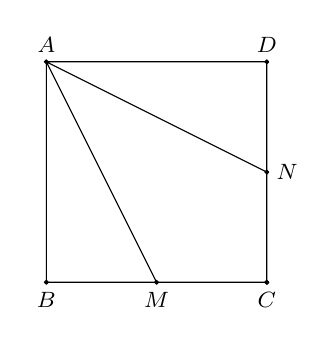
\begin{tikzpicture}[scale=0.7, font=\footnotesize, line join=round, line cap=round, >=stealth]
		\draw(0,0) node[below]{$B$}--(2,0) node[below]{$M$}--(4,0) circle (1pt) node[below]{$C$}--(4,2) node[right]{$N$}--(4,4) node[above]{$D$}--(0,4) node[above]{$A$}--(0,0) (0,4)--(4,2) (0,4)--(2,0);
		\draw [fill=black] (0,0) circle (1pt);
		\draw [fill=black] (2,0) circle (1pt);
		\draw [fill=black] (4,0) circle (1pt);
		\draw [fill=black] (4,2) circle (1pt);
		\draw [fill=black] (4,4) circle (1pt);
		\draw [fill=black] (0,4) circle (1pt);
	\end{tikzpicture}
	}
	}
\end{ex}
\begin{ex}%[0H2G1-4]
	Cho hình vuông $ABCD$. Gọi $M$ là trung điểm của cạnh $BC$. Tính góc giữa hai véc-tơ $\overrightarrow{AM}$ và $\overrightarrow{DA}+\overrightarrow{DB}$.
	\choice
	{$45^\circ$}
	{$30^\circ$}
	{$135^\circ$}
	{\True $90^\circ$}
	\loigiai{
		\immini{Gọi $N$ là trung điểm $AB$.\\
			Có $\overrightarrow{DA}+\overrightarrow{DB}=2\overrightarrow{DN}$\\
			Chứng minh được $AM\perp DN$\\
			Suy ra góc giữa hai véc-tơ $\overrightarrow{AM}$ và $\overrightarrow{DA}+\overrightarrow{DB}$ bằng $\left(\overrightarrow{AM},\overrightarrow{DN}\right)=90^\circ$.}
		{
			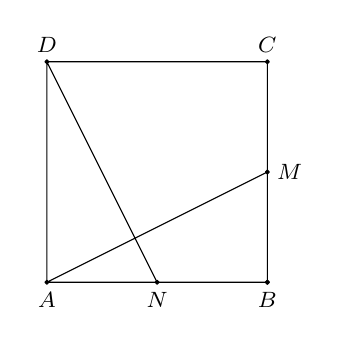
\begin{tikzpicture}[scale=0.7, font=\footnotesize, line join=round, line cap=round, >=stealth]
				\draw(0,0) node[below]{$A$}--(2,0) node[below]{$N$}--(4,0) circle (1pt) node[below]{$B$}--(4,2) node[right]{$M$}--(4,4) node[above]{$C$}--(0,4) node[above]{$D$}--(0,0)--(4,2) (0,4)--(2,0);
				\draw [fill=black] (0,0) circle (1pt);
				\draw [fill=black] (2,0) circle (1pt);
				\draw [fill=black] (4,0) circle (1pt);
				\draw [fill=black] (4,2) circle (1pt);
				\draw [fill=black] (4,4) circle (1pt);
				\draw [fill=black] (0,4) circle (1pt);
			\end{tikzpicture}}
	}
\end{ex}
\begin{ex}%[0H2G1-4]
	Cho hình vuông $ABCD$. Trên cạnh $AD, AB$ lần lượt lấy hai điểm $E, F$ sao cho
	$AE=AF$. Gọi $H$ là hình chiếu vuông góc của $A$ lên đường thẳng $BE$. Tính $\cos \left(\overrightarrow{FH},\overrightarrow{CH}\right)$.
	\choice{\True$0$}
	{$\displaystyle \frac{\sqrt{3}}{2}$}
	{$\displaystyle \frac{-1}{2}$}
	{$\displaystyle \frac{\sqrt{2}}{2}$}
	\loigiai{
		\immini{Gọi $K=AH\cap CD$. Khi đó $BCKF$ là hình chữ nhật.\\
			Ta có $\widehat{BHK}=90^\circ$. \\
			Do đó $H$ thuộc đường tròn ngoại tiếp hình chữ nhật $BCKF$.\\
			$\Rightarrow \widehat{CHF}=90^\circ \Rightarrow \left(\overrightarrow{FH},\overrightarrow{CH}\right)=90^\circ \Rightarrow \cos \left(\overrightarrow{FH},\overrightarrow{CH}\right)=0$.}{
			\begin{tikzpicture}[scale=0.7, font=\footnotesize, line join=round, line cap=round, >=stealth]
				\tkzInit[xmin=-1,xmax=5,ymin=-1,ymax=5]
				\tkzClip
				\tkzDefPoints{ 0/0/D, 0/4/A, 4/4/B, 4/0/C, 3/4/F, 3/0/K, 0/1/E, 1.425/2.1/H}
				\tkzDrawSegments(A,B B,C C,D D,A A,K H,F F,K F,C K,B E,B H,C)
				\tkzMarkRightAngles(A,H,E K,H,B)
				\tkzDrawPoints(A,B,C,D,E,F,K,H)
				\tkzLabelPoints[above](A,B,F)
				\tkzLabelPoints[below](D,K,C,H)
				\tkzLabelPoints[left](E)
			\end{tikzpicture}}
	}
\end{ex}
%%%%%%%%%%%%%%%%%%%%%%%%%%%%%%%%%%%%%%%





% %%%Phần thầy Lê Minh An
% \begin{ex}%[0H2B2-2]
% 	Để $\overrightarrow{u}\cdot\overrightarrow{v}=\left|\overrightarrow{u}\right|\cdot\left|\overrightarrow{v}\right|$ thì $\overrightarrow{u}$ và $\overrightarrow{v}$ phải là hai véc-tơ
% 	\choice
% 	{cùng phương}
% 	{\True cùng hướng}
% 	{ngược hướng}
% 	{vuông góc}
% 	\loigiai
% 	{
% 		Để thỏa mãn đề bài thì $\cos\left(\overrightarrow{u},\overrightarrow{v}\right)=1\Leftrightarrow\left(\overrightarrow{u},\overrightarrow{v}\right)=0$.\\
% 		Vậy $\overrightarrow{u}$ và $\overrightarrow{v}$ phải là hai véc-tơ cùng hướng.
% 	}
% \end{ex}

% \begin{ex}%[0H2B2-2]
% 	Để $\overrightarrow{u}\cdot\overrightarrow{v}=-\left|\overrightarrow{u}\right|\cdot\left|\overrightarrow{v}\right|$ thì $\overrightarrow{u}$ và $\overrightarrow{v}$ phải là hai véc-tơ
% 	\choice
% 	{cùng phương}
% 	{cùng hướng}
% 	{\True ngược hướng}
% 	{vuông góc}
% 	\loigiai
% 	{
% 		Để thỏa mãn đề bài thì $\cos\left(\overrightarrow{u},\overrightarrow{v}\right)=-1\Leftrightarrow\left(\overrightarrow{u},\overrightarrow{v}\right)=180$.\\
% 		Vậy $\overrightarrow{u}$ và $\overrightarrow{v}$ phải là hai véc-tơ ngược hướng.
% 	}
% \end{ex}

% \begin{ex}%[0H2B2-2]
% 	Cho $M$ là trung điểm $AB$, đẳng thức nào {\bf{sai}} ?
% 	\choice
% 	{$\overrightarrow{MA}\cdot \overrightarrow{AB}=-MA\cdot AB$}
% 	{\True $\overrightarrow{MA}\cdot \overrightarrow{MB}=MA \cdot MB$}
% 	{$\overrightarrow{AM}\cdot \overrightarrow{AB}=AM \cdot AB$}
% 	{$\overrightarrow{MA} \cdot \overrightarrow{MB}=-MA \cdot MB$}
% 	\loigiai
% 	{ \begin{itemize}
% 			\item Do $M$ là trung điểm của $AB$ nên $\left( \overrightarrow{MA}, \overrightarrow{MB}\right) =180 ^\circ$.\\
% 			Ta có $\overrightarrow{MA}\cdot \overrightarrow{MB}=MA \cdot MB \cdot \cos \left(\overrightarrow{MA}, \overrightarrow{MB} \right) = MA \cdot MB \cdot \cos 180^\circ =-MA\cdot MB.$
% 			\item Do $M$ là trung điểm của $AB$ nên $\left( \overrightarrow{MA}, \overrightarrow{AB}\right) =180 ^\circ$.\\
% 			Ta có $\overrightarrow{MA}\cdot \overrightarrow{AB}=MA \cdot AB \cdot \cos \left(\overrightarrow{MA}, \overrightarrow{AB} \right) = MA \cdot AB \cdot \cos 180^\circ =-MA\cdot AB.$
% 			\item Do $M$ là trung điểm của $AB$ nên $\left( \overrightarrow{AM}, \overrightarrow{AB}\right) =0 ^\circ$.\\
% 			Ta có $\overrightarrow{AM}\cdot \overrightarrow{AB}=MA \cdot AB \cdot \cos \left(\overrightarrow{AM}, \overrightarrow{AB} \right) = MA \cdot AB \cdot \cos 0^\circ =AM\cdot AB.$
% 		\end{itemize}
% 	}
% \end{ex}

% \begin{ex}%[0H2B2-2]
% 	Cho hình vuông $ABCD$ tâm $O$ khẳng định nào sau đây là \textbf{sai}?
% 	\choice
% 	{\True $\overrightarrow{AB}\cdot\overrightarrow{CD}=\overrightarrow{AD}\cdot\overrightarrow{BC}$}
% 	{$\overrightarrow{AO}\cdot\overrightarrow{OC}=\overrightarrow{BO}\cdot\overrightarrow{OD}$}
% 	{$\overrightarrow{AO}\cdot\overrightarrow{OB}=\overrightarrow{DO}\cdot\overrightarrow{OC}$}
% 	{$\overrightarrow{AC}\cdot\overrightarrow{BD}=\overrightarrow{AD}\cdot\overrightarrow{AB}$}
% 	\loigiai
% 	{
% 		\immini
% 		{
% 			Giả sử hình vuông có cạnh bằng $1$.
% 			\begin{itemize}
% 				\item $\overrightarrow{AB}\cdot\overrightarrow{CD}=AB\cdot CD\cdot\cos 180^\circ=-1$, $\overrightarrow{AD}\cdot\overrightarrow{BC}=AD\cdot BC\cdot\cos 0^\circ=1$.
% 				\item $\overrightarrow{AO}\cdot\overrightarrow{OC}=AO\cdot OC\cdot\cos 0^\circ=\dfrac{1}{2}$, $\overrightarrow{BO}\cdot\overrightarrow{OD}=BO\cdot OD\cdot\cos 0^\circ=\dfrac{1}{2}$.
% 				\item $\overrightarrow{AO}\cdot\overrightarrow{OB}=\overrightarrow{DO}\cdot\overrightarrow{OC}=0$.
% 				\item $\overrightarrow{AC}\cdot\overrightarrow{BD}=\overrightarrow{AD}\cdot\overrightarrow{AB}=0$.
% 			\end{itemize}
% 		}
% 		{
% 			\begin{tikzpicture}[scale=.7,font=\footnotesize, line join=round, line cap=round, >=stealth]
% 				\tkzDefPoints{0/0/A,3/0/B,3/-3/C,0/-3/D}
% 				\tkzInterLL(A,C)(B,D)    \tkzGetPoint{O}
% 				\draw (A)--(B)--(C)--(D)--(A)--(C)
% 				(B)--(D);
% 				\foreach \x/\g in {A/150,B/60,C/-60,D/-150,O/90} \fill[black](\x) circle (1pt) ($(\x)+(\g:3mm)$) node{\x};
% 			\end{tikzpicture}
% 		}
% 	}
% \end{ex}

% \begin{ex}%[0H2B2-2]
% 	Cho hình thoi $ABCD$, khẳng định nào sau đây là đúng?
% 	\choice
% 	{$\overrightarrow{AB}\cdot\overrightarrow{AD}=\overrightarrow{DA}\cdot\overrightarrow{DC}$}
% 	{$\overrightarrow{AB}\cdot\overrightarrow{AC}=\overrightarrow{AC}\cdot\overrightarrow{CD}$}
% 	{$\overrightarrow{AC}\cdot\overrightarrow{BD}=\overrightarrow{AB}\cdot\overrightarrow{AD}$}
% 	{\True $\overrightarrow{BA}\cdot\overrightarrow{BC}=\overrightarrow{DA}\cdot\overrightarrow{DC}$}
% 	\loigiai
% 	{
% 		\immini
% 		{
% 			Giả sử hình thoi có cạnh bằng $1$.
% 			\begin{itemize}
% 				\item $\overrightarrow{AB}\cdot\overrightarrow{AD}=\cos\widehat{BAD}$, $\overrightarrow{DA}\cdot\overrightarrow{DC}=\cos\widehat{ADC}$ nhưng $\cos\widehat{BAD}\neq \cos\widehat{ADC}$.\\
% 				Nên $\overrightarrow{AB}\cdot\overrightarrow{AD}\neq \overrightarrow{DA}\cdot\overrightarrow{DC}$.
% 				\item $\overrightarrow{AB}\cdot\overrightarrow{AC}=AC\cdot\cos\widehat{BAC}$, $\overrightarrow{AC}\cdot\overrightarrow{CD}=-AC\cdot\cos\widehat{ACD}$, mà $\widehat{BAC}=\widehat{ACD}$.\\
% 				Nên $\overrightarrow{AB}\cdot\overrightarrow{AC}\neq \overrightarrow{AC}\cdot\overrightarrow{CD}$.
% 				\item $\overrightarrow{AC}\cdot\overrightarrow{BD}=0$ nhưng $\overrightarrow{AB}\cdot\overrightarrow{AD}\neq 0$, nên $\overrightarrow{AC}\cdot\overrightarrow{BD}\neq \overrightarrow{AB}\cdot\overrightarrow{AD}$.
% 				\item $\overrightarrow{BA}\cdot\overrightarrow{BC}=\cos\widehat{ABC}$, $\overrightarrow{DA}\cdot\overrightarrow{DC}=\cos\widehat{ADC}$. Mà $\widehat{ABC}=\widehat{ADC}$. Nên $\overrightarrow{BA}\cdot\overrightarrow{BC}=\overrightarrow{DA}\cdot\overrightarrow{DC}$.
% 			\end{itemize}
% 		}
% 		{
% 			\begin{tikzpicture}[scale=.8,font=\footnotesize, line join=round, line cap=round, >=stealth]
% 				\tkzDefPoints{0/0/B,3/0/D,1.5/1/A,1.5/-1/C}
% 				\draw (A)--(B)--(C)--(D)--(A)--(C)
% 				(B)--(D);
% 				\foreach \x/\g in {A/90,B/180,D/0,C/-90} \fill[black](\x) circle (1pt) ($(\x)+(\g:3mm)$) node{\x};
% 			\end{tikzpicture}
% 		}
% 	}
% \end{ex}

% \begin{ex}%[0H2B2-2]
% 	Cho hình bình hành $ABCD$ và điểm $E$ tùy ý, khi đó $\overrightarrow{AB}\cdot\overrightarrow{EA}+\overrightarrow{AD}\cdot\overrightarrow{EA}+\overrightarrow{CE}\cdot\overrightarrow{EA}$ bằng
% 	\choice
% 	{$AE^2$}
% 	{\True $-AE^2$}
% 	{$AE\cdot CE$}
% 	{$-AE\cdot DE$}
% 	\loigiai
% 	{
% 		Ta có $\overrightarrow{AB}+\overrightarrow{AD}+\overrightarrow{CE}=\overrightarrow{AC}+\overrightarrow{CE}=\overrightarrow{AE}$.\\
% 		Suy ra $\overrightarrow{AB}\cdot\overrightarrow{EA}+\overrightarrow{AD}\cdot\overrightarrow{EA}+\overrightarrow{CE}\cdot\overrightarrow{EA}=\overrightarrow{AE}\cdot\overrightarrow{EA}=-AE^2$.
% 	}
% \end{ex}

\begin{ex}%[0H2K2-2]
	Cho hai điểm $A$ và $B$, $O$ là trung điểm của $AB$ và $M$ là điểm tùy ý, biết rằng $\overrightarrow{MA}\cdot\overrightarrow{MB}=OM^2+kOA^2$. Khẳng định nào sau đây đúng?
	\choice
	{$k=1$}
	{\True $k=-1$}
	{$k=2$}
	{$k=-2$}
	\loigiai
	{
		Ta có $O$ là trung điểm $AB$ nên $\overrightarrow{OA}+\overrightarrow{OB}=\overrightarrow{0}$. Do đó
		\begin{eqnarray*}
			\overrightarrow{MA}\cdot\overrightarrow{MB}
			& = & \left(\overrightarrow{MO}+\overrightarrow{OA}\right)\cdot\left(\overrightarrow{MO}+\overrightarrow{OB}\right)\\
			& = & \overrightarrow{MO}^2+\overrightarrow{MO}\left(\overrightarrow{OA}+\overrightarrow{OB}\right)+\overrightarrow{OA}\cdot\overrightarrow{OB}\\
			& = & OM^2-OA^2.
		\end{eqnarray*}
		Vậy $k=-1$.
	}
\end{ex}

\begin{ex}%[0H2K2-2]
	Cho $I$ là trung điểm $AB$, $M$ là điểm tùy ý. Biết rằng $\overrightarrow{MI}\cdot\overrightarrow{AB}=k\left(MB^2-MA^2\right)$. Khẳng định nào sau đây là đúng?
	\choice
	{$k=2$}
	{\True $k=\dfrac{1}{2}$}
	{$k=-1$}
	{$k=-\dfrac{1}{2}$}
	\loigiai
	{
		Ta có $I$ là trung điểm $AB$ nên $\overrightarrow{MA}+\overrightarrow{MB}=2\overrightarrow{MI}$. Do đó
		\begin{eqnarray*}
			MB^2-MA^2
			& = & \overrightarrow{MB}^2-\overrightarrow{MA}^2\\
			& = & \left(\overrightarrow{MB}-\overrightarrow{MA}\right)\cdot\left(\overrightarrow{MB}+\overrightarrow{MA}\right)\\
			& = & \overrightarrow{AB}\cdot\left(2\overrightarrow{MI}\right)\\
			& = & 2\overrightarrow{MI}\cdot\overrightarrow{AB}.
		\end{eqnarray*}
		$\Rightarrow \overrightarrow{MI}\cdot\overrightarrow{AB}=\dfrac{1}{2}\left(MB^2-MA^2\right)$. Vậy $k=\dfrac{1}{2}$.
	}
\end{ex}

\begin{ex}%[0H2K2-2]
	Cho $I$ là trung điểm $AB$, $M$ là điểm tùy ý. Biết rằng $\overrightarrow{MA}\cdot\overrightarrow{MB}=MI^2+kAB^2$. Khẳng định nào sau đây là đúng?
	\choice
	{$k=2$}
	{$k=\dfrac{1}{2}$}
	{$k=-1$}
	{\True $k=-\dfrac{1}{4}$}
	\loigiai
	{
		Ta có $I$ là trung điểm $AB$ nên $\overrightarrow{IA}+\overrightarrow{IB}=0$. Do đó
		\begin{eqnarray*}
			\overrightarrow{MA}\cdot\overrightarrow{MB}
			& = & \left(\overrightarrow{MI}+\overrightarrow{IA}\right)\left(\overrightarrow{MI}+\overrightarrow{IB}\right)\\
			& = & \overrightarrow{MI}^2+\overrightarrow{MI}\left(\overrightarrow{IA}+\overrightarrow{IB}\right)+\overrightarrow{IA}\cdot\overrightarrow{IB}\\
			MI^2-\dfrac{1}{4}AB^2.
		\end{eqnarray*}
		Vậy $k-\dfrac{1}{4}$.
	}
\end{ex}


\begin{ex}%[0H2K2-2]
	Khẳng định nào sau đây là đúng?
	\choice
	{$\left(\overrightarrow{a}\cdot\overrightarrow{b}\right)\overrightarrow{c}=\overrightarrow{a}\left(\overrightarrow{b}\cdot\overrightarrow{c}\right)$}
	{$\left(\overrightarrow{a}\cdot\overrightarrow{b}\right)^2=\overrightarrow{a}^2\cdot\overrightarrow{b}^2$}
	{$\overrightarrow{a}\cdot\overrightarrow{b}=\left|\overrightarrow{a}\right|\cdot\left|\overrightarrow{b}\right|\sin\left(\overrightarrow{a},\overrightarrow{b}\right)$}
	{\True $\overrightarrow{a}\cdot\left(\overrightarrow{b}-\overrightarrow{c}\right)=\overrightarrow{a}\cdot\overrightarrow{b}-\overrightarrow{a}\cdot\overrightarrow{c}$}
	\loigiai{
		\begin{itemize}
			\item Xét hình vuông $ABCD$ cạnh bằng $1$ thì
			      \begin{itemize}
				      \item $\left(\overrightarrow{AB}\cdot\overrightarrow{AD}\right)\overrightarrow{BC}=0\cdot\overrightarrow{BC}=\overrightarrow{0}$.
				      \item $\overrightarrow{AB}\left(\overrightarrow{AD}\cdot\overrightarrow{BC}\right)=\overrightarrow{AB}\cdot 1=\overrightarrow{AB}\neq \overrightarrow{0}$.
			      \end{itemize}
			      Do đó $\left(\overrightarrow{a}\cdot\overrightarrow{b}\right)\overrightarrow{c}=\overrightarrow{a}\left(\overrightarrow{b}\cdot\overrightarrow{c}\right)$ là khẳng định sai.
			\item Xét hình vuông $ABCD$ cạnh bằng $1$ thì
			      \begin{itemize}
				      \item $\left(\overrightarrow{AB}\cdot\overrightarrow{AD}\right)^2=0^2=0$.
				      \item $\overrightarrow{AB}^2\cdot \overrightarrow{AD}^2=1\cdot 1=1$.
			      \end{itemize}
			      Do đó $\left(\overrightarrow{a}\cdot\overrightarrow{b}\right)^2=\overrightarrow{a}^2\cdot\overrightarrow{b}^2$ là khẳng định sai.
			\item Ta có $\overrightarrow{a}\cdot\overrightarrow{b}=\left|\overrightarrow{a}\right|\cdot\left|\overrightarrow{b}\right|\cos\left(\overrightarrow{a},\overrightarrow{b}\right)$ nên $\overrightarrow{a}\cdot\overrightarrow{b}=\left|\overrightarrow{a}\right|\cdot\left|\overrightarrow{b}\right|\sin\left(\overrightarrow{a},\overrightarrow{b}\right)$ là khẳng định sai.
			\item Ta có $\overrightarrow{a}\cdot\left(\overrightarrow{b}-\overrightarrow{c}\right)=\overrightarrow{a}\cdot\left(\overrightarrow{b}+\left(-\overrightarrow{c}\right)\right)=\overrightarrow{a}\cdot\overrightarrow{b}+\overrightarrow{a}\cdot\left(-\overrightarrow{c}\right)=\overrightarrow{a}\cdot\overrightarrow{b}-\overrightarrow{a}\cdot\overrightarrow{c}$.
		\end{itemize}
	}
\end{ex}

\begin{ex}%[0H2K2-2]
	Cho hai véc-tơ $\overrightarrow{a}$ và $\overrightarrow{b}$. Đẳng thức nào sau đây \textbf{sai}?
	\choice
	{$\overrightarrow{a}\cdot\overrightarrow{b}=\dfrac{1}{4}\left(\left|\overrightarrow{a}+\overrightarrow{b}\right|^2-\left|\overrightarrow{a}-\overrightarrow{b}\right|^2\right)$}
	{\True $\overrightarrow{a}\cdot\overrightarrow{b}=\dfrac{1}{2}\left(\left|\overrightarrow{a}+\overrightarrow{b}\right|^2-\left|\overrightarrow{a}-\overrightarrow{b}\right|^2\right)$}
	{$\overrightarrow{a}\cdot\overrightarrow{b}=\dfrac{1}{2}\left(\left|\overrightarrow{a}+\overrightarrow{b}\right|^2-\left|\overrightarrow{a}\right|^2-\left|\overrightarrow{b}\right|^2\right)$}
	{$\overrightarrow{a}\cdot\overrightarrow{b}=\dfrac{1}{2}\left(\left|\overrightarrow{a}\right|^2+\left|\overrightarrow{b}\right|^2-\left|\overrightarrow{a}-\overrightarrow{b}\right|^2\right)$}
	\loigiai{
		Ta có
		\begin{itemize}
			\item $\left|\overrightarrow{a}+\overrightarrow{b}\right|^2=\left(\overrightarrow{a}+\overrightarrow{b}\right)^2=\overrightarrow{a}^2+2\overrightarrow{a}\cdot\overrightarrow{b}+\overrightarrow{b}^2$.
			\item $\left|\overrightarrow{a}-\overrightarrow{b}\right|^2=\left(\overrightarrow{a}-\overrightarrow{b}\right)^2=\overrightarrow{a}^2-2\overrightarrow{a}\cdot\overrightarrow{b}+\overrightarrow{b}^2$.
		\end{itemize}
		Suy ra
		$$\left|\overrightarrow{a}+\overrightarrow{b}\right|^2-\left|\overrightarrow{a}-\overrightarrow{b}\right|^2=4\overrightarrow{a}\cdot\overrightarrow{b}\Rightarrow \overrightarrow{a}\cdot\overrightarrow{b}=\dfrac{1}{4}\left(\left|\overrightarrow{a}+\overrightarrow{b}\right|^2-\left|\overrightarrow{a}-\overrightarrow{b}\right|^2\right).$$
	}
\end{ex}

\begin{ex}%[0H2K2-2]
	Cho hình thoi $ABCD$ có cạnh bằng $a$ và $\widehat{A}=60^\circ$, điểm $M$ tùy ý. Biết rằng
	$MA^2-MB^2+MC^2-MD^2=ka^2$. Khẳng định nào sau đây đúng?
	\choice
	{\True $k=1$}
	{$k=2$}
	{$k=4$}
	{$k=6$}
	\loigiai
	{
		Ta có $ABCD$ là hình thoi cạnh $a$ và $\widehat{A}=60^\circ$ nên $\triangle ABC$ đều cạnh $a$ do đó $OB=OD=\dfrac{a}{2}$, $OA=OC=\dfrac{a\sqrt{3}}{2}$. Do đó
		\begin{eqnarray*}
			&& MA^2-MB^2+MC^2-MD^2\\
			& = & \left(\overrightarrow{MO}+\overrightarrow{OA}\right)^2-\left(\overrightarrow{MO}+\overrightarrow{OA}\right)^2+\left(\overrightarrow{MO}+\overrightarrow{OC}\right)^2-\left(\overrightarrow{MO}+\overrightarrow{OD}\right)^2\\
			& = & 2\overrightarrow{MO}\left(\overrightarrow{OA}-\overrightarrow{OB}+\overrightarrow{OC}-\overrightarrow{OD}\right)+OA^2-OB^2+OC^2-OD^2\\
			& = & 2\overrightarrow{MO}\left(\overrightarrow{BA}+\overrightarrow{DC}\right)+\dfrac{3a^2}{4}-\dfrac{a^2}{4}+\dfrac{3a^2}{4}-\dfrac{a^2}{4}\\
			& = & a^2.
		\end{eqnarray*}
		Vậy $k=1$.
	}
\end{ex}

\begin{ex}%[0H2K2-2]
	Cho hình chữ nhật $ABCD$ có $O$ là giao điểm của hai đường chéo $AC$ và $BD$, $M$ là điểm tuỳ ý. Biết rằng $\overrightarrow{MA}\cdot \overrightarrow{MC}=MO^2+kBD^2$. Khẳng định nào sau đây đúng?
	\choice
	{$k=-\dfrac{1}{2}$}
	{$k=2$}
	{\True $k=-\dfrac{1}{4}$}
	{$k=4$}
	\loigiai{
	Do $O$ là trung điểm của $AC$ nên $\overrightarrow{MA}+\overrightarrow{MC}=2\overrightarrow{MO} \Rightarrow {\left(\overrightarrow{MA}+\overrightarrow{MC}\right)}^2={\left(2\overrightarrow{MO}\right)}^2$ \\
	$ \Rightarrow MA^2+MC^2+2\overrightarrow{MA}\cdot \overrightarrow{MC}=4MO^2$. \qquad$(1)$ \\
	Lại có $\overrightarrow{MC}-\overrightarrow{MA}=\overrightarrow{AC} \Rightarrow {\left(\overrightarrow{MC}-\overrightarrow{MA}\right)}^2={\left(\overrightarrow{AC}\right)}^2$\\
	$\Rightarrow MA^2+MC^2-2\overrightarrow{MA}\cdot \overrightarrow{MC}=AC^2$.\qquad $(2)$ \\
	Từ (1) và (2), trừ vế theo vế ta được: \\
	$4\overrightarrow{MA}\cdot \overrightarrow{MC}=4MO^2-AC^2 \Rightarrow \overrightarrow{MA}\cdot \overrightarrow{MC}=MO^2-\dfrac{1}{4}BD^2$ (do $AC^2=BD^2$ ).\\
	Vậy $k=-\dfrac{1}{4}$.
	}
\end{ex}

\begin{ex}%[0H2K2-2]
	Cho tam giác $ABC$, gọi $H$ là trực tâm của tam giác và $M$ là trung điểm của cạnh $BC$. Đẳng thức nào sau đây \textbf{đúng}?
	\choice
	{$\overrightarrow{MH} \cdot \overrightarrow{MA}=\dfrac{1}{2}BC^2$}
	{$\overrightarrow{MH} \cdot\overrightarrow{MA}=-\dfrac{1}{4}BC^2$}
	{\True $\overrightarrow{MH} \cdot\overrightarrow{MA}=\dfrac{1}{4}BC^2$}
	{$\overrightarrow{MH} \cdot\overrightarrow{MA}=\dfrac{1}{5}BC^2$}
	\loigiai{
		\immini{
			M là trung điểm của BC, ta có $\heva{& \overrightarrow{MH}= \dfrac{1}{2} (\overrightarrow{BH} +\overrightarrow{CH})\\&\overrightarrow{MA}= \dfrac{1}{2} (\overrightarrow{BA}+\overrightarrow{CA})} $\\
			$\Rightarrow \overrightarrow{MH} \cdot \overrightarrow{MA}
				= \dfrac{1}{4}(\overrightarrow{BA} \cdot \overrightarrow{BH} +\overrightarrow{CA} \cdot \overrightarrow{BH} +\overrightarrow{BA} \cdot \overrightarrow{CH} +\overrightarrow{CA} \cdot \overrightarrow{CH})$\\
			Do $H$ là trực tâm nên lại có
			$$\overrightarrow{BA} \cdot \overrightarrow{BH} = \overrightarrow{BA} \cdot \overrightarrow{BC},\ \overrightarrow{CA} \cdot \overrightarrow{CH} = \overrightarrow{CA} \cdot \overrightarrow{CB},$$
			suy ra
		}{
			\begin{tikzpicture}[scale=.7,font=\footnotesize, line join=round, line cap=round, >=stealth]
				\tkzDefPoints{0/0/B,5/0/C}
				\coordinate (D) at ($(B)!.35!(C)$);
				\coordinate (M) at ($(C)!0.5!(B)$);
				\coordinate (A) at ($(D)+(0,4)$);
				\tkzDefPointBy[projection = onto A--C](B)\tkzGetPoint{E}
				\tkzInterLL(A,D)(B,E)\tkzGetPoint{H}
				\draw (A)--(B)--(C)--(A)--(D)
				(A)--(M)--(H) (B)--(H)--(C);
				\foreach \x/\g in {A/90,B/190,C/-10,H/180,M/-90} \fill[black](\x) circle (1pt) ($(\x)+(\g:3mm)$) node{\x};
			\end{tikzpicture}
		}
		\begin{eqnarray*}
			\overrightarrow{MH} \cdot \overrightarrow{MA}
			&=&\dfrac{1}{4}(\overrightarrow{BA} \cdot \overrightarrow{BC} +\overrightarrow{BA} \cdot \overrightarrow{CH} +\overrightarrow{CB} \cdot \overrightarrow{CA} +\overrightarrow{BH} \cdot \overrightarrow{CA})\\
			&=&\dfrac{1}{4}(\overrightarrow{BA} \cdot \overrightarrow{BH} + \overrightarrow{CA} \cdot \overrightarrow{CH}) \\
			&=&\dfrac{1}{4}(\overrightarrow{BA} \cdot \overrightarrow{BC} - \overrightarrow{CA} \cdot \overrightarrow{BC})\\
			&=&\dfrac{1}{4}\overrightarrow{BC}(\overrightarrow{BA} -\overrightarrow{CA})\\
			&=& \dfrac{1}{4}BC^2.
		\end{eqnarray*}
	}
\end{ex}

\begin{ex}%[0H2K2-2]
	Cho điểm $M$ thay đổi trên đường tròn tâm $O$ bán kính $R$ ngoại tiếp tam giác đều $ABC$ cho trước. Biết rằng $MA^2+2\overrightarrow{MB}\cdot\overrightarrow{MC}=kR^2$. Khẳng định nào sau đây đúng?
	\choice
	{$k=2$}
	{\True $k=3$}
	{$k=4$}
	{$k=6$}
	\loigiai{
		Ta có $\triangle ABC$ đều nên $\widehat{BOC}=2\widehat{BAC}=120^\circ$, $\overrightarrow{OA}+\overrightarrow{OB}+\overrightarrow{OC}=\overrightarrow{0}$. Do đó
		\begin{eqnarray*}
			&& MA^2+2\overrightarrow{MB}\cdot\overrightarrow{MC}\\
			& = & \left(\overrightarrow{MO}+\overrightarrow{OA}\right)^2+2\left(\overrightarrow{MO}+\overrightarrow{OB}\right)\left(\overrightarrow{MO}+\overrightarrow{OC}\right)\\
			& = & 3MO^2+OA^2+2\overrightarrow{OB}\cdot\overrightarrow{OC}+2\overrightarrow{MO}\left(\overrightarrow{OA}+\overrightarrow{OB}+\overrightarrow{OC}\right)\\
			& = & 4R^2+2R^2\cdot\cos{120^\circ}=3R^2.
		\end{eqnarray*}
		Vậy $k=3$.
	}
\end{ex}

%%%%%%%%%%%%%%%%%%%%%%%%%%%%%%%%%%%%%%%%%%%%%%%%%%%
%%%%Phần thầy Lê Nguyễn Viết Tường







% \begin{ex}%[Lê Nguyễn Viết Tường,BG10-2022]%[0H2Y2-3]
% 	Cho hình chữ nhật $ABCD$ có $AB = 4$ và $AD = 3$. Khi đó $\overrightarrow{AB}\cdot \overrightarrow{AD}$ bằng
% 	\choice
% 	{\True $0$}
% 	{$12$}
% 	{$5$}
% 	{$-1$}
% 	\loigiai{Ta có $AB \perp AD \Rightarrow \overrightarrow{AB}\cdot \overrightarrow{AD} = 0$.
% 	}
% \end{ex}

% \begin{ex}%[Lê Nguyễn Viết Tường, BG10-2022]%[0H2Y2-3]
% 	Cặp véc-tơ nào sau đây vuông góc với nhau?
% 	\choice
% 	{$\overrightarrow{a}_1=(-4;-6)$ và $\overrightarrow{a}_2=(3;2)$}
% 	{$\overrightarrow{b}_1=(3;-4)$ và $\overrightarrow{b}_2=(-3;4)$}
% 	{\True $\overrightarrow{c}_1=(-4;-6)$ và $\overrightarrow{c}_2=(-3;2)$}
% 	{$\overrightarrow{d}_1=(5;-3)$ và $\overrightarrow{d}_2=(3;-5)$}
% 	\loigiai{
% 		Ta có $\overrightarrow{c}_1\cdot \overrightarrow{c}_2=0$ nên $\overrightarrow{c}_1\perp \overrightarrow{c}_2$.
% 	}
% \end{ex}

% \begin{ex}%[Lê Nguyễn Viết Tường, BG10-2022]%[0H2B2-3]
% 	Cho tam giác $ABC$ có $A(-4;1), B(2;4),C(2;-2)$. Tìm toạ độ trực tâm $H$ của tam giác $ABC$.
% 	\choice
% 	{\True $H\left(\dfrac{1}{2};1\right)$}
% 	{$H(2;4)$}
% 	{$H\left(\dfrac{1}{3};3\right)$}
% 	{$H(1;3)$}
% 	\loigiai{
% 		Giả sử toạ độ trực tâm $H$ của tam giác $ABC$ là $H(x;y)$. Ta có
% 		$$\heva{&AH\perp BC \\ &BH\perp AC} \Leftrightarrow \heva{&\overrightarrow{AH}\cdot \overrightarrow{BC}=0 \\ &\overrightarrow{BH}\cdot \overrightarrow{AC}=0} \Leftrightarrow \heva{&0(x+4)-6(y-1)=0 \\ &6(x-2)-3(y-4)=0} \Leftrightarrow \heva{&x=\dfrac{1}{2} \\ &y=1.}$$
% 		Vậy toạ độ trực tâm của tam giác $ABC$ là $H\left(\dfrac{1}{2};1\right)$.
% 	}
% \end{ex}

% \begin{ex}%[Lê Nguyễn Viết Tường, BG10-2022]%[0H2B2-3]
% 	Trong mặt phẳng toạ độ $\left(O; \overrightarrow{i}, \overrightarrow{j}\right)$, cho $\overrightarrow{a}=(-1;2)$, $\overrightarrow{b}=(3;-5)$. Tìm số thực $m$ sao cho $m\overrightarrow{a}+\overrightarrow{b}$ vuông góc với $\overrightarrow{i}+\overrightarrow{j}$.
% 	\choice
% 	{$m=-2$}
% 	{\True $m=2$}
% 	{$m=3$}
% 	{$m=\dfrac{5}{2}$}
% 	\loigiai{Ta có $m\overrightarrow{a}+\overrightarrow{b}=(-m+3; 2m-5)$ và $\overrightarrow{i}+\overrightarrow{j}=(1;1)$.\\
% 		$m\overrightarrow{a}+\overrightarrow{b}$ vuông góc với $\overrightarrow{i}+\overrightarrow{j}$ $\Leftrightarrow \left(m\overrightarrow{a}+\overrightarrow{b}\right)\left(\overrightarrow{i}+\overrightarrow{j}\right)=0\Leftrightarrow m-2=0\Leftrightarrow m=2$.
% 	}
% \end{ex}

% \begin{ex}%[Lê Nguyễn Viết Tường, BG10-2022]%[0H2B2-3]
% 	Trong mặt phẳng tọa độ $Oxy$, cho tam giác $ABC$ có $A(-3;-2)$, $B(5;2)$ và trực tâm $H(5;0)$. Tìm tọa độ đỉnh $C$.
% 	\choice
% 	{\True $C(6;-2)$}
% 	{$C(4;-2)$}
% 	{$C(5;-2)$}
% 	{$C(4;-1)$}
% 	\loigiai{
% 		Gọi tọa độ đỉnh $C(x;y)$. Ta có $\overrightarrow{AC}=(x+3;y+2)$, $\overrightarrow{BC}=(x-5;y-2)$, $\overrightarrow{AH}=(8;2)$, $\overrightarrow{BH}=(0;-2)$.\\
% 		Vì $H$ là trực tâm tam giác $ABC$ nên ta có
% 		\[\heva{&AH\perp BC\\ &BH\perp AC}\Leftrightarrow \heva{&\overrightarrow{AH}\cdot \overrightarrow{BC}=0\\ &\overrightarrow{BH}\cdot \overrightarrow{AC}=0}\Leftrightarrow \heva{&8(x-5)+2(y-2)=0\\ &-2(y+2)=0}\Leftrightarrow \heva{&x=6\\ &y=-2}\]	
% 	}
% \end{ex}

% \begin{ex}%[Lê Nguyễn Viết Tường, BG10-2022]%[0H2B2-3]
% 	Trong mặt phẳng tọa độ $Oxy$, cho tam giác $ABC$ có $A(-3; 0)$, $B(3; 0)$ và $C(2; 6)$. Gọi $H(a; b)$ là trực tâm của tam giác $ABC$. Tính $a+6b$.
% 	\choice
% 	{$a+6b=5$}
% 	{$a+6b=6$}
% 	{\True $a+6b=7$}
% 	{$a+6b=8$}
% 	\loigiai{
% 		Ta có $\overrightarrow{AH}=(a+3; b)$, $\overrightarrow{BC}=(-1; 6)$, $\overrightarrow{BH}=(a-3; b)$ và $\overrightarrow{AC}=(5; 6)$.\\
% 		$H$ là trực tâm tam giác $ABC$ khi và chỉ khi
% 		$$\heva{&AH\perp BC\\&BH\perp AC}\Leftrightarrow \heva{&\overrightarrow{AH}\cdot\overrightarrow{BC}=0\\&\overrightarrow{BH}\cdot\overrightarrow{AC}=0}
% 		\Leftrightarrow\heva{&-a-3+6b=0\\&5a-15+6b=0}\Leftrightarrow\heva{&a=2\\&b=\dfrac{5}{6}.}$$
% 		Suy ra $a+6b=7$.
% 	}
% \end{ex}

% \begin{ex}%[Lê Nguyễn Viết Tường, BG10-2022]%[0H2B2-3]
% 	Trong mặt phẳng tọa độ $Oxy$, cho $A(1;3)$, $B(-6;2)$. Bán kính đường tròn ngoại tiếp tam giác $OAB$  (với $O$ là gốc tọa độ) là
% 	\choice
% 	{$6$}
% 	{$5$}
% 	{$\sqrt{50}$}
% 	{\True $\dfrac{\sqrt{50}}{2}$}
% 	\loigiai{
% 		Dễ thấy $\overrightarrow{OA}\cdot \overrightarrow{OB}=0$ nên tam giác $OAB$ vuông tại $O$. Do đó bán kính đường tròn ngoại tiếp tam giác $OAB$ là $\dfrac{AB}{2}=\dfrac{\sqrt{50}}{2}$.
% 	}
% \end{ex}

% \begin{ex}%[Lê Nguyễn Viết Tường, BG10-2022]%[0H2B2-3]
% 	Trong mặt phẳng $Oxy$ cho $\overrightarrow{a}=(4;-8).$ Véc-tơ nào sau đây không vuông góc với $\overrightarrow{a}$ 
% 	\choice
% 	{\True $\overrightarrow{b}=(-1;2)$}
% 	{$\overrightarrow{b}=(-2;-1)$}
% 	{$\overrightarrow{b}=(2;1)$}
% 	{$\overrightarrow{b}=(4;2)$}
% 	\loigiai{
% 		Hai véc-tơ vuông góc nhau khi $\overrightarrow{a}\cdot\overrightarrow{b}=0$, khi đó véc-tơ $\overrightarrow{a}=(4;-8)$ sẽ không vuông góc với véc-tơ $\overrightarrow{b}=(-1;2).$

% 	}
% \end{ex}

% \begin{ex}%[Lê Nguyễn Viết Tường, BG10-2022]%[0H2B2-3]
% 	Trong mặt phẳng với hệ trục tọa độ $Oxy$, cho hai điểm $M(1;2)$, $N(3;4)$. Tìm tọa độ điểm $P$ trên
% 	trục $Ox$ sao cho tam giác $MNP$ vuông tại $M$?
% 	\choice
% 	{$P(0;3)$}
% 	{$P(-1;0)$}
% 	{\True $P(3;0)$}
% 	{$P(0;-1)$}
% 	\loigiai{Điểm $P$ trên trục $Ox$ có tọa độ là $P\left(x_P;0\right)$.\\
% 		Có $\overrightarrow{MP}=\left(x_P-1;-2\right)$ và $\overrightarrow{MN}=(2;2)$.\\
% 		Để tam giác $MNP$ vuông tại $M$ thì $\overrightarrow{MP}\cdot\overrightarrow{MN}=0\Leftrightarrow2\left(x_P-1\right)-4=0\Leftrightarrow x_P=3$.\\
% 		Vậy điểm cần tìm là $P(3;0)$.}
% \end{ex}

% \begin{ex}%[Lê Nguyễn Viết Tường, BG10-2022]%[0H2B2-3]
% 	Trong mặt phẳng $Oxy$ cho véc-tơ $\overrightarrow{u}=(2;-4)$ và $\overrightarrow{v}=(x;3)$. Tìm giá trị của $x$ để $\overrightarrow{u}\perp \overrightarrow{v}$.
% 	\choice
% 	{\True $6$}
% 	{$-2$}
% 	{$0$}
% 	{$-1$}
% 	\loigiai{
% 		Ta có $\overrightarrow{u}\perp \overrightarrow{v} \Leftrightarrow 2\cdot x = (-4)\cdot 3 \Leftrightarrow x=6$.
% 		Vậy $x=6$ là giá trị cần tìm.
% 	}
% \end{ex}

% \begin{ex}%[Lê Nguyễn Viết Tường, BG10-2022]%[0H2B2-3]
% 	Trong mặt phẳng $Oxy$, cho tam giác $ABC$ có $A(-1;1),~B(1;3)$ và $C(1;-1)$. Hãy chọn phát biểu đúng.
% 	\choice
% 	{Tam giác $ABC$ vuông tại $C$}
% 	{\True Tam giác $ABC$ vuông cân tại $A$}
% 	{Tam giác $ABC$ có ba góc đều nhọn}
% 	{Tam giác $ABC$ vuông tại $B$}
% 	\loigiai
% 	{
% 		Ta có $\overrightarrow{AB}=(2;2)$ và $\overrightarrow{AC}=(2;-2)$ suy ra
% 		\[\heva{&\overrightarrow{AB}\cdot\overrightarrow{AC}=4-4=0\\&AB=AC=2\sqrt{2}.}\]
% 		Vậy tam giác $ABC$ vuông cân tại $A$.
% 	}
% \end{ex}

% \begin{ex}%[Lê Nguyễn Viết Tường, BG10-2022]%[0H2B2-3]
% 	Cho hai điểm $A(-6;3)$, $B(4;1)$. Tìm tọa độ điểm $C$ thuộc tia $Oy$ sao cho tam giác $ABC$ vuông tại $C$.
% 	\choice
% 	{\True $(0;7)$}
% 	{$(7;0)$}
% 	{$(0;-3)$}
% 	{$(0;-3)$ và $(0;7)$}
% 	\loigiai{
% 		Gọi $C(0;c) \in Oy$. Vì $C$ thuộc tia $Oy$ nên $c>0$.\\
% 		Ta có $\overrightarrow{CA}=(-6;3-c)$, $\overrightarrow{CB}=(4;1-c)$.\\
% 		Tam giác $ABC$ vuông tại $C$ khi và chỉ khi $\overrightarrow{CA}\cdot \overrightarrow{CB}=0$\\
% 		$\Leftrightarrow (-6)\cdot 4+(3-c)(1-c)=0 \Leftrightarrow c^2-4c-21=0
% 		\Leftrightarrow \hoac{&c=7 \quad \text{(nhận)}\\&c=-3 \quad \text{(loại).}}$\\
% 		Vậy $C(0;7)$.
% 	}
% \end{ex}

% \begin{ex}%[Lê Nguyễn Viết Tường, BG10-2022]%[0H2B2-3]
% 	Tìm $m$ để hai véc-tơ $\overrightarrow{a}=(1;-3)$, $\overrightarrow{b}=(m^2;4)$ vuông góc với nhau.
% 	\choice
% 	{$m=12$}
% 	{$m=2\sqrt{3}$}
% 	{$m=-2\sqrt{3}$}
% 	{\True $m=\pm 2\sqrt{3}$}
% 	\loigiai{
% 		Ta có $\overrightarrow{a} \perp \overrightarrow{b} \Leftrightarrow \overrightarrow{a}\cdot \overrightarrow{b}=0
% 		\Leftrightarrow 1\cdot m^2 +(-3)\cdot 4 =0
% 		\Leftrightarrow m^2-12=0 \Leftrightarrow m=\pm 2\sqrt{3}$.
% 	}
% \end{ex}

% \begin{ex}%[Lê Nguyễn Viết Tường, BG10-2022]%[0H2B2-3]
% 	Cho tam giác $ABC$, với $A(0;3)$, $B(x;1)$, $C(4;1)$. Tìm $x$ để tam giác $ABC$ vuông tại $A$.
% 	\choice
% 	{$x=-2$}
% 	{$x=1$}
% 	{$x=0$ }
% 	{\True $x=-1$ }
% 	\loigiai{
% 		Ta có $\overrightarrow{AB}=(x;-2)$, $\overrightarrow{AC}=(4;-2)$. Tam giác $ABC$ vuông tại $A$ nên $$\overrightarrow{AC} \perp \overrightarrow{AB} \Leftrightarrow \overrightarrow{AC} \cdot \overrightarrow{AC}=0 \Leftrightarrow 4x +(-2)\cdot (-2)=0\Leftrightarrow x =-1.$$
% 	}
% \end{ex}

% \begin{ex}%[Lê Nguyễn Viết Tường, BG10-2022]%[0H2B2-3]
% 	Trong mặt phẳng toạ độ $(Oxy)$, cho $A(-4;1)$, $B(2;4)$, $C(2;-2)$. Tìm mệnh đề \textbf{sai}.
% 	\choice
% 	{$A, B, C$ không thẳng hàng}
% 	{\True Tam giác $ABC$ vuông cân tại $A$}
% 	{$\cos \left(\overrightarrow{AB}, \overrightarrow{AC}\right)=\dfrac{3}{5}$}
% 	{Độ dài $AB=AC=3\sqrt{5}$}
% 	\loigiai{Ta có $\overrightarrow{AB}=(6;3), \overrightarrow{AC}=(6;-3)$ nên $\overrightarrow{AB}\cdot\overrightarrow{AC}=36-9=27 \neq 0$.\\ Suy ra tam giác $ABC$ không vuông tại $A$.}
% \end{ex}

% \begin{ex}%[Lê Nguyễn Viết Tường, BG10-2022]%[0H2B2-3]
% 	Trong mặt phẳng tọa độ $ Oxy $, cho $ A(2;3), B(-2;1) $. Điểm $ C $ thuộc trục $ Ox $ sao cho $ \triangle ABC $ vuông tại $ C $ có thể nhận tọa độ là
% 	\choice
% 	{$ C(3;0) $}
% 	{$ C(-3;0) $}
% 	{\True$ C(-1;0) $}
% 	{$ C(2;0) $}
% 	\loigiai{
% 		Vì $ C \in Ox $ nên $ C(x;0) \Rightarrow \heva{&\overrightarrow{CA}=(2-x;3)\\&\overrightarrow{CB}=(-2-x;1).} $\\
% 		$ \triangle ABC $ vuông tại $ C $ nên $ \overrightarrow{CA}\cdot\overrightarrow{CB}=0 \Leftrightarrow (2-x)(-2-x)+3=0 \Leftrightarrow x^2-1=0 \Leftrightarrow x=\pm 1 $. \\
% 		Vậy $ C(-1;0)) $ hoặc $ C(1;0) $.
% 	}
% \end{ex}

% \begin{ex}%[Lê Nguyễn Viết Tường, BG10-2022]%[0H2K2-3]
% 	Trong mặt phẳng tọa độ $Oxy$, cho tam giác $ABC$ có trực tâm là gốc tọa độ $O$, hai đỉnh $A$ và $B$ có tọa độ là $A(-2;2)$, $B(3;5)$. Tọa độ của đỉnh $C$ là
% 	\choice
% 	{\True $\left( -\dfrac{3}{4};\dfrac{5}{4} \right)$}
% 	{$\left( \dfrac{3}{4};\dfrac{5}{4} \right)$}
% 	{$\left( \dfrac{3}{4};\dfrac{11}{4} \right)$}
% 	{$\left( -\dfrac{3}{4};\dfrac{11}{4} \right)$}
% 	\loigiai{
% 		Giả sử $C(x;y)$. Khi đó $\overrightarrow{OC}=(x;y)$, $\overrightarrow{AB}=(5;3)$, $\overrightarrow{AC}=(x+2;y-2)$ và $\overrightarrow{OB}=(3;5)$. Do $O$ là trực tâm tam giác $ABC$ nên
% 		\begin{eqnarray*}
% 			\heva{&\overrightarrow{OC}\cdot \overrightarrow{AB}=0\\
% 				&\overrightarrow{AC}\cdot \overrightarrow{OB}=0}\Rightarrow \heva{&5x+3y=0\\ &3(x+2)+5(y-2)=0}\Rightarrow \heva{&x=-\dfrac{3}{4}\\ &y=\dfrac{5}{4}.}
% 		\end{eqnarray*}
% 		Vậy $C\left( -\dfrac{3}{4};\dfrac{5}{4} \right)$.
% 	}
% \end{ex}

% \begin{ex}%[Lê Nguyễn Viết Tường, BG10-2022]%[0H2K2-3]
% 	Trong mặt phẳng $Oxy$, cho tam giác $ABC$ có $A(1;2)$, $B(3;4)$, $C(0;-2)$. Tìm tọa độ trực tâm $H$ của tam giác $ABC$.
% 	\choice
% 	{$H(-1;3)$}
% 	{\True $H(-9;7)$}
% 	{$H(9;-7)$}
% 	{$H(3;-1)$}
% 	\loigiai{
% 		Gọi $H(x;y)$ là trực tâm của tam giác $ABC$. Khi đó ta có
% 		$$\heva{&\overrightarrow{AH}\cdot \overrightarrow{CB}=0\\&\overrightarrow{BH}\cdot\overrightarrow{CA}=0}\Leftrightarrow \heva{&3x+6y=15\\&x+4y=19}\Leftrightarrow \heva{&x=-9\\&y=7.}$$
% 		Vậy $H(-9;7)$.
% 	}
% \end{ex}

% \begin{ex}%[Lê Nguyễn Viết Tường, BG10-2022]%[0H2K2-3]
% 	Trong mặt phẳng $Oxy$ cho tam giác $ABC$ vuông tại $A$ với $A(-1;0)$ và $B(-3;0)$. Tọa độ điểm $C$ là:	
% 	\choice
% 	{$(-3;-1)$}
% 	{$(-2;-2)$}
% 	{$(-2;0)$}
% 	{\True $(-1;-3)$}
% 	\loigiai{
% 		Ta có $A,B\in Ox$ do đó $\triangle ABC$ vuông tại $A$ khi và chỉ khi $x_C=x_A=-1$.	
% 	}
% \end{ex}

% \begin{ex}%[Lê Nguyễn Viết Tường, BG10-2022]%[0H2K2-3]
% 	Cho hình vuông $ABCD$, biết đỉnh $A(1;-1)$, $B(3;0)$ và đỉnh $C$ có tọa độ dương. Tìm tọa độ $C$.
% 	\choice
% 	{$C(4;-2)$}
% 	{$C(4;2)$}
% 	{$C(2;4)$}
% 	{\True $C(2;2)$}
% 	\loigiai{
% 		Gọi $C(x;y)$ với $x>0$, $y>0$. Ta có $\overrightarrow{AB}=(2;1)$, $\overrightarrow{BC}=(x-3;y)$.\\
% 		$ABCD$ là hình vuông nên $\heva{&\overrightarrow{AB}\cdot \overrightarrow{BC}=0\\&AB=BC}
% 		\Leftrightarrow \heva{&2(x-3)+y=0\\&AB^2=BC^2}
% 		\Leftrightarrow \heva{&y=6-2x\\&(x-3)^2+y^2=5}$
% 		{\allowdisplaybreaks
% 			\begin{eqnarray*}
% 				& \Leftrightarrow & \heva{&y=6-2x\\&(x-3)^2+(6-2x)^2=5}
% 				\Leftrightarrow \heva{&y=6-2x\\&5x^2-30x+40=0}\\
% 				& \Leftrightarrow & \heva{&y=6-2x\\&\hoac{&x=4\\&x=2}}
% 				\Leftrightarrow \hoac{&\heva{&x=4\\&y=-2 \quad \text{(loại)}}\\&\heva{&x=2\\&y=2 \quad \text{(nhận).}}}
% 		\end{eqnarray*}}
% 		Vậy $C(2;2)$.
% 	}
% \end{ex}

% \begin{ex}%[Lê Nguyễn Viết Tường, BG10-2022]%[0H2K2-3]
% 	Cho $A(1;-2)$, $B(-1;-1)$. Tìm $M$ trục $Ox$ sao cho tam giác $ABM$ vuông tại~$A$.
% 	\choice
% 	{$M(-3;0)$}
% 	{$M(-2;0)$}
% 	{\True $M(2;0)$}
% 	{$M(3;0)$}
% 	\loigiai{
% 		$M$ thuộc trục $Ox$ cho nên $M(m;0)$, $\overrightarrow{AB}= (-2;1)$ và $\overrightarrow{AM} = (m-1;2)$. Tam giác $ABM$ vuông tại $A$ suy ra  
% 		\[ \overrightarrow{AB} \cdot \overrightarrow{AM} = 0 \Leftrightarrow -2m+4=0 \Leftrightarrow m=2.\]
% 	}
% \end{ex}

\begin{ex}%[Lê Nguyễn Viết Tường, BG10-2022]%[0H2K2-3]
	Cho $\overrightarrow{a}$, $\overrightarrow{b}$ có $\left(\overrightarrow{a}+2\overrightarrow{b}\right)$ vuông góc với véc-tơ $\left(5\overrightarrow{a}-4\overrightarrow{b}\right)$ và $\left|\overrightarrow{a}\right|=\left|\overrightarrow{b}\right|$. Khi đó
	\choice
	{$\cos\left(\overrightarrow{a},\overrightarrow{b}\right)=\dfrac{\sqrt{2}}{2}$}
	{$\cos\left(\overrightarrow{a},\overrightarrow{b}\right)=90^\circ$}
	{$\cos\left(\overrightarrow{a},\overrightarrow{b}\right)=\dfrac{\sqrt{3}}{2}$}
	{\True $\cos\left(\overrightarrow{a},\overrightarrow{b}\right)=\dfrac{1}{2}$}
	\loigiai{
		Theo giả thiết, ta có
		$$\heva{&\left(\overrightarrow{a}+2\overrightarrow{b}\right)\left(5\overrightarrow{a}-4\overrightarrow{b}\right)=0\\ &\left|\overrightarrow{a}\right|=\left|\overrightarrow{b}\right|}\Leftrightarrow\heva{&5\left|\overrightarrow{a}\right|^2-8\left|\overrightarrow{b}\right|^2+6\overrightarrow{a}\cdot\overrightarrow{b}=0\\ &\left|\overrightarrow{a}\right|=\left|\overrightarrow{b}\right|}\Leftrightarrow \heva{&\overrightarrow{a}\cdot\overrightarrow{b}=\dfrac{1}{2}\left|\overrightarrow{a}\right|^2\\ &\left|\overrightarrow{a}\right|=\left|\overrightarrow{b}\right|.}$$
		Từ đó
		$$\cos\left(\overrightarrow{a},\overrightarrow{b}\right)=\dfrac{\overrightarrow{a}\cdot\overrightarrow{b}}{\left|\overrightarrow{a}\right|\cdot\left|\overrightarrow{b}\right|}=\dfrac{\dfrac{1}{2}\left|\overrightarrow{a}\right|^2}{\left|\overrightarrow{a}\right|\cdot\left|\overrightarrow{a}\right|}=\dfrac{1}{2}.$$
	}
\end{ex}

%%%%%%%%%%%%%%%%%PHần thầy Nguyễn Tất Thu
%%%%%%%%%%%%%%%%%%%%%%%%%%%%%%%%%%%%%%%%%%%%%%%%
\begin{ex}%[Nguyễn Tất Thu, BG10-2022]%[0H2B2-4]
	Cho tam giác $ABC$. Tập hợp điểm $M$ thỏa mãn $\overrightarrow{MA}\cdot \overrightarrow{BC}=0$ là
	\choice
	{Đường trung trực đoạn $BC$}
	{Đường tròn có tâm $A$}
	{\True Đường thẳng đi qua $A$ và vuông góc với $BC$}
	{Đường thẳng đi qua $A$ song song với $BC$}
	\loigiai{
		Ta có $\vec{MA}\cdot \vec{BC}=0$, nên $MA\perp BC$. Vậy tập hợp điểm $M$ là đường thẳng đi qua $A$ và vuông góc với $BC$.
	}
\end{ex}
\begin{ex}%[Nguyễn Tất Thu, BG10-2022]%[0H2B2-4]
	Cho đoạn thẳng $AB$. Tập hợp điểm $M$ thỏa mãn $\overrightarrow{MA}\cdot \overrightarrow{MB}=0$ là
	\choice
	{Đường trung trực đoạn $AB$}
	{\True Đường tròn}
	{Đường thẳng đi qua $A$ và vuông góc với $AB$}
	{Đường thẳng đi qua $B$ và vuông góc với $AB$}
	\loigiai{
		Ta có $\overrightarrow{MA}\cdot \overrightarrow{MB}=0$, nên $MA\perp MB$, hay $M$ nằm trên đường tròn đường kính $AB$. Vậy tập hợp $M$ là đường tròn.
	}
\end{ex}
\begin{ex}%[Nguyễn Tất Thu, BG10-2022]%[0H2K2-4]
	Cho tam giác $ABC$. Tập hợp các điểm $M$ thỏa $\left( \overrightarrow{MA}-\overrightarrow{MB} \right)\left( 2\overrightarrow{MB}-\overrightarrow{MC} \right)=0$ là
	\choice
	{\True Đường thẳng vuông góc với $AB$}
	{Đường thẳng vuông góc với $AC$}
	{Đường thẳng vuông góc với $BC$}
	{Đường tròn}
	\loigiai{
		Gọi $I$ là điểm thoả mãn \[2\overrightarrow{IB}-\overrightarrow{IC}=\overrightarrow{0},\] ta có
		\[\left( \overrightarrow{MA}-\overrightarrow{MB} \right)\left( 2\overrightarrow{MB}-\overrightarrow{MC} \right)=0\Leftrightarrow \overrightarrow{BA}.\overrightarrow{MI}=0.\]
		Suy ra tập hợp điểm $M$ là đường thẳng đi qua $I$ và vuông góc với $AB$.

	}
\end{ex}
\begin{ex}%[Nguyễn Tất Thu, BG10-2022]%[0H2K2-4]
	Cho tam giác $ABC$. Tập hợp các điểm $M$ thỏa $\left( \overrightarrow{MA}+2\overrightarrow{MB} \right)\left( \overrightarrow{MB}+2\overrightarrow{MC} \right)=0$ là
	\choice
	{Đường thẳng vuông góc với $AB$}
	{Đoạn thẳng}
	{Đường thẳng song song với $AB$}
	{\True Đường tròn}
	\loigiai{
		Gọi $D$ và $E$ là các điểm thoả mãn: \[\overrightarrow{DA}+2\overrightarrow{DB}=\overrightarrow{0},\ \overrightarrow{EB}+2\overrightarrow{EC}=\overrightarrow{0}.\] Ta có
		\[\left( \overrightarrow{MA}+2\overrightarrow{MB} \right)\left( \overrightarrow{MB}+2\overrightarrow{MC} \right)=0\Leftrightarrow \overrightarrow{MD}\cdot \overrightarrow{ME}=0.\]
		Tập hợp điểm $M$ là đường tròn đường kính $DE$.

	}
\end{ex}
\begin{ex}%[Nguyễn Tất Thu, BG10-2022]%[0H2K2-4]
	Cho tam giác $ABC$. Tập hợp các điểm $M$ thỏa $2MA^2+\overrightarrow{MA}\cdot \overrightarrow{MB}=\overrightarrow{MA}\cdot \overrightarrow{MC}$ là
	\choice
	{Đường thẳng}
	{Đường tròn đường kính $BC$}
	{\True Đường tròn đi qua $A$}
	{Đường tròn đi qua $B$}
	\loigiai{
		Ta có: $$2MA^2+\overrightarrow{MA}.\overrightarrow{MB}=\overrightarrow{MA}.\overrightarrow{MC},$$ hay $$\Leftrightarrow \overrightarrow{MA}\left( 2\overrightarrow{MA}+\overrightarrow{MB}-\overrightarrow{MC} \right)=0. \eqno (*)$$
		Gọi $J$ là điểm xác định bởi \[2\overrightarrow{JA}+\overrightarrow{JB}-\overrightarrow{JC}=\overrightarrow{0}.\] Ta có
		\[(*)\Leftrightarrow 2\overrightarrow{MA}\cdot \overrightarrow{MJ}=0\Leftrightarrow \overrightarrow{MA}\perp \overrightarrow{MJ}.\]
		Tập hợp điểm $M$ là đường tròn đường kính $AJ$.

	}
\end{ex}
\begin{ex}%[Nguyễn Tất Thu, BG10-2022]%[0H2K2-4]
	Cho hình vuông $ABCD$ cạnh $a$. TÌm tập hợp các điểm $M $ thỏa mãn $$\left( \overrightarrow{MA}+\overrightarrow{MB}+\overrightarrow{MC} \right)\left( \overrightarrow{MC}-\overrightarrow{MB} \right)=3a^2$$.
	\choice
	{\True Đường thẳng vuông góc với $BC$}
	{Đường thẳng song song với $BC$}
	{Đường tròn đường kính $AB$}
	{Đường tròn đường kính $AC$}
	\loigiai{
		Gọi G là trọng tâm tam giác ABC, ta có :
		$$\begin{aligned}
				 & \left( \overrightarrow{MA}+\overrightarrow{MB}+\overrightarrow{MC} \right)\left( \overrightarrow{MC}-\overrightarrow{MB} \right)=3a^2 \\
				 & \Leftrightarrow 3\overrightarrow{MG}.\overrightarrow{BC}=3{{a}^{2}}\Leftrightarrow \overrightarrow{MG}.\overrightarrow{BC}={{a}^{2}}  \\
			\end{aligned}$$
		Gọi $M'$, $G'$ lần lượt là hình chiếu của $M$, $G$ lên đường thẳng $BC$. 		Suy ra $$\overrightarrow{M'G'}\cdot \overrightarrow{BC}=BC^2\Leftrightarrow M'G'=BC.$$
		Do $G$ cố định nên $G'$ cố định, suy ra $ M'$ cố định.\\
		Vậy tập hợp điểm $M$ là đường thẳng đi qua $M'$ và vuông góc với $BC$.

	}
\end{ex}
\begin{ex}%[Nguyễn Tất Thu, BG10-2022]%[0H2K2-4]
	Cho tam giác $ABC$. Giá trị lớn nhất của biểu thức $P=2\cos A+6\cos B+3\cos C$ bằng
	\choice
	{$11$}
	{$10$}
	{\True $7$}
	{$6$}
	\loigiai{
		Áp dụng bất đẳng thức
		$$xy\cos A+yz\cos B+zx\cos C\le \dfrac{x^2+y^2+z^2}{2}$$ với $x=1,y=2,z=3$, ta có $P\leq 7$.
	}
\end{ex}
\Closesolutionfile{ans}
\Closesolutionfile{ansbook}
\indapan{10}{ans/ans-Nhom11-Dang1-TN}